% Plantilla para un Trabajo Fin de Grado de la Universidad de Granada,
% adaptada para el Doble Grado en Ingeniería Informática y Matemáticas.
%
%  Autor: Mario Román.
%  Licencia: GNU GPLv2.
%
% Esta plantilla es una adaptación al castellano de la plantilla
% classicthesis de André Miede, que puede obtenerse en:
%  https://ctan.org/tex-archive/macros/latex/contrib/classicthesis?lang=en
% La plantilla original se licencia en GNU GPLv2.
%
% Esta plantilla usa símbolos de la Universidad de Granada sujetos a la normativa
% de identidad visual corporativa, que puede encontrarse en:
% http://secretariageneral.ugr.es/pages/ivc/normativa
%
% La compilación se realiza con las siguientes instrucciones:
%   pdflatex --shell-escape main.tex
%   bibtex main
%   pdflatex --shell-escape main.tex
%   pdflatex --shell-escape main.tex

% Opciones del tipo de documento
\documentclass[oneside,openright,titlepage,numbers=noenddot,openany,headinclude,footinclude=true,
cleardoublepage=empty,abstractoff,BCOR=5mm,paper=a4,fontsize=12pt,main=english]{scrreprt}

% Paquetes de latex que se cargan al inicio. Cubren la entrada de
% texto, gráficos, código fuente y símbolofs.
\usepackage[utf8]{inputenc}
\usepackage[T1]{fontenc}
\usepackage{fixltx2e}
\usepackage{graphicx} % Inclusión de imágenes.
\usepackage{grffile}  % Distintos formatos para imágenes.
\usepackage{longtable} % Tablas multipágina.
\usepackage{wrapfig} % Coloca texto alrededor de una figura.
\usepackage{rotating}
\usepackage[normalem]{ulem}
\usepackage{amsmath}
\usepackage{dsfont}
\usepackage{textcomp}
\usepackage{amssymb}
\usepackage{capt-of}
\usepackage[colorlinks=true]{hyperref}
\usepackage{tikz} % Diagramas conmutativos.
\usepackage[T1]{fontenc}
\usepackage[numbers]{natbib}
\usepackage{booktabs} % Para tablas de figuras (ejemplo en salesman)
\usepackage{upgreek} % Para la sigma bonita (\upsigma)
\usepackage{cancel} %Para \cancel
\usepackage{float} %Para [H] en las figuras
\usepackage{placeins} % Para \FloatBarrier
\usepackage{algorithm} % Para begin{algorithm}
\usepackage{pseudo}

\usepackage{minted} % Código fuente.
\definecolor{bg}{rgb}{0.95,0.95,0.95} % Code background color

% Plantilla classicthesis
\usepackage[beramono,eulerchapternumbers,linedheaders,parts,a5paper,dottedtoc,
manychapters,pdfspacing]{classicthesis}

% Geometría y espaciado de párrafos.
\setcounter{secnumdepth}{0}
\usepackage{enumitem}
\setitemize{noitemsep,topsep=0pt,parsep=0pt,partopsep=0pt}
\setlist[enumerate]{topsep=0pt,itemsep=-1ex,partopsep=1ex,parsep=1ex}
\usepackage[top=1in, bottom=1.5in, left=1in, right=1in]{geometry}
\setlength\itemsep{0em}
\setlength{\parindent}{0pt}
\usepackage{parskip}

% Profundidad de la tabla de contenidos.
\setcounter{secnumdepth}{3}

% Usa el paquete minted para mostrar trozos de código.
% Pueden seleccionarse el lenguaje apropiado y el estilo del código.
\usepackage{minted}
\usemintedstyle{colorful}
\setminted{fontsize=\small}
\setminted[haskell]{linenos=false,fontsize=\small}
\renewcommand{\theFancyVerbLine}{\sffamily\textcolor[rgb]{0.5,0.5,1.0}{\oldstylenums{\arabic{FancyVerbLine}}}}

% Path para las imágenes
\graphicspath{{figures/}}

% Archivos de configuración.
%------------------------
% Bibliotecas para matemáticas de latex
%------------------------
\usepackage{amsthm}
\usepackage{amsmath}
\usepackage{tikz}
\usepackage{tikz-cd}
\usetikzlibrary{shapes,fit}
\usepackage{bussproofs}
\EnableBpAbbreviations{}
\usepackage{mathtools}
\usepackage{scalerel}
\usepackage{stmaryrd}

%------------------------
% Estilos para los teoremas
%------------------------
\theoremstyle{plain}
\newtheorem{theorem}{Theorem}
\newtheorem{proposition}{Proposition}
\newtheorem{lemma}{Lemma}
\newtheorem{corollary}{Corollary}

\theoremstyle{definition}
\newtheorem{definition}{Definition}

% Change the proof style so it's in English and add \qed at the end.
\renewenvironment{proof}{{\bfseries Proof.}}{\qed}

\theoremstyle{remark}
\newtheorem{remark}{Remark}
\newtheorem{exampleth}{Example}

% New style for postulates so they are tabulated
\makeatletter
\newtheoremstyle{indented}
	{3pt}% space before
	{3pt}% space after
	{\addtolength{\@totalleftmargin}{3.5em}
		\addtolength{\linewidth}{-3.5em}
		\parshape 1 3.5em \linewidth}% body font
	{}% indent
	{\bfseries}% header font
	{.}% punctuation
	{.5em}% after theorem header
	{}% header specification (empty for default)
\makeatother

% Apply the new style
\theoremstyle{indented}
\newtheorem{postulate}{Postulate}
\newtheorem*{postulate 3'}{Postulate 3'}
\newtheorem*{postulate 2'}{Projective Measurement}

%------------------------
% Macros
% ------------------------

\newcommand*{\B}{\mathbb{B}}
\newcommand*{\C}{\mathds{C}}
\newcommand*{\R}{\mathbb{R}}
\newcommand*{\ra}{\rangle}
\newcommand*{\la}{\langle}

% Para poner sonrisa sobre puntos suspensivos. Uso: \overplace{n}{\dotsc}
\newcommand{\overplace}[2]{%
	\overset{\substack{#1\\\smile}}{#2}%
}  % En macros.tex se almacenan las opciones y comandos para escribir matemáticas.
% ****************************************************************************************************
% classicthesis-config.tex 
% formerly known as loadpackages.sty, classicthesis-ldpkg.sty, and classicthesis-preamble.sty 
% Use it at the beginning of your ClassicThesis.tex, or as a LaTeX Preamble 
% in your ClassicThesis.{tex,lyx} with % ****************************************************************************************************
% classicthesis-config.tex 
% formerly known as loadpackages.sty, classicthesis-ldpkg.sty, and classicthesis-preamble.sty 
% Use it at the beginning of your ClassicThesis.tex, or as a LaTeX Preamble 
% in your ClassicThesis.{tex,lyx} with % ****************************************************************************************************
% classicthesis-config.tex 
% formerly known as loadpackages.sty, classicthesis-ldpkg.sty, and classicthesis-preamble.sty 
% Use it at the beginning of your ClassicThesis.tex, or as a LaTeX Preamble 
% in your ClassicThesis.{tex,lyx} with \input{classicthesis-config}
% ****************************************************************************************************  
% If you like the classicthesis, then I would appreciate a postcard. 
% My address can be found in the file ClassicThesis.pdf. A collection 
% of the postcards I received so far is available online at 
% http://postcards.miede.de
% ****************************************************************************************************


% ****************************************************************************************************
% 0. Set the encoding of your files. UTF-8 is the only sensible encoding nowadays. If you can't read
% äöüßáéçèê∂åëæƒÏ€ then change the encoding setting in your editor, not the line below. If your editor
% does not support utf8 use another editor!
% ****************************************************************************************************
\PassOptionsToPackage{utf8x}{inputenc}
	\usepackage{inputenc}

% ****************************************************************************************************
% 1. Configure classicthesis for your needs here, e.g., remove "drafting" below 
% in order to deactivate the time-stamp on the pages
% ****************************************************************************************************
\PassOptionsToPackage{eulerchapternumbers,listings,drafting,%
		pdfspacing,%floatperchapter,%linedheaders,%
                subfig,beramono,eulermath,parts,dottedtoc}{classicthesis}                                        
% ********************************************************************
% Available options for classicthesis.sty 
% (see ClassicThesis.pdf for more information):
% drafting
% parts nochapters linedheaders
% eulerchapternumbers beramono eulermath pdfspacing minionprospacing
% tocaligned dottedtoc manychapters
% listings floatperchapter subfig
% ********************************************************************

% ****************************************************************************************************
% 2. Personal data and user ad-hoc commands
% ****************************************************************************************************
\newcommand{\myTitle}{A Classic Thesis Style\xspace}
\newcommand{\mySubtitle}{An Homage to The Elements of Typographic Style\xspace}
\newcommand{\myDegree}{Doktor-Ingenieur (Dr.-Ing.)\xspace}
\newcommand{\myName}{André Miede\xspace}
\newcommand{\myProf}{Put name here\xspace}
\newcommand{\myOtherProf}{Put name here\xspace}
\newcommand{\mySupervisor}{Put name here\xspace}
\newcommand{\myFaculty}{Put data here\xspace}
\newcommand{\myDepartment}{Put data here\xspace}
\newcommand{\myUni}{Put data here\xspace}
\newcommand{\myLocation}{Saarbrücken\xspace}
\newcommand{\myTime}{September 2015\xspace}
%\newcommand{\myVersion}{version 4.2\xspace}

% ********************************************************************
% Setup, finetuning, and useful commands
% ********************************************************************
\newcounter{dummy} % necessary for correct hyperlinks (to index, bib, etc.)
\newlength{\abcd} % for ab..z string length calculation
\providecommand{\mLyX}{L\kern-.1667em\lower.25em\hbox{Y}\kern-.125emX\@}
\newcommand{\ie}{i.\,e.}
\newcommand{\Ie}{I.\,e.}
\newcommand{\eg}{e.\,g.}
\newcommand{\Eg}{E.\,g.} 
% ****************************************************************************************************


% ****************************************************************************************************
% 3. Loading some handy packages
% ****************************************************************************************************
% ******************************************************************** 
% Packages with options that might require adjustments
% ******************************************************************** 
%\PassOptionsToPackage{ngerman,american}{babel}   % change this to your language(s)
% Spanish languages need extra options in order to work with this template
% \PassOptionsToPackage{es-lcroman,spanish}{babel}
\usepackage[main=spanish]{babel}

%\usepackage{csquotes}
% \PassOptionsToPackage{%
%     %backend=biber, %instead of bibtex
% 	backend=bibtex8,bibencoding=ascii,%
% 	language=auto,%
% 	style=alpha,%
%     %style=authoryear-comp, % Author 1999, 2010
%     %bibstyle=authoryear,dashed=false, % dashed: substitute rep. author with ---
%     sorting=nyt, % name, year, title
%     maxbibnames=10, % default: 3, et al.
%     %backref=true,%
%     natbib=true % natbib compatibility mode (\citep and \citet still work)
% }{biblatex}
%     \usepackage{biblatex}

% \PassOptionsToPackage{fleqn}{amsmath}       % math environments and more by the AMS 
%     \usepackage{amsmath}

% ******************************************************************** 
% General useful packages
% ******************************************************************** 
\PassOptionsToPackage{T1}{fontenc} % T2A for cyrillics
    \usepackage{fontenc}     
\usepackage{textcomp} % fix warning with missing font shapes
\usepackage{scrhack} % fix warnings when using KOMA with listings package          
\usepackage{xspace} % to get the spacing after macros right  
\usepackage{mparhack} % get marginpar right
\usepackage{fixltx2e} % fixes some LaTeX stuff --> since 2015 in the LaTeX kernel (see below)
%\usepackage[latest]{latexrelease} % will be used once available in more distributions (ISSUE #107)
\PassOptionsToPackage{printonlyused,smaller}{acronym} 
    \usepackage{acronym} % nice macros for handling all acronyms in the thesis
    %\renewcommand{\bflabel}[1]{{#1}\hfill} % fix the list of acronyms --> no longer working
    %\renewcommand*{\acsfont}[1]{\textsc{#1}} 
    \renewcommand*{\aclabelfont}[1]{\acsfont{#1}}
% ****************************************************************************************************


% ****************************************************************************************************
% 4. Setup floats: tables, (sub)figures, and captions
% ****************************************************************************************************
\usepackage{tabularx} % better tables
    \setlength{\extrarowheight}{3pt} % increase table row height
\newcommand{\tableheadline}[1]{\multicolumn{1}{c}{\spacedlowsmallcaps{#1}}}
\newcommand{\myfloatalign}{\centering} % to be used with each float for alignment
\usepackage{caption}
% Thanks to cgnieder and Claus Lahiri
% http://tex.stackexchange.com/questions/69349/spacedlowsmallcaps-in-caption-label
% [REMOVED DUE TO OTHER PROBLEMS, SEE ISSUE #82]    
%\DeclareCaptionLabelFormat{smallcaps}{\bothIfFirst{#1}{~}\MakeTextLowercase{\textsc{#2}}}
%\captionsetup{font=small,labelformat=smallcaps} % format=hang,
\captionsetup{font=small} % format=hang,
\usepackage{subfig}  
% ****************************************************************************************************


% ****************************************************************************************************
% 5. Setup code listings
% ****************************************************************************************************
% \usepackage{listings} 
% %\lstset{emph={trueIndex,root},emphstyle=\color{BlueViolet}}%\underbar} % for special keywords
% \lstset{language={Haskell},morekeywords={PassOptionsToPackage,selectlanguage},keywordstyle=\color{RoyalBlue},basicstyle=\small\ttfamily,commentstyle=\color{Green}\ttfamily,stringstyle=\rmfamily,numbers=none,numberstyle=\scriptsize,stepnumber=5,numbersep=8pt,showstringspaces=false,breaklines=true,belowcaptionskip=.75\baselineskip} 
% ****************************************************************************************************             


% ****************************************************************************************************
% 6. PDFLaTeX, hyperreferences and citation backreferences
% ****************************************************************************************************
% ********************************************************************
% Using PDFLaTeX
% ********************************************************************
\PassOptionsToPackage{pdftex,hyperfootnotes=false,pdfpagelabels}{hyperref}
    \usepackage{hyperref}  % backref linktocpage pagebackref
\pdfcompresslevel=9
\pdfadjustspacing=1 
\PassOptionsToPackage{pdftex}{graphicx}
    \usepackage{graphicx} 
 

% ********************************************************************
% Hyperreferences
% ********************************************************************
\hypersetup{%
    %draft, % = no hyperlinking at all (useful in b/w printouts)
    colorlinks=true, linktocpage=true, pdfstartpage=3, pdfstartview=FitV,%
    % uncomment the following line if you want to have black links (e.g., for printing)
    %colorlinks=false, linktocpage=false, pdfstartpage=3, pdfstartview=FitV, pdfborder={0 0 0},%
    breaklinks=true, pdfpagemode=UseNone, pageanchor=true, pdfpagemode=UseOutlines,%
    plainpages=false, bookmarksnumbered, bookmarksopen=true, bookmarksopenlevel=1,%
    hypertexnames=true, pdfhighlight=/O,%nesting=true,%frenchlinks,%
    urlcolor=webbrown, linkcolor=RoyalBlue, citecolor=webgreen, %pagecolor=RoyalBlue,%
    %urlcolor=Black, linkcolor=Black, citecolor=Black, %pagecolor=Black,%
    pdftitle={\myTitle},%
    pdfauthor={\textcopyright\ \myName, \myUni, \myFaculty},%
    pdfsubject={},%
    pdfkeywords={},%
    pdfcreator={pdfLaTeX},%
    pdfproducer={LaTeX with hyperref and classicthesis}%
}   

% ********************************************************************
% Setup autoreferences
% ********************************************************************
% There are some issues regarding autorefnames
% http://www.ureader.de/msg/136221647.aspx
% http://www.tex.ac.uk/cgi-bin/texfaq2html?label=latexwords
% you have to redefine the makros for the 
% language you use, e.g., american, ngerman
% (as chosen when loading babel/AtBeginDocument)
% ********************************************************************
\makeatletter
\@ifpackageloaded{babel}%
    {%
       \addto\extrasamerican{%
			\renewcommand*{\figureautorefname}{Figure}%
			\renewcommand*{\tableautorefname}{Table}%
			\renewcommand*{\partautorefname}{Part}%
			\renewcommand*{\chapterautorefname}{Chapter}%
			\renewcommand*{\sectionautorefname}{Section}%
			\renewcommand*{\subsectionautorefname}{Section}%
			\renewcommand*{\subsubsectionautorefname}{Section}%     
                }%
       \addto\extrasngerman{% 
			\renewcommand*{\paragraphautorefname}{Absatz}%
			\renewcommand*{\subparagraphautorefname}{Unterabsatz}%
			\renewcommand*{\footnoteautorefname}{Fu\"snote}%
			\renewcommand*{\FancyVerbLineautorefname}{Zeile}%
			\renewcommand*{\theoremautorefname}{Theorem}%
			\renewcommand*{\appendixautorefname}{Anhang}%
			\renewcommand*{\equationautorefname}{Gleichung}%        
			\renewcommand*{\itemautorefname}{Punkt}%
                }%  
            % Fix to getting autorefs for subfigures right (thanks to Belinda Vogt for changing the definition)
            \providecommand{\subfigureautorefname}{\figureautorefname}%             
    }{\relax}
\makeatother


% ****************************************************************************************************
% 7. Last calls before the bar closes
% ****************************************************************************************************
% ********************************************************************
% Development Stuff
% ********************************************************************
\listfiles
%\PassOptionsToPackage{l2tabu,orthodox,abort}{nag}
%   \usepackage{nag}
%\PassOptionsToPackage{warning, all}{onlyamsmath}
%   \usepackage{onlyamsmath}

% ********************************************************************
% Last, but not least...
% ********************************************************************
\usepackage{classicthesis} 
% ****************************************************************************************************


% ****************************************************************************************************
% 8. Further adjustments (experimental)
% ****************************************************************************************************
% ********************************************************************
% Changing the text area
% ********************************************************************
%\linespread{1.05} % a bit more for Palatino
%\areaset[current]{312pt}{761pt} % 686 (factor 2.2) + 33 head + 42 head \the\footskip
%\setlength{\marginparwidth}{7em}%
%\setlength{\marginparsep}{2em}%

% ********************************************************************
% Using different fonts
% ********************************************************************
%\usepackage[oldstylenums]{kpfonts} % oldstyle notextcomp
%\usepackage[osf]{libertine}
%\usepackage[light,condensed,math]{iwona}
%\renewcommand{\sfdefault}{iwona}
%\usepackage{lmodern} % <-- no osf support :-(
%\usepackage{cfr-lm} % 
%\usepackage[urw-garamond]{mathdesign} <-- no osf support :-(
%\usepackage[default,osfigures]{opensans} % scale=0.95 
%\usepackage[sfdefault]{FiraSans}
% ****************************************************************************************************

% ****************************************************************************************************  
% If you like the classicthesis, then I would appreciate a postcard. 
% My address can be found in the file ClassicThesis.pdf. A collection 
% of the postcards I received so far is available online at 
% http://postcards.miede.de
% ****************************************************************************************************


% ****************************************************************************************************
% 0. Set the encoding of your files. UTF-8 is the only sensible encoding nowadays. If you can't read
% äöüßáéçèê∂åëæƒÏ€ then change the encoding setting in your editor, not the line below. If your editor
% does not support utf8 use another editor!
% ****************************************************************************************************
\PassOptionsToPackage{utf8x}{inputenc}
	\usepackage{inputenc}

% ****************************************************************************************************
% 1. Configure classicthesis for your needs here, e.g., remove "drafting" below 
% in order to deactivate the time-stamp on the pages
% ****************************************************************************************************
\PassOptionsToPackage{eulerchapternumbers,listings,drafting,%
		pdfspacing,%floatperchapter,%linedheaders,%
                subfig,beramono,eulermath,parts,dottedtoc}{classicthesis}                                        
% ********************************************************************
% Available options for classicthesis.sty 
% (see ClassicThesis.pdf for more information):
% drafting
% parts nochapters linedheaders
% eulerchapternumbers beramono eulermath pdfspacing minionprospacing
% tocaligned dottedtoc manychapters
% listings floatperchapter subfig
% ********************************************************************

% ****************************************************************************************************
% 2. Personal data and user ad-hoc commands
% ****************************************************************************************************
\newcommand{\myTitle}{A Classic Thesis Style\xspace}
\newcommand{\mySubtitle}{An Homage to The Elements of Typographic Style\xspace}
\newcommand{\myDegree}{Doktor-Ingenieur (Dr.-Ing.)\xspace}
\newcommand{\myName}{André Miede\xspace}
\newcommand{\myProf}{Put name here\xspace}
\newcommand{\myOtherProf}{Put name here\xspace}
\newcommand{\mySupervisor}{Put name here\xspace}
\newcommand{\myFaculty}{Put data here\xspace}
\newcommand{\myDepartment}{Put data here\xspace}
\newcommand{\myUni}{Put data here\xspace}
\newcommand{\myLocation}{Saarbrücken\xspace}
\newcommand{\myTime}{September 2015\xspace}
%\newcommand{\myVersion}{version 4.2\xspace}

% ********************************************************************
% Setup, finetuning, and useful commands
% ********************************************************************
\newcounter{dummy} % necessary for correct hyperlinks (to index, bib, etc.)
\newlength{\abcd} % for ab..z string length calculation
\providecommand{\mLyX}{L\kern-.1667em\lower.25em\hbox{Y}\kern-.125emX\@}
\newcommand{\ie}{i.\,e.}
\newcommand{\Ie}{I.\,e.}
\newcommand{\eg}{e.\,g.}
\newcommand{\Eg}{E.\,g.} 
% ****************************************************************************************************


% ****************************************************************************************************
% 3. Loading some handy packages
% ****************************************************************************************************
% ******************************************************************** 
% Packages with options that might require adjustments
% ******************************************************************** 
%\PassOptionsToPackage{ngerman,american}{babel}   % change this to your language(s)
% Spanish languages need extra options in order to work with this template
% \PassOptionsToPackage{es-lcroman,spanish}{babel}
\usepackage[main=spanish]{babel}

%\usepackage{csquotes}
% \PassOptionsToPackage{%
%     %backend=biber, %instead of bibtex
% 	backend=bibtex8,bibencoding=ascii,%
% 	language=auto,%
% 	style=alpha,%
%     %style=authoryear-comp, % Author 1999, 2010
%     %bibstyle=authoryear,dashed=false, % dashed: substitute rep. author with ---
%     sorting=nyt, % name, year, title
%     maxbibnames=10, % default: 3, et al.
%     %backref=true,%
%     natbib=true % natbib compatibility mode (\citep and \citet still work)
% }{biblatex}
%     \usepackage{biblatex}

% \PassOptionsToPackage{fleqn}{amsmath}       % math environments and more by the AMS 
%     \usepackage{amsmath}

% ******************************************************************** 
% General useful packages
% ******************************************************************** 
\PassOptionsToPackage{T1}{fontenc} % T2A for cyrillics
    \usepackage{fontenc}     
\usepackage{textcomp} % fix warning with missing font shapes
\usepackage{scrhack} % fix warnings when using KOMA with listings package          
\usepackage{xspace} % to get the spacing after macros right  
\usepackage{mparhack} % get marginpar right
\usepackage{fixltx2e} % fixes some LaTeX stuff --> since 2015 in the LaTeX kernel (see below)
%\usepackage[latest]{latexrelease} % will be used once available in more distributions (ISSUE #107)
\PassOptionsToPackage{printonlyused,smaller}{acronym} 
    \usepackage{acronym} % nice macros for handling all acronyms in the thesis
    %\renewcommand{\bflabel}[1]{{#1}\hfill} % fix the list of acronyms --> no longer working
    %\renewcommand*{\acsfont}[1]{\textsc{#1}} 
    \renewcommand*{\aclabelfont}[1]{\acsfont{#1}}
% ****************************************************************************************************


% ****************************************************************************************************
% 4. Setup floats: tables, (sub)figures, and captions
% ****************************************************************************************************
\usepackage{tabularx} % better tables
    \setlength{\extrarowheight}{3pt} % increase table row height
\newcommand{\tableheadline}[1]{\multicolumn{1}{c}{\spacedlowsmallcaps{#1}}}
\newcommand{\myfloatalign}{\centering} % to be used with each float for alignment
\usepackage{caption}
% Thanks to cgnieder and Claus Lahiri
% http://tex.stackexchange.com/questions/69349/spacedlowsmallcaps-in-caption-label
% [REMOVED DUE TO OTHER PROBLEMS, SEE ISSUE #82]    
%\DeclareCaptionLabelFormat{smallcaps}{\bothIfFirst{#1}{~}\MakeTextLowercase{\textsc{#2}}}
%\captionsetup{font=small,labelformat=smallcaps} % format=hang,
\captionsetup{font=small} % format=hang,
\usepackage{subfig}  
% ****************************************************************************************************


% ****************************************************************************************************
% 5. Setup code listings
% ****************************************************************************************************
% \usepackage{listings} 
% %\lstset{emph={trueIndex,root},emphstyle=\color{BlueViolet}}%\underbar} % for special keywords
% \lstset{language={Haskell},morekeywords={PassOptionsToPackage,selectlanguage},keywordstyle=\color{RoyalBlue},basicstyle=\small\ttfamily,commentstyle=\color{Green}\ttfamily,stringstyle=\rmfamily,numbers=none,numberstyle=\scriptsize,stepnumber=5,numbersep=8pt,showstringspaces=false,breaklines=true,belowcaptionskip=.75\baselineskip} 
% ****************************************************************************************************             


% ****************************************************************************************************
% 6. PDFLaTeX, hyperreferences and citation backreferences
% ****************************************************************************************************
% ********************************************************************
% Using PDFLaTeX
% ********************************************************************
\PassOptionsToPackage{pdftex,hyperfootnotes=false,pdfpagelabels}{hyperref}
    \usepackage{hyperref}  % backref linktocpage pagebackref
\pdfcompresslevel=9
\pdfadjustspacing=1 
\PassOptionsToPackage{pdftex}{graphicx}
    \usepackage{graphicx} 
 

% ********************************************************************
% Hyperreferences
% ********************************************************************
\hypersetup{%
    %draft, % = no hyperlinking at all (useful in b/w printouts)
    colorlinks=true, linktocpage=true, pdfstartpage=3, pdfstartview=FitV,%
    % uncomment the following line if you want to have black links (e.g., for printing)
    %colorlinks=false, linktocpage=false, pdfstartpage=3, pdfstartview=FitV, pdfborder={0 0 0},%
    breaklinks=true, pdfpagemode=UseNone, pageanchor=true, pdfpagemode=UseOutlines,%
    plainpages=false, bookmarksnumbered, bookmarksopen=true, bookmarksopenlevel=1,%
    hypertexnames=true, pdfhighlight=/O,%nesting=true,%frenchlinks,%
    urlcolor=webbrown, linkcolor=RoyalBlue, citecolor=webgreen, %pagecolor=RoyalBlue,%
    %urlcolor=Black, linkcolor=Black, citecolor=Black, %pagecolor=Black,%
    pdftitle={\myTitle},%
    pdfauthor={\textcopyright\ \myName, \myUni, \myFaculty},%
    pdfsubject={},%
    pdfkeywords={},%
    pdfcreator={pdfLaTeX},%
    pdfproducer={LaTeX with hyperref and classicthesis}%
}   

% ********************************************************************
% Setup autoreferences
% ********************************************************************
% There are some issues regarding autorefnames
% http://www.ureader.de/msg/136221647.aspx
% http://www.tex.ac.uk/cgi-bin/texfaq2html?label=latexwords
% you have to redefine the makros for the 
% language you use, e.g., american, ngerman
% (as chosen when loading babel/AtBeginDocument)
% ********************************************************************
\makeatletter
\@ifpackageloaded{babel}%
    {%
       \addto\extrasamerican{%
			\renewcommand*{\figureautorefname}{Figure}%
			\renewcommand*{\tableautorefname}{Table}%
			\renewcommand*{\partautorefname}{Part}%
			\renewcommand*{\chapterautorefname}{Chapter}%
			\renewcommand*{\sectionautorefname}{Section}%
			\renewcommand*{\subsectionautorefname}{Section}%
			\renewcommand*{\subsubsectionautorefname}{Section}%     
                }%
       \addto\extrasngerman{% 
			\renewcommand*{\paragraphautorefname}{Absatz}%
			\renewcommand*{\subparagraphautorefname}{Unterabsatz}%
			\renewcommand*{\footnoteautorefname}{Fu\"snote}%
			\renewcommand*{\FancyVerbLineautorefname}{Zeile}%
			\renewcommand*{\theoremautorefname}{Theorem}%
			\renewcommand*{\appendixautorefname}{Anhang}%
			\renewcommand*{\equationautorefname}{Gleichung}%        
			\renewcommand*{\itemautorefname}{Punkt}%
                }%  
            % Fix to getting autorefs for subfigures right (thanks to Belinda Vogt for changing the definition)
            \providecommand{\subfigureautorefname}{\figureautorefname}%             
    }{\relax}
\makeatother


% ****************************************************************************************************
% 7. Last calls before the bar closes
% ****************************************************************************************************
% ********************************************************************
% Development Stuff
% ********************************************************************
\listfiles
%\PassOptionsToPackage{l2tabu,orthodox,abort}{nag}
%   \usepackage{nag}
%\PassOptionsToPackage{warning, all}{onlyamsmath}
%   \usepackage{onlyamsmath}

% ********************************************************************
% Last, but not least...
% ********************************************************************
\usepackage{classicthesis} 
% ****************************************************************************************************


% ****************************************************************************************************
% 8. Further adjustments (experimental)
% ****************************************************************************************************
% ********************************************************************
% Changing the text area
% ********************************************************************
%\linespread{1.05} % a bit more for Palatino
%\areaset[current]{312pt}{761pt} % 686 (factor 2.2) + 33 head + 42 head \the\footskip
%\setlength{\marginparwidth}{7em}%
%\setlength{\marginparsep}{2em}%

% ********************************************************************
% Using different fonts
% ********************************************************************
%\usepackage[oldstylenums]{kpfonts} % oldstyle notextcomp
%\usepackage[osf]{libertine}
%\usepackage[light,condensed,math]{iwona}
%\renewcommand{\sfdefault}{iwona}
%\usepackage{lmodern} % <-- no osf support :-(
%\usepackage{cfr-lm} % 
%\usepackage[urw-garamond]{mathdesign} <-- no osf support :-(
%\usepackage[default,osfigures]{opensans} % scale=0.95 
%\usepackage[sfdefault]{FiraSans}
% ****************************************************************************************************

% ****************************************************************************************************  
% If you like the classicthesis, then I would appreciate a postcard. 
% My address can be found in the file ClassicThesis.pdf. A collection 
% of the postcards I received so far is available online at 
% http://postcards.miede.de
% ****************************************************************************************************


% ****************************************************************************************************
% 0. Set the encoding of your files. UTF-8 is the only sensible encoding nowadays. If you can't read
% äöüßáéçèê∂åëæƒÏ€ then change the encoding setting in your editor, not the line below. If your editor
% does not support utf8 use another editor!
% ****************************************************************************************************
\PassOptionsToPackage{utf8x}{inputenc}
	\usepackage{inputenc}

% ****************************************************************************************************
% 1. Configure classicthesis for your needs here, e.g., remove "drafting" below 
% in order to deactivate the time-stamp on the pages
% ****************************************************************************************************
\PassOptionsToPackage{eulerchapternumbers,listings,drafting,%
		pdfspacing,%floatperchapter,%linedheaders,%
                subfig,beramono,eulermath,parts,dottedtoc}{classicthesis}                                        
% ********************************************************************
% Available options for classicthesis.sty 
% (see ClassicThesis.pdf for more information):
% drafting
% parts nochapters linedheaders
% eulerchapternumbers beramono eulermath pdfspacing minionprospacing
% tocaligned dottedtoc manychapters
% listings floatperchapter subfig
% ********************************************************************

% ****************************************************************************************************
% 2. Personal data and user ad-hoc commands
% ****************************************************************************************************
\newcommand{\myTitle}{A Classic Thesis Style\xspace}
\newcommand{\mySubtitle}{An Homage to The Elements of Typographic Style\xspace}
\newcommand{\myDegree}{Doktor-Ingenieur (Dr.-Ing.)\xspace}
\newcommand{\myName}{André Miede\xspace}
\newcommand{\myProf}{Put name here\xspace}
\newcommand{\myOtherProf}{Put name here\xspace}
\newcommand{\mySupervisor}{Put name here\xspace}
\newcommand{\myFaculty}{Put data here\xspace}
\newcommand{\myDepartment}{Put data here\xspace}
\newcommand{\myUni}{Put data here\xspace}
\newcommand{\myLocation}{Saarbrücken\xspace}
\newcommand{\myTime}{September 2015\xspace}
%\newcommand{\myVersion}{version 4.2\xspace}

% ********************************************************************
% Setup, finetuning, and useful commands
% ********************************************************************
\newcounter{dummy} % necessary for correct hyperlinks (to index, bib, etc.)
\newlength{\abcd} % for ab..z string length calculation
\providecommand{\mLyX}{L\kern-.1667em\lower.25em\hbox{Y}\kern-.125emX\@}
\newcommand{\ie}{i.\,e.}
\newcommand{\Ie}{I.\,e.}
\newcommand{\eg}{e.\,g.}
\newcommand{\Eg}{E.\,g.} 
% ****************************************************************************************************


% ****************************************************************************************************
% 3. Loading some handy packages
% ****************************************************************************************************
% ******************************************************************** 
% Packages with options that might require adjustments
% ******************************************************************** 
%\PassOptionsToPackage{ngerman,american}{babel}   % change this to your language(s)
% Spanish languages need extra options in order to work with this template
% \PassOptionsToPackage{es-lcroman,spanish}{babel}
\usepackage[main=spanish]{babel}

%\usepackage{csquotes}
% \PassOptionsToPackage{%
%     %backend=biber, %instead of bibtex
% 	backend=bibtex8,bibencoding=ascii,%
% 	language=auto,%
% 	style=alpha,%
%     %style=authoryear-comp, % Author 1999, 2010
%     %bibstyle=authoryear,dashed=false, % dashed: substitute rep. author with ---
%     sorting=nyt, % name, year, title
%     maxbibnames=10, % default: 3, et al.
%     %backref=true,%
%     natbib=true % natbib compatibility mode (\citep and \citet still work)
% }{biblatex}
%     \usepackage{biblatex}

% \PassOptionsToPackage{fleqn}{amsmath}       % math environments and more by the AMS 
%     \usepackage{amsmath}

% ******************************************************************** 
% General useful packages
% ******************************************************************** 
\PassOptionsToPackage{T1}{fontenc} % T2A for cyrillics
    \usepackage{fontenc}     
\usepackage{textcomp} % fix warning with missing font shapes
\usepackage{scrhack} % fix warnings when using KOMA with listings package          
\usepackage{xspace} % to get the spacing after macros right  
\usepackage{mparhack} % get marginpar right
\usepackage{fixltx2e} % fixes some LaTeX stuff --> since 2015 in the LaTeX kernel (see below)
%\usepackage[latest]{latexrelease} % will be used once available in more distributions (ISSUE #107)
\PassOptionsToPackage{printonlyused,smaller}{acronym} 
    \usepackage{acronym} % nice macros for handling all acronyms in the thesis
    %\renewcommand{\bflabel}[1]{{#1}\hfill} % fix the list of acronyms --> no longer working
    %\renewcommand*{\acsfont}[1]{\textsc{#1}} 
    \renewcommand*{\aclabelfont}[1]{\acsfont{#1}}
% ****************************************************************************************************


% ****************************************************************************************************
% 4. Setup floats: tables, (sub)figures, and captions
% ****************************************************************************************************
\usepackage{tabularx} % better tables
    \setlength{\extrarowheight}{3pt} % increase table row height
\newcommand{\tableheadline}[1]{\multicolumn{1}{c}{\spacedlowsmallcaps{#1}}}
\newcommand{\myfloatalign}{\centering} % to be used with each float for alignment
\usepackage{caption}
% Thanks to cgnieder and Claus Lahiri
% http://tex.stackexchange.com/questions/69349/spacedlowsmallcaps-in-caption-label
% [REMOVED DUE TO OTHER PROBLEMS, SEE ISSUE #82]    
%\DeclareCaptionLabelFormat{smallcaps}{\bothIfFirst{#1}{~}\MakeTextLowercase{\textsc{#2}}}
%\captionsetup{font=small,labelformat=smallcaps} % format=hang,
\captionsetup{font=small} % format=hang,
\usepackage{subfig}  
% ****************************************************************************************************


% ****************************************************************************************************
% 5. Setup code listings
% ****************************************************************************************************
% \usepackage{listings} 
% %\lstset{emph={trueIndex,root},emphstyle=\color{BlueViolet}}%\underbar} % for special keywords
% \lstset{language={Haskell},morekeywords={PassOptionsToPackage,selectlanguage},keywordstyle=\color{RoyalBlue},basicstyle=\small\ttfamily,commentstyle=\color{Green}\ttfamily,stringstyle=\rmfamily,numbers=none,numberstyle=\scriptsize,stepnumber=5,numbersep=8pt,showstringspaces=false,breaklines=true,belowcaptionskip=.75\baselineskip} 
% ****************************************************************************************************             


% ****************************************************************************************************
% 6. PDFLaTeX, hyperreferences and citation backreferences
% ****************************************************************************************************
% ********************************************************************
% Using PDFLaTeX
% ********************************************************************
\PassOptionsToPackage{pdftex,hyperfootnotes=false,pdfpagelabels}{hyperref}
    \usepackage{hyperref}  % backref linktocpage pagebackref
\pdfcompresslevel=9
\pdfadjustspacing=1 
\PassOptionsToPackage{pdftex}{graphicx}
    \usepackage{graphicx} 
 

% ********************************************************************
% Hyperreferences
% ********************************************************************
\hypersetup{%
    %draft, % = no hyperlinking at all (useful in b/w printouts)
    colorlinks=true, linktocpage=true, pdfstartpage=3, pdfstartview=FitV,%
    % uncomment the following line if you want to have black links (e.g., for printing)
    %colorlinks=false, linktocpage=false, pdfstartpage=3, pdfstartview=FitV, pdfborder={0 0 0},%
    breaklinks=true, pdfpagemode=UseNone, pageanchor=true, pdfpagemode=UseOutlines,%
    plainpages=false, bookmarksnumbered, bookmarksopen=true, bookmarksopenlevel=1,%
    hypertexnames=true, pdfhighlight=/O,%nesting=true,%frenchlinks,%
    urlcolor=webbrown, linkcolor=RoyalBlue, citecolor=webgreen, %pagecolor=RoyalBlue,%
    %urlcolor=Black, linkcolor=Black, citecolor=Black, %pagecolor=Black,%
    pdftitle={\myTitle},%
    pdfauthor={\textcopyright\ \myName, \myUni, \myFaculty},%
    pdfsubject={},%
    pdfkeywords={},%
    pdfcreator={pdfLaTeX},%
    pdfproducer={LaTeX with hyperref and classicthesis}%
}   

% ********************************************************************
% Setup autoreferences
% ********************************************************************
% There are some issues regarding autorefnames
% http://www.ureader.de/msg/136221647.aspx
% http://www.tex.ac.uk/cgi-bin/texfaq2html?label=latexwords
% you have to redefine the makros for the 
% language you use, e.g., american, ngerman
% (as chosen when loading babel/AtBeginDocument)
% ********************************************************************
\makeatletter
\@ifpackageloaded{babel}%
    {%
       \addto\extrasamerican{%
			\renewcommand*{\figureautorefname}{Figure}%
			\renewcommand*{\tableautorefname}{Table}%
			\renewcommand*{\partautorefname}{Part}%
			\renewcommand*{\chapterautorefname}{Chapter}%
			\renewcommand*{\sectionautorefname}{Section}%
			\renewcommand*{\subsectionautorefname}{Section}%
			\renewcommand*{\subsubsectionautorefname}{Section}%     
                }%
       \addto\extrasngerman{% 
			\renewcommand*{\paragraphautorefname}{Absatz}%
			\renewcommand*{\subparagraphautorefname}{Unterabsatz}%
			\renewcommand*{\footnoteautorefname}{Fu\"snote}%
			\renewcommand*{\FancyVerbLineautorefname}{Zeile}%
			\renewcommand*{\theoremautorefname}{Theorem}%
			\renewcommand*{\appendixautorefname}{Anhang}%
			\renewcommand*{\equationautorefname}{Gleichung}%        
			\renewcommand*{\itemautorefname}{Punkt}%
                }%  
            % Fix to getting autorefs for subfigures right (thanks to Belinda Vogt for changing the definition)
            \providecommand{\subfigureautorefname}{\figureautorefname}%             
    }{\relax}
\makeatother


% ****************************************************************************************************
% 7. Last calls before the bar closes
% ****************************************************************************************************
% ********************************************************************
% Development Stuff
% ********************************************************************
\listfiles
%\PassOptionsToPackage{l2tabu,orthodox,abort}{nag}
%   \usepackage{nag}
%\PassOptionsToPackage{warning, all}{onlyamsmath}
%   \usepackage{onlyamsmath}

% ********************************************************************
% Last, but not least...
% ********************************************************************
\usepackage{classicthesis} 
% ****************************************************************************************************


% ****************************************************************************************************
% 8. Further adjustments (experimental)
% ****************************************************************************************************
% ********************************************************************
% Changing the text area
% ********************************************************************
%\linespread{1.05} % a bit more for Palatino
%\areaset[current]{312pt}{761pt} % 686 (factor 2.2) + 33 head + 42 head \the\footskip
%\setlength{\marginparwidth}{7em}%
%\setlength{\marginparsep}{2em}%

% ********************************************************************
% Using different fonts
% ********************************************************************
%\usepackage[oldstylenums]{kpfonts} % oldstyle notextcomp
%\usepackage[osf]{libertine}
%\usepackage[light,condensed,math]{iwona}
%\renewcommand{\sfdefault}{iwona}
%\usepackage{lmodern} % <-- no osf support :-(
%\usepackage{cfr-lm} % 
%\usepackage[urw-garamond]{mathdesign} <-- no osf support :-(
%\usepackage[default,osfigures]{opensans} % scale=0.95 
%\usepackage[sfdefault]{FiraSans}
% ****************************************************************************************************
 % En classicthesis-config.tex se almacenan las opciones propias de la plantilla.

% Color institucional UGR
% \definecolor{ugrColor}{HTML}{ed1c3e} % Versión clara.
\definecolor{ugrColor}{HTML}{c6474b}  % Usado en el título.
\definecolor{ugrColor2}{HTML}{c6474b} % Usado en las secciones.

% Datos de portada
\usepackage{titling} % Facilita los datos de la portada
\author{José Antonio Álvarez Ocete} 
\date{\today}
\title{De Novo Genome Assembly using Quantum Annealing}

% Portada
\usepackage{datetime}
\renewcommand\maketitle{
  \begin{titlepage}
    \begin{addmargin}[-2.5cm]{-3cm}
      \begin{center}
        \large  
        \hfill
        \vfill

        \begingroup
        \color{ugrColor}\spacedallcaps{\thetitle} \\ \bigskip
        \endgroup

        \spacedlowsmallcaps{\theauthor}

        \vfill

        Trabajo Fin de Grado \\ \medskip 
        Doble Grado en Ingeniería Informática y Matemáticas \\  \bigskip\bigskip


        \textbf{Tutores}\\
        Carlos Cano \\ 
        Antonio Lasanta \\ \bigskip

        \spacedlowsmallcaps{Facultad de Ciencias} \\
        \spacedlowsmallcaps{E.T.S. Ingenierías Informática y de Telecomunicación} \\ \medskip
        
        \textit{Granada, a \today}

        \vfill                      

      \end{center}  
    \end{addmargin}       
  \end{titlepage}}
\usepackage{wallpaper}
\usepackage[main=spanish]{babel}

% Cambiar la caption por defecto de las tablas
\renewcommand\spanishtablename{Table}
\renewcommand\spanishfigurename{Figure}
\renewcommand{\spanishcontentsname}{Table of contents}

\begin{document}

\ThisULCornerWallPaper{1}{figures/ugrA4.pdf}
\maketitle
\tableofcontents %TODO: poner nombre en español


% TODO: quitar:  https://grados.ugr.es/informaticaymatematicas/pages/infoacademica/tfg/formato/formato_memoriatfgdg

\chapter*{Summary}
\addcontentsline{toc}{chapter}{Summary} 

In this text, we present a study on how to tackle the de novo genome assembly problem using quantum annealing.

In the first chapter, we develop a quantum mechanics model from a mathematic and quantum computing perspective. The quantum mechanics postulates are explained one by one through an iterative process: we begin by introducing the mathematical concepts required to understand the postulate. After that, the postulate is introduced and explained. Finally, we explore this postulate's implications from a quantum computing perspective. To finalize the chapter we state and prove the no-cloning theorem, one of the most important theorems in quantum computing.

In the second chapter, the gained based on quantum mechanics allows us to study quantum annealing and adiabatic evolution. These are the physical phenomenons on which D-Wave quantum computers are based. Next, Quadratic Unconstrained Binary Optimization (QUBO) problems are explained in detail, providing thorough examples on how to transform well-known NP-hard problems into QUBO models. Lastly, the D-Wave architectures are explained in-depth: how qubits are implemented, how quantum annealing is used to solve problems with these computers, and how we may embed a QUBO model into these systems.

In the third chapter, the de novo genome assembly problem is tackled. The problem is defined and then transformed into a traveling salesman problem. Using the heavy machinery developed in the previous chapter we are able to transform the de novo genome assembly problem into a QUBO, which is then embedded into a quantum annealer. Finally, a series of experiments using D-Wave quantum systems are exposed, using them to solve the genome assembly problem.

\textbf{Keywords}: quantum mechanics model, quantum annealing, quantum optimization algorithms, quadratic unconstrained binary optimization problems, de novo sequencing

% TODO: Resumen extendido y palabras clave en inglés
% TODO: Introduction and motivation + objectives

% Development
%\ctparttext{\color{black}\begin{center}
%		Esta es una descripción de la parte de informática.
%\end{center}}

%\part{Parte de informática}
\chapter{Quantum Mechanics Model}


Quantum Mechanics are a mathematical framework in which quantum physics are developed. In this section we will develop a quantum mechanics model in order to understand quantum computing. The Quantum Postulates will be our guidance. They provide a connection between the physical world and the mathematical formalization. We will provide context and formalization for each postulate, so both the mathematical precision and intuition notions are developed at the same time. This development is based on \cite{Nielsen2002}, \cite{Manzano2020} and \cite{Bayens2019}.


\section{Postulate 1: State Space}


The first postulate sets the environment in which we will operate: The State Space. This will be a Hilbert Space. Lets rigorously define the necessary concepts using the Bra-ket notation, also called the Dirac's notation.


\subsection{Bra-ket notation}


Let the qubit as a rigorous mathematical construction. As we have already mentioned, a single qubit will be a vector in a complex vector space, but we will need that space to have some extra properties. That is, it will be a projective Hilbert space. Let us review the necessary linear algebra.

Let $V$ be a complex vector space. That is, a vector space over $\mathds{C}$. We will restrict our study to finite complex vector spaces. If $z$ is a vector in $V$, we will denote its coordinates either as $z = (z_1, z_2, \dotsc, z_n)$ or by column notation:

$$ z = 
\begin{pmatrix}
	z_1\\
	z_2 \\
	\vdots \\
	z_n
\end{pmatrix}
$$

Since $V$ is a vector space we have two basic operations: (vector) addition and scalar multiplication.

In quantum mechanics, the usual notation is the Dirac's, also know \emph{bra-ket} notation. In this context, vectors in a complex vector space are denoted as $|\varphi\rangle$ and are known as \emph{kets}. The only exception to this is the zero vector, which will be denoted as $0 = (0, \dotsc, 0)$ instead of $|0\rangle$ since $|0\rangle$ will be used as something completely different. A \emph{vector subspace} $W$ of $V$ is a subset of $W$ closed for addition and scalar multiplication.

A \emph{base} of a vector space is a set of vectors $|v_1\rangle, \dotsc, |v_n\rangle$ such that they are linearly independent and any given vector $|v\rangle$ can be written as a linear combination of them: $|v\rangle = \sum_{i=1}^n \alpha_i|v_i\rangle$. The \emph{dimension} of a vector space is the number of elements in any of its bases, which is independent from the chosen base.


\subsection{Linear operators}


\begin{definition}
	Given two complex vector spaces $V$ and $W$, a \emph{linear operator} is an application $M: V \rightarrow W $ that is linear in its inputs:
	
	$$ M \Big( \alpha |u\rangle + \beta |w\rangle \Big) = \alpha M (|u\rangle) + \beta M (|w\rangle) $$
\end{definition}

If $V$ to $W$ have dimensions $n$ and $m$ respectively, there is a bijection between the operators from $V$ to $W$ and the $n$ by $m$ matrices. Given an operator $M$, the obtained matrix $M'$ is called the \emph{matrix representation} of the linear operator. Furthermore, $M(|u\rangle) = M' \cdot |u\rangle$, so we usually denote the linear operator and its matrix representation by the same letter, and $M(|u\rangle)$ simply as $M|u\rangle$.

We will refer to linear operators simply as \emph{operators}.


\subsection{Inner product and Hilbert Spaces}


Lets define another operation within the complex vector spaces.

\begin{definition}
	Let $V$ be a complex vector space. An inner product $\langle \cdot | \cdot \rangle: V^2 \rightarrow \mathds{C}$ is a function such that:
	
	\quad 1) $\langle \cdot | \cdot \rangle$ is sesquilinear. That is,
	
	\qquad 1.1) $\langle \cdot | \cdot \rangle$ is conjugate symmetric: for all $u,v$ in $V$, $\langle u | v \rangle = \overline{\langle v | u \rangle}$.
	
	\qquad 1.2) $\langle \cdot | \cdot \rangle$ is linear on the second variable: for all $u,v,w$ in $V$ and $\alpha, \beta$ in $\mathds{C}$:
	
	$$ \langle u  | \alpha v + \beta w \rangle = \alpha \langle u | v \rangle + \beta \langle u | w \rangle $$
	
	\quad 2) $\langle \cdot | \cdot \rangle$ is definite positive. That is, for all $u$ in $V$, $\langle u | u \rangle \geq 0$ and $\langle u | u \rangle = 0 \Longleftrightarrow v = 0$.
\end{definition}

Given this properties it can easily be proven that $\langle \cdot | \cdot \rangle$ is also conjugate linear on the first variable. That is, for all $u,v,w$ in $V$ and $\alpha, \beta$ in $\mathds{C}$:

$$ \langle \alpha u + \beta v  | w \rangle = \overline{\alpha} \langle u | w \rangle + \overline{\beta} \langle v | w \rangle $$

We will sometimes denote the inner product $\langle \cdot | \cdot \rangle$ as $( \cdot , \cdot )$ to simplify notation.

Two vectors are said to be \emph{orthonormal} if there inner product is zero. We define the norm of a vector $|v\rangle$ by:

$$\parallel |v\rangle \parallel \ = \sqrt{ \langle v|v\rangle }$$

A \emph{unit vector} is a vector $|v\rangle$ such that $\parallel |v\rangle \  \parallel = 0 $. We also say that $|v\rangle$ is \emph{normalized}, and we can normalize any vector except the zero vector by dividing it by its norm.

A base $|v_1\rangle, \dotsc, |v_n\rangle$ is said to be \emph{orthonormal} if every vector is a unit vector and they are pairwise orthogonal. That is, $\langle v_i|v_j\rangle = \delta_{ij}$ where

\[
\delta_{ij} = 
\begin{cases}
	1 & \text{if } i = j  \\
	0 & \text{if } i \neq j
\end{cases}
\]

\begin{definition}
	An \emph{inner product space} is a vector space with an associated inner product. A \textbf{Hilbert Space} is an inner product space that is also complete.
\end{definition}

Hausdorff's Theorem states that every finite normed space is complete, therefore every finite inner product space over $\mathds{C}$ is a Hilbert space \ref{Payá2020}. Again, by Hausdorff's theorem we know that every $n$ dimensional Hilbert space is isomorphic to $\mathds{C}^n$. Thus, $\mathds{C}^n$ is the canonical $n$ dimensional Hilbert space and we will focus our study on these spaces.

Let $\alpha = a + i \cdot b\in \mathds{C}$. We define the \emph{conjugate}, $\bar \alpha$, as $\bar \alpha = a - i \cdot b$. The canonical inner product in $\mathds{C}^n$ is:

$$ \langle u|v \rangle \ = \sum_{i=1}^n \overline{u_i}v_j $$

where $u = (u_1, \dotsc, u_n)$ and $v = (v_1, \dotsc, v_n)$, for every $u,v$ in $\mathds{C}^n$.


\subsection{Postulate 1 statement}


The reader should be familiar by now with the notation and the necessary linear algebra to formulate the first postulate.

\begin{postulate}
	Associated to any isolated physical system is a complex vector space with inner product (that is, a Hilbert space) known as the \emph{state space} of the system. The system is completely described by its \emph{state vector}, which is a unit vector in the system’s state space.
\end{postulate}

An important concern with this postulate is that it does not tell us which is the state space of a given system, nor its state vector. Although formally up to this point we cannot assure this, in quantum computing the state space will be fixed: $\mathds{C}^{2^n}$ for an n-qubits system. Our evolving state vector will be a vector $2^n$-vector.

Lets modulate a simpler system: a single qubit system.

\begin{definition}
	A state vector of the state space $\mathds{C}^{2}$ is called a \textbf{qubit}. Thus, $\mathds{C}^{2}$ may be called a single qubit state space.
\end{definition}

Suppose $|0\rangle$, $|1\rangle$ form an orthonormal basis of a 2-dimensional Hilbert space. Then, any state vector in this state space may be described as:

$$ |\varphi\rangle = \alpha|0\rangle + \beta|1\rangle $$

where $\alpha,\beta$ are complex numbers called \emph{amplitudes}. Thus, the condition that $|\varphi\rangle$ is a unit vector, $\langle\varphi|\varphi\rangle = 1$ is equivalent to $|\alpha|^2 + |\beta|^2 = 1$. This is known as the \emph{normalization condition}.

We will always think of $|0\rangle$, $|1\rangle$ as a previously fixed orthonormal base. A linear combination of state vectors $\sum_i a_i |\varphi_i\rangle$ is called a \emph{superposition} of the states $|\varphi_i\rangle$ with amplitudes $a_i$ respectively. For example, the state

$$ \frac{|0\rangle - |1\rangle}{\sqrt 2} $$

is a superposition of the states $|0\rangle$ and $|1\rangle$ with amplitudes $1/\sqrt 2$ and $-1/\sqrt 2$ respectively.


\subsection{Quantum Computation Perspective: The Quantum Bit}


The bit is the minimum measure of information on classical computation and classical information theory. Everything in these fields is built from scratch based on bits. Likewise, quantum computing and quantum information theory are built upon the \textbf{qubit}.

We have reached the qubit definition from quantum physics and pure mathematics, describing the qubit as a mathematical object independent of its physical implementation. By describing them as mathematical entities we will be able to explore their properties mathematically without having to worry about the physics underneath. This lets us construct the quantum computing and quantum information theories independently of the physical implementation. The physical realization of qubits will be briefly discussed on [TODOref].

So, intuitively, what is a qubit? Just like the classical bit, a qubit has a state. For the bit, the two only possible states are either $0$ or $1$. A qubit can take the states $|0\rangle$ and $|1\rangle$ -corresponding to the classical states $0$ and $1$- or it can be in a \emph{linear combination} of them:

$$ |\varphi\rangle = \alpha |0\rangle + \beta |1\rangle $$

Where $\alpha$ and $\beta$ are complex numbers. Thus, we can describe a qubit as a vector in a two-dimensional complex Hilbert space (the canonical $\mathds{C}^{2}$), where $|0\rangle$ and $|1\rangle$ form an orthonormal basis called the \emph{computational basis}. $|0\rangle$ and $|1\rangle$ will be called \emph{computational basis states}.

At this point, the reader may ask themselves if a qubit may even physically exist, not just as a mathematical entity. After all, the first postulate states that given a \emph{physical system}, there is an associated state space and vector states that describe the system. However, we define a qubit from state space ($\mathds{C}^{2}$) without considering a physical system. 

The answer is positive: there are numerous physical systems such that their associated state spaces are ($\mathds{C}^{2}$). Thus, modeling a qubit. Precise physical implementations are provided discussed in section [TODOref] and more intuitive examples in section [TODOref la última subseccion de la sección Postulate 2].


\section{Postulate 2: Measurement}


The second postulate describes how states are "measured". That is, how an outside observer may look inside the system. In classical physics, consider a simple system of a moving particle. "Measuring" would be recording the particle mass and speed (for example) at a given time. That is, someone \textbf{outside} the system would look \textbf{into} the system to record some information. Lastly, in the classical computation model, measuring a bit is simply retrieving its content.

In quantum physics, measuring has some unexpected and sometimes counter-intuitive properties. Lets us provide some linear algebra context before formulating the second postulate.


\subsection{Outer product}


\begin{definition}
	Definition: Let $V, W$ be two vector spaces and $|v\rangle \in V, |w\rangle \in W$. We define the \emph{outer product} between $|v\rangle$ and $|w\rangle$, $|w\rangle\langle v|$, as the only linear operator such that for any $|v'\rangle \in V$, 
	
	$$ (|w\rangle\langle v|) \ |v'\rangle = |w\rangle\langle v|v'\rangle = \langle v|v'\rangle |w\rangle$$
\end{definition}

This identities provide a dual interpretation: the already known product of a complex value $\langle v|v'\rangle$ with a vector $|w\rangle$, and the application of the new operator, the outer product $|w\rangle\langle v|$ to the vector $|v'\rangle$. The outer product is defined so that this duality is held.

Let us consider linear combinations of outer products. By definition, $\sum_i a_i |w_i\rangle\langle v_i|$ is the operator that transforms $|v'\rangle$ into $\sum_i a_i |w_i\rangle\langle v_i|v'\rangle = \sum_i a_i \langle v_i|v'\rangle |w_i\rangle$.

The most important result concerning outer products is the \emph{completeness relation}:

\begin{proposition}[Completeness relation]
	Let $|i\rangle$ be any orthonormal basis of a finite vector space $V$. Then:
	
	$$ \sum_i |i\rangle\langle i| = I $$
\end{proposition}

\begin{proof}
	Let $|v\rangle \in H$. $|v\rangle$ can be expressed as $ \sum_i v_i |i\rangle$ for some complex numbers $v_i$. Notice that $\langle i|v\rangle = v_i$. Therefor:
	
	$$|v\rangle = \sum_i v_i |i\rangle = \sum_i \langle i|v\rangle |i\rangle = \sum_i |i\rangle\langle i|v\rangle = \bigg( \sum_i |i\rangle\langle i|\bigg) |v\rangle$$
	
	Since $|v\rangle$ was arbitrary, proves that $ \sum_i |i\rangle\langle i | = I $.
\end{proof}

\begin{corollary}[Cauchy-Schwarz inequality]
	For any two vectors $|v\rangle, |w\rangle$ in a Hilbert space,
	
	$$|\langle v|w\rangle|^2 \leq \langle v|w\rangle\langle w|w\rangle$$
	
	where the equality occurs if and only if $|v\rangle$ and $|w\rangle$ are linearly dependant
\end{corollary}
\begin{proof} 
	
	We provide a proof supposed that our Hilbert space is finite.
	
	Let $|v\rangle, |w\rangle$ be two vectors of a finite Hilbert space $H$. Since $H$ is finite, using the Gram-Schmidt procedure we may obtain a basis $|i\rangle$ where the first vector is $|w\rangle / \sqrt{\langle w|w\rangle}$. Using the completeness relation $\sum_i |i\rangle \langle i| = I$:
	
	$$\langle v|v\rangle \langle w|w\rangle = \langle v|I|v\rangle \langle w|w\rangle = \langle v| \sum_i (|i\rangle \langle i|) |v\rangle \langle w|w\rangle = \sum_i \langle v|i\rangle \langle i|v\rangle \langle w|w\rangle $$
	
	The sum of a list of positive numbers is obviously greater than its first element, so:
	
	$$ \sum_i \langle v|i\rangle \langle i|v\rangle \langle w|w\rangle \geq  \frac{\langle v|w\rangle \langle w|v\rangle}{\langle w|w\rangle} \langle w|w\rangle = \langle v|w\rangle \langle w|v\rangle  = | \langle w|v\rangle |^2 $$
	
	Lastly, the equality occurs if and only if $\langle v|i\rangle = 0$ for every $|i\rangle \neq w / \sqrt{\langle w|w\rangle}$. But since $|i\rangle$ is a base, this means $|v\rangle$ and $|w\rangle$ are linearly dependent.
	
\end{proof}


\subsection{Unitary and Hermitian operators}


Another way of looking at the inner product is the \emph{adjoint}.

\begin{definition}
	Let $A$ be an operator between $\mathds{C}^n$ and $\mathds{C}^m$, finite dimensional Hilbert spaces. That is, $A \in \mathcal{M}_{n{\times}m}(\mathds{C})$. Then, its \emph{adjoint} or \emph{conjugate transpose} $A^\dagger$ is defined by:
	
	$$ (A^\dagger)_{ij} = \bar A_{ji} $$
\end{definition}

If $|v\rangle$ is a vector, we can compute its adjoint by seeing it as a matrix. By convention, we will denote $|v\rangle^\dagger = \langle v|$. Adjoints of vector are usually called \emph{bras}, making given sense to the \emph{bra-ket} notation since $\langle v| \cdot |v\rangle = \langle v|v\rangle$, where $\cdot$ denotes the dot product.

Some useful algebraic identities associated to adjoints are:

\begin{itemize}
	\item Given an operator $A \in \mathcal{M}_{n}(\mathds{C})$, $A^\dagger$ is the only operator such that for any two vectors $|u\rangle, |v\rangle \in \mathds{C}^n$: $( |u\rangle, A|v\rangle) = ( A^\dagger |u\rangle, |v\rangle)$
	\item For any two operators $A,B$, $(AB)^\dagger = B^\dagger A^\dagger$.
	\item As a corollary, for any vector $|v\rangle$ and for any operator $A$, $(A|v\rangle)^\dagger = \langle v|A^\dagger$.
\end{itemize}

\begin{definition}
	An operator $A$ is said to be \emph{normal} if $AA^\dagger = A^\dagger A$.
\end{definition}

A characterization of normal operators is provided in Theorem [TODOref spectral decomposition theorem]. There are two particular cases of normal operators that will be of special interest for us:

\begin{definition}
	An operator $A$ is said to be \emph{Hermitian} if its adjoint is itself: $A^\dagger = A$.
\end{definition}

\begin{definition}
	A matrix $U$ is said to be \emph{unitary} if $UU^\dagger = I$. Similarly, an operator is said to be \emph{unitary} if $UU^\dagger = I$. A unitary operator $U$ also fulfills that $U^\dagger U = I$.
\end{definition}

Clearly, Hermitian and unitary operators are also normal. The importance of unitary matrices and operators in quantum computing lies on the following

\begin{proposition}
	Unitary operators preserve inner product between vectors. Thus, they also preserve the norm of a vector.
\end{proposition}

\begin{proof}
	Let $|u\rangle, |v\rangle \in \mathds{C}^n$ and $U \in \mathcal{M}_n(\mathds{C})$ be a unitary operator. Then:
	
	$$ ( U|u\rangle, U|v\rangle) = \langle u|U^\dagger U|v\rangle = \langle u|I|v\rangle = \langle u|v\rangle = ( |u\rangle, |v\rangle) $$
	
	Which proves the proposition.
\end{proof}

As the reader may already imagine, n-qubits systems will be represented as vector states or certain state spaces. That is, as unitary vectors of certain Hilbert spaces. Thus, our definition of transformations on qubits must preserve their norm. These will be the qubits gates, which will be represented as unitary operators.

On the other hand, Hermitian operators will be key in order to study how a quantum system evolves with time using the Schrodinger equation in the third Postulate.


\subsection{Postulate 2 statement}


As previously discussed, the second postulate describes how a quantum system may be measured.

\begin{postulate}
	Quantum measurement are described by a collection $\{M_m\}$ of \emph{measurement operators}. These act on the state space associated to the physical system being measured. The index $m$ refers to the measurement outcomes that may occur. That is, if $|\varphi\rangle$ is the vector state before measure, then the probability of the result $m$ occurring is:
	
	$$P(m) = \langle\varphi|M_m^\dagger M_m|\varphi\rangle $$
	
	and the state of the system after the measurement is:
	
	$$ \frac{M_m|\varphi\rangle}{\sqrt{\langle\varphi|M_m^\dagger M_m|\varphi\rangle}}$$
	
	Finally, the measurement operator satisfy the \emph{completeness equation}: 
	
	$$\sum_m M_m^\dagger M_m = I$$
\end{postulate}

The completeness equation is equivalent to the fact that the probabilities of the different possible outcomes add up to one:

$$ \sum_m P(m) = \sum_m \langle\varphi|M_m^\dagger M_m|\varphi\rangle = \langle\varphi|\sum_m (M_m^\dagger M_m)|\varphi\rangle = \langle\varphi|\varphi\rangle = 1 $$

Which holds for every state vector since they are unitary. Reciprocally, this equation occurring for every state vector $|\varphi\rangle$ implies the completeness equation.

The reader may have already notice a huge difference between classic and quantum measurement: The measured states \textbf{changes} after the measurement. This means that we interfere with the system by merely looking into it! It will ultimately translate in huge differences between classical and quantum computing, such that we will generally not be able to clone a qubit (See no cloning theorem [TODOref]).

Lets look at an important example: \emph{measurement of a qubit in the computational basis}. That is, measuring a qubit with two possible outcomes: $|0\rangle$ and $|1\rangle$. In order to obtain such result we use the operators $M_0 = |0\rangle \langle 0|$ and $M_1 = |1\rangle \langle 1|$.

In order for $\{M_0, M_1\}$ to be a correct collection of measurement operators they must satisfy the completeness equation. Observe that each operator is Hemitian: $M_i^\dagger = (|i\rangle \langle i|)^\dagger = (\langle i|)^\dagger (|i\rangle)^\dagger = |i\rangle \langle i| = M_i$. Furthermore, $M_i^2 = |i\rangle \langle i|i\rangle \langle i| = |i\rangle \langle i| = M_i$.

Finally, the computational basis is an orthonormal basis and therefore the completeness relation tells us that:

$$ \sum_i |i\rangle\langle i| = 1 $$

We can see that the completeness equation holds:

$$ \sum_i M_i^\dagger M_i = \sum_i M_i^2 = \sum_i M_i = \sum_i |i\rangle\langle i| = 1 $$

Lets measure using this operators, also called \emph{measure in the computational basis}, to better understand the measurement. Suppose the state being measured is $|\varphi\rangle = \alpha|0\rangle + \beta|1\rangle$. Then, the probability of obtaining the outcome 0 is:

$$ P(0) = \langle\varphi|M_0^\dagger M_0|\varphi\rangle = \langle\varphi|M_0|\varphi\rangle = |a|^2 $$

Similarly, the probability of obtaining the outcome 1 is $p(1) = |b|^2$. Naturally, $ |a|^2 + |b|^2 = 1$. What happens after measuring? The post-measurement state will be, respectively if we measured 0 or 1:

$$ \frac{M_0|\varphi\rangle}{|a|} = \frac{a}{|a|}|0\rangle$$

$$ \frac{M_1|\varphi\rangle}{|b|} = \frac{b}{|b|}|1\rangle$$

We will see in section [TODOref] that multiplying factors factors like $a/|a|$ don't affect the state vector. We may appreciate now how dividing by $\langle\varphi|M_m^\dagger M_m|\varphi\rangle^{\frac{1}{2}}$ in the post-measurement state is only done so the resulting vector is a unit vector.

So if we measured a 0, the post-measurement vector will be $|0\rangle$ and vice-versa. Any measurements performed after the first one will yield exactly the same result. This behaviour is called \emph{qubit collapsing}.

We defined measurement to be independent of any basis so may measured in the most convenient basis at each point. For example, we may use the following other basis:

$$ |+\rangle = \frac{1}{\sqrt{2}}|0\rangle + \frac{1}{\sqrt{2}}|1\rangle = \frac{|0\rangle + |1\rangle}{\sqrt{2}} $$

$$ |-\rangle = \frac{1}{\sqrt{2}}|0\rangle - \frac{1}{\sqrt{2}}|1\rangle = \frac{|0\rangle - |1\rangle}{\sqrt{2}} $$

It can easily be proven that $\{|+\rangle, |-\rangle\}$ is a basis and therefore it satisfies the completeness equation. In fact, the operators $M_+ = |+\rangle\langle +|$ and $M_- = |-\rangle\langle -|$ satisfy the completeness equation. Using this operators, measuring the qubit $|\varphi\rangle = \alpha|0\rangle + \beta|1\rangle$ will output $+$ with probability:

$$ P(+) = \langle\varphi|M_+^\dagger M_+|\varphi\rangle = \langle\varphi|M_+|\varphi\rangle = \langle\varphi|+\rangle\langle+|\varphi\rangle = \langle\varphi|+\rangle^2 = $$

$$ = \bigg ( \frac{\alpha}{\sqrt{2}}\langle0|0\rangle + \frac{\alpha}{\sqrt{2}}\langle1|0\rangle + \frac{\beta}{\sqrt{2}}\langle0|1\rangle + \frac{\beta}{\sqrt{2}}\langle1|1\rangle \bigg )^2 = \frac{(\alpha + \beta)^2}{2} $$

$$ P(-) = \frac{(\alpha - \beta)^2}{2} $$

And, naturally, $P(+) + P(-) = 1$. So $|\varphi\rangle$ will collapse to $|+\rangle$ with probability $(\alpha - \beta)^2/2$ when measured with this operators. Observe that the post-measurement state will never be $|0\rangle$ nor $|1\rangle$ in this case, we made the qubit collapse (with certain probability) to the chosen state basis.

Finally, there is a technical fineness between the first and second postulates worth mentioning. The first postulate was stated for an \emph{isolated} physical system, but by measuring the system we interfere with it. However, measuring devices are also quantum systems, so together the measured and the measuring system form a larger isolated system (it may be necessary to include more quantum systems, but this can be done).


\subsection{Real life qubit examples}


In classical computation, we may know the state of a bit by consulting it. That is, what can simply retrieve that information from the bit. The first difficulty we find in quantum computing is that once we \emph{measure} a qubit it \emph{collapses} to either $|0\rangle$ with probability $|\alpha|^2$, or to $|1\rangle$ with probability $|\beta|^2$. The obtained output reflects the qubit state \emph{after} it has collapsed to either one of these states, so the outcome may only be either $|0\rangle$ or $|1\rangle$. This means that we may never retrieve directly the values $\alpha$ and $\beta$. Thus, being unable to clone a qubit. This is the main idea behind the no cloning theorem (see reference).

We can, however, initialize qubits in a certain state and apply some operations to them in order to alter their coefficients, thus knowing their exact value. However, once a single measurement is done, the qubit collapses and the $\alpha$ and $\beta$ values are "lost".

Superposition and collapsing might be counter-intuitive concepts, so let us look at them with an analogy. We can think of a perfect coin being tossed as the following qubit:

$$ |+\rangle = \frac{1}{\sqrt{2}} |0\rangle + \frac{1}{\sqrt{2}} |1\rangle $$

This does \textbf{not} represent a coin that has landed somehow on its side, but a spinning coin that has not landed yet. Upon measuring it, we "make the coin land" and see the result: either heads or tails, and neither of the states in between. This example also describes the qubit collapse: once the coin has landed, we will see the same result every time we look at it -obviously-, just like every time a qubit is measured after the first measurement, the outcome will be the same since it has already collapsed. We will return to this state, also known as the Bell state, later on.

On the other hand, this was not a really accurate example since the system is not really isolated, although in was interesting intuition-wise. One of the first (accurate) qubit models ever proposed was the Schrodinger's Cat \cite{Schrodinger1935} \cite{Schrodinger1935a}. In this hypothetical experiment, a cat would be locked in a room for an hour with a device that during that hour would \emph{perhaps} trigger, killing the cat. On the other hand, with equal probability, it would not trigger at all. After the whole hour elapses, the cat would be alive and dead with equal probability, ending up in a halfway state. In this case, our computational bases would be the states alive and dead, and we achieve the state $|+\rangle$ after that hour.

Although physical implementations are discussed in section [TODOref chapter], we cannot proceed any further without providing a more accurate and reproducible description of a qubit than "a coin being tossed" and such a hypothetical cat experiment. A possible realization of a qubit is an electron in a single atom's orbit, as seen in Figure \ref{fig 1.1}. An electron in an orbit may be in the so-called \emph{ground} and \emph{excited} states, $|0\rangle$ and $|1\rangle$ respectively, depending on its energy. By shining light to the electron with a certain energy and for a certain amount of time, one can make the electron move from the ground state to the excited state and vice versa. But most interestingly, one can apply the light to the electron during a smaller amount of time, moving the electron somehow "halfway" between both states.

\begin{figure}[h]
	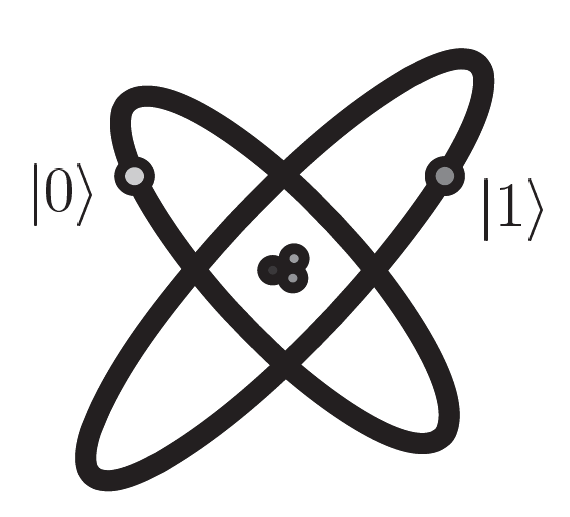
\includegraphics[scale=.4]{atom.png}
	\centering
	\caption{Qubit represented by two electron orbits in an atom, \cite{Nielsen2002}.}
	\label{fig 1.1}
\end{figure}


\section{Postulate 3: Evolution}


The third postulate of quantum mechanics modulates the evolution of a quantum system. That is, the evolution of the state vector that describes the system. In order to properly formalize it we need the concepts of eigenvector and eigenvalues, as well as the Hermitian operators.


\subsection{Eigenvalues and eigenvectors}


\begin{definition}
	Let $V$ be a vector space and $A$ an operator on $V$. An \emph{eigenvector} is a non zero vector $|v_\lambda\rangle$ such that $A|v_\lambda\rangle = \lambda|v_\lambda\rangle$ for a complex value $\lambda$ called the associated \emph{eigenvalue}.
\end{definition}

Eigenvalues and associated eigenvectors will usually be denoted with the same letter for simplicity: $\lambda$ and $|\lambda\rangle$. We assume the reader is familiar with eigenvectors and values basic notions. For instance, that they may be calculated using the \emph{characteristic equation}: $|I - \lambda A| = 0$.

\begin{definition}
	A \emph{diagonal representation} of an operator $A$ is a representation $\sum_i \lambda_i |\lambda_i\rangle\langle\lambda_i|$ where the $|\lambda_i\rangle$ form an orthonormal set of A's eigenvectors and $\lambda_i$ are the respective eigenvalues. An operator is said to be \emph{diagonalizable} if it allows a diagonal representation.
\end{definition}

\begin{exampleth}
	As an example of this, let us consider the following matrix:
	
	$$ Z = 
	\begin{pmatrix}
		1 & 0 \\
		0 & -1 
	\end{pmatrix}
	$$
	
	This matrix is called the \emph{Z Pauli} matrix. It is relevant for quantum computing and it will be introduced later on along with the rest of the Pauli matrices. For now, lets compute its diagonalizable representation. Since it is already diagonal we can infer that its eigenvalues are $\{1, -1\}$. Computing the diagonal representation we realize that a pair orthonormal eigenvectors are $\{|0\rangle, |1\rangle\}$ respectively. Therefore:
	
	$$ Z = 
	\begin{pmatrix}
		1 & 0 \\
		0 & -1 
	\end{pmatrix} = 
	|0\rangle\langle0| - |1\rangle\langle1|
	$$
\end{exampleth}

Normal operators have significant relevancy thanks to the following result:

\begin{theorem}[Spectral Decomposition Theorem]
	An operator $A$ is normal if and only if it is diagonalizable.
\end{theorem}
\begin{proof}
	TODO: To be copied, Box 2.2, page 72, Nielsenchen.
\end{proof}

Since Hermitian and unitary operators are normal, we obtain the following result:

\begin{corollary}
	Any Hermitian operator is diagonalizable. Any unitary operator is diagonalizable.
\end{corollary}


\subsection{Postulate 3 statement}


\begin{postulate}
	The evolution of a \emph{closed} quantum system is described by a\emph{unitary transformation}. That is, the state $|\varphi\rangle$ of the system at time $t_1$ is related to the state $|\varphi'\rangle$ of the system at time $t_2$ by a unitary operator $U$ which depends only on the times $t_1$ and $t_2$,
	
	$$ |\varphi'\rangle = U|\varphi\rangle $$
\end{postulate}

It is worth mentioning that this postulated assumes our physical system to be \emph{isolated}. That is, there is no interaction with the system coming from the exterior. In reality, the only real closed system is the universe as a whole. However, we can recreate sufficiently closed systems so that they can be described with approximations as being closed. 

Just like the first postulate does not provide the state space or state vector of the system, the second postulate does not provide the unitary transformation that concretes this evolution. For our quantum computing case, we will be the ones to define the unitary transformation applied to the system. That is, the quantum circuit that transforms our qubit.

The description of the system evolution provided by \ref{postulate 2} only provides information for those fixed times $t_1$ and $t_2$. A continuous time description of this evolution is provided by the Schrodinger equation, which provides a redefinition of the second postulate.

\begin{postulate}
	The time evolution of the state of a \emph{closed} quantum system is described by the Schrodinger equation:
	
	$$ i \hbar \frac{d|\varphi\rangle}{dt} = H|\varphi\rangle $$
	
	where $\hbar$ is \emph{Planck’s constant}, $i$ is the imaginary unit and $H$ is a fixed Hermitian operator known as the $Hamiltonian$.
\end{postulate}

There are several notes to make about this postulate. First, the Hamiltonian is fixed for the given system and it is not be confused with the \emph{Hadamard quantum gate}, also represented by an $H$. Second, $\hbar$ is a physical constant that can be absorbed into the Hamiltonian for our purposes, simplifying the equation. Finally, this is a differential equation, so by knowing the initial state space of the system and the exact Hamiltonian we may know the exact evolution of the system.

Lets study the Hamiltonian in general. Since it is a Hermitian operator, it allows a spectral decomposition by the spectral decomposition theorem (TODOref Spectral Decomposition theorem):

$$ H = \sum_E E |E\rangle\langle E| $$

where $E$ are the eigenvalues and $|E\rangle$ the respective eigenvectors. 


TODO: O bien aquí o bien en otro sitio, comentar el ejemplo de Manzano sobre medidas respecto de los estados energéticos


\subsection{Quantum Computing perspective: ?}

In practice, obtaining the Hamiltonian for a given quantum system is a really laborious work and usually needs experimental data (TODO: add evidence? stated as such in Niel.). However, for our computational purposes we will be the ones designing the Hamiltonian such that our system evolves as desired. In particular, chapter 3 (TODO: add ref to QUBO chapter) describes in detail the construction of Hamiltonians for QUBO problems.

TODO: Completar



\section{Postulate 4: Composite systems}

\subsection{Tensor product}

\subsection{Postulate 4 statement}


\subsection{Quantum Computing perspective: Multiple qubits}


Suppose we have a pair of qubits. In the classical case, two bits can be in four possible states: 00, 01, 10, and 11. Similarly, the two qubits computational basis states are $|00\rangle$, $|01\rangle$, $|10\rangle$ and $|11\rangle$. Just like in the single qubit case, our two qubits system may be in a superposition of these four states:

$$ |\varphi\rangle = \alpha_{00} |00\rangle + \alpha_{01} |01\rangle + \alpha_{10} |10\rangle + \alpha_{11} |11\rangle $$

Correspondingly, the measurement of this system will result in either 00, 01, 10 or 11. In fact, it will yield state $x$ with probability $|\alpha_x|^2$, being $\alpha_x$ the coefficient associated with the state $|x\rangle$. The condition of the probabilities adding up to one is called the \emph{normalization condition} and can be expressed as $\sum_{x \in \{0,1\}^2} |\alpha_x|^2 = 1$ for the two qubits case, where $\{0,1\}^2$ are the strings of length two where each character is either $0$ or $1$.

The fundamental differences with the single qubit case start on measurement. Of course, we can measure both qubits at the same time, but we could also measure only one of them. Upon measuring the first qubit we would obtain $0$ with probability $p_0 = |\alpha_{00}|^2 + |\alpha_{01}|^2$, since these are the coefficients associated with the first qubit being $0$. Furthermore, our system will collapse to:

$$ |\varphi'\rangle = \frac{ \alpha_{00} |00\rangle +f \alpha_{01} |01\rangle }{ \sqrt{|\alpha_{00}|^2 + |\alpha_{01}|^2} } $$

Note the normalization term $\sqrt{|\alpha_{00}|^2 + |\alpha_{01}|^2}$, applied so the post-measurement state still satisfies the normalization condition. Naturally, after obtaining $0$ in the first qubit we can still obtain either $0$ or $1$ in the second qubit, with probabilities 

$$ \frac{ |\alpha_{00}|^2 }{ |\alpha_{00}|^2 + |\alpha_{01}|^2 }  \ \text{ and } \ 
\frac{ |\alpha_{01}|^2 }{ |\alpha_{00}|^2 + |\alpha_{01}|^2 } $$

respectively, adding up to $1$. Correspondingly, the first qubit being measured will yield $1$ with probability $p_1 = |\alpha_{10}|^2 + |\alpha_{11}|^2$.

Additionally, the first qubit independently should satisfy the normalization condition. That is, its probabilities of being $0$ and $1$ upon measurement must add up to $1$. But those are $p_0$ and $p_1$, which add up to one because of the normalization condition for $|\varphi\rangle$, as expected.

We now introduce the \emph{Bell State} or \emph{EPR pair:}

$$ \frac{ |00\rangle + |11\rangle }{ \sqrt 2 } $$

Although it may seem harmless at first glance, this state has been responsible for many surprises during the development of quantum physics [TODOref to the EPR paradox]. Let us have a first look into it, although we will come back to it in section [TODOref la seccion dodne comentamos el problema de la teletransportación cuántica].

Upon measuring this system we may obtain state $|00\rangle$ with probability $1/2$ and state $|11\rangle$ with probability $1/2$. Suppose we measure the first qubit and obtain $0$. Then, the second qubit will always yield $0$ upon measurement. This means both outcomes are \emph{correlated}. This fact is known as \textbf{quantum entanglement}. It rests at the heart of the disparity between classic physics and quantum physics. It was deeply studied first by Einstein, Podolsky, and Rosen (EPR) \cite{Einstein1935} and second by John Bell \cite{Bellt1964}.

Let us finally consider the more general case. In an n-qubits system our computational basis would consist of the sates $|x_1 x_2 \dotsc x_n\rangle$, where $x_i \in \{0,1\}$. As we already know, in a single qubit system we have two amplitudes $\alpha_0$ and $\alpha_1$. We have four amplitudes for a 2-qubits system, eight for a 3-qubits system... And $2^n$ for an n-qubits system. This means that the number of amplitudes grows exponentially as we add qubits to the system. An immense increment concerning the classical case was the quantity of information that our simple holds grows linearly with the numbers of bits. Of course, we already know it is not that simple, since there are huge limitations on how we may access this information in the quantum realm such as how a qubit collapses upon measurement and the non-cloning theorem discussed in section [TODO]. But we can already glimpse the power of quantum computing versus the classical one.


\chapter{The D-Wave Quantum Computer}


In this second chapter, we aim to understand the D-Wave Quantum systems. In order to achieve that, we start by explaining the basis of quantum annealing that the D-Wave systems used underneath, and how to transform problems into the adequate format for these systems.


\section{Quantum Annealing}


Simulated annealing (SA) is a general optimization technique that was first introduced in 1983 by Kirkpatrick \emph{et al.} \cite{Kirkpatrick1983}. The main idea is to mimic how thermal fluctuations works to let the system escape from local minimums in the cost function. The \emph{temperature} of the system dictates the probability with which the is allowed to jump to worse solutions (higher values of the cost function). The \emph{annealing schedule} is the decrease rate of the temperature, controlled by the programmer. Under the appropriate one, the system would be able to escape from local minimums to reach the global one. If the temperature decreases too quickly, the system converges prematurely to a local minimum. If it decreases too slowly, the technique transforms into a random walker, reaching the global minimum at some point but being worthless time-wise.

Inspiration in thermal fluctuations is used in SA so the system may escape from local minima. Similarly, \emph{quantum tunneling} is used in Quantum Annealing (QA) to escape from local minimums. This new technique was introduced in its present form by two similar proposals \cite{Finnila1994} \cite{Kadowaki1998}.

Quantum tunneling is a quantum mechanical phenomenon where a wavefunction (i.e. a quantum state) may propagate through a potential barrier \cite{Nimtz2008}. The probability of this event occurring depends on the height and width of the barrier (see figure \ref{fig 2.1})

\begin{figure}[h]
	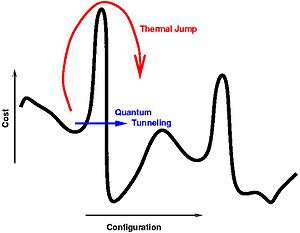
\includegraphics[scale=.8]{QuantumTunneling.jpg}
	\centering
	\caption{Thermal jumps vs quantum tunneling.}
	\label{fig 2.1}
\end{figure}

The main advantage of quantum tunneling compared to classical thermal fluctuations is that the probability of the system shifting depends not only on the height of the potential barrier but also on its width. Thus, the application of QA may potentially outperform SA in problems where the energy (cost) landscape consists of very high and thin barriers surrounding local minimums. 

Particularly, as studied in \cite{Ray1989}, let $\Delta$ be the height of a barrier and $\omega$ its width. The probability of a thermal transition occurring is dictated by $exp\{-\frac{\Delta}{k_B T}\}$ where $T$ y the temperature of the system and $k_B$ is the Boltzmann constant. On the other hand, the probability of a quantum tunneling transition occurring through the same barrier (assuming isolation) is $exp\{-\frac{\sqrt \Delta \omega}{\Gamma}\}$, where $\Gamma$ is the tunneling field. Thus, the probability is much higher for the quantum tunneling effect on high and thin barriers.

We may also observe looking at the previous expressions how the tunneling field and the temperature play similar roles in the different methods. Thus, the annealing schedule of the QA system is controlled using the tunneling field just like the temperature is used in SA.

There are many examples in the literature of QA simulations using classical computers, both theoretical \cite{Morita2008} and numerical -most of them using Quantum Monte Carlo (QMC) methods \cite{Isakov2016} \cite{Farhi2000}-. This evidence suggests the outperformance of SA by simulated QA under certain conditions. It is reasonable to wonder what happens if instead of simulating QA we could somehow encode our problems in a real physical system that tends to its lower energy state (ground state), thus using quantum tunneling naturally. This is precisely what the D-Wave system does.

Let us further deepen into the technicalities of quantum annealing in order to understand how it is implemented in the D-Wave system.


\section{Adiabatic Evolution}
\label{sec:adiabatic-evolution}


The alternative form of the third postulate of quantum mechanics (section \ref{sec:postulate-3}) stated that the evolution of a quantum system is described by the Schrodinger equation:

$$ i \hbar \frac{d|\varphi\ra}{dt} = H|\varphi\ra $$

By better understanding the Hamiltonian $H$ we may control this evolution. Suppose that the evolution of a given quantum system is described by a Hamiltonian $\hat H(t)$. Suppose that at some initial time $t_0$ our quantum system is in an eigenstate $|\varphi(t_0)\ra$ of $\hat H(t_0)$. Since the evolution is continuous, at some other time $t_1 > t_0$ we could expect our system to be in the corresponding eigenstate $|\varphi(t_1)\ra$ of $\hat H(t_1)$. This fact critically depends on the time $\tau = t_1 - t_0$ during which the modification takes place, as stated by the adiabatic theorem, first proposed by Max Born and Vladimir Fock (1928) \cite{Born1928}.

\begin{theorem}[Adiabatic Theorem]
	\label{th:adiabatic-theorem}
	A physical system remains in its instantaneous eigenstate if a given perturbation is acting on it slowly enough and if there is a gap between the eigenvalue and the rest of the Hamiltonian's spectrum.
\end{theorem}

Thus, we may define diabatic and adiabatic processes depending on how they adapt to the system changes \cite{Kato1950}.

\begin{definition}
	A \emph{diabatic process} is a process where rapidly changing conditions prevent the system from adapting its configuration during the process. Typically there is no eigenstate of the final Hamiltonian with the same functional form as the initial state. The system ends in a linear combination of the states.
\end{definition}

\begin{definition}
	An \emph{adiabatic process} is a process where gradually changing conditions allow the system to adapt its configuration. If the system starts in an eigenstate of the initial Hamiltonian, it will end in the corresponding eigenstate of the final Hamiltonian.
\end{definition}

The 'gap condition' that appears in theorem \ref{th:adiabatic-theorem} refers to an additional requirement: the spectrum of $\hat H(t)$ is \emph{nondegenerate}, meaning there are no two equal eigenvalues at fixed time $t$. This condition is also called the \emph{no-crossing} condition and allows us to sort the eigenstates using the eigenvalues without any ambiguity.

As a classical analogy for adiabatic evolution, consider a simple pendulum. If the pendulum's support point is moved, the oscillation of the pendulum may change. In fact, violent changes on the support point will dramatically affect the pendulum's movement, changing it completely. However, if the support point is moved slowly enough, the pendulum will remain unchanged. These are examples of diabatic and adiabatic processes respectively.


\subsection{Avoided crossing}


Let us consider an important physical example known as the \emph{avoided crossing}. Consider a two-state quantum system, i.e. a qubit. Suppose its Hamiltonian to be:

$$
	H = 
	\begin{pmatrix}
		E_1 & 0 \\
		0 & E_2 
	\end{pmatrix}
$$

Whose eigenvalues are $E_1$ and $E_2$, and eigenvectors,

$$
	|0\ra = 
	\begin{pmatrix}
	1 \\
	0 
	\end{pmatrix}, \quad
	|1\ra = 
	\begin{pmatrix}
	0 \\
	1 
	\end{pmatrix}
$$

which will be used as our base. Thus, a state vector describing the system may be written as a superposition of both states:

$$ |\varphi\ra = \alpha|0\ra + \beta|1\ra $$

Supposing adiabatic evolution, if the system is prepared in either one of the eigenstates it will remain as such as long as the gap condition is sufficed: $E_1 \neq E_2$. However, if $E_1 = E_2$, any superposition of states will be an eigenstate, thus remaining unchanged. Hence, independently of $E_1$ and $E_2$, any system prepared in an eigenstate will remain as such, supposed adiabatic evolution.

Let us consider a perturbation $P$ into our original system. For simplicity, we only consider perturbations with degenerated diagonal. Our new Hamiltonian will be the following:

$$
	H' = H + P =
	\begin{pmatrix}
	E_1 & 0 \\
	0 & E_2 
	\end{pmatrix} +
	\begin{pmatrix}
	0 & \omega \\
	\overline \omega & 0 
	\end{pmatrix} = 
	\begin{pmatrix}
	E_1 & \omega \\
	\overline \omega & E_2 
	\end{pmatrix}
$$

where $\omega \in \C$. Note that by setting $\omega$, the other value in the antidiagonal is fixed since $H'$ must be Hermitian. By using the characteristic equation we may compute the eigenvalues of $H'$:

$$ E_+ = \frac{1}{2}(E_1 + E_2) + \frac{1}{2}\sqrt{(E_1 - E_2)^2 + 4|\omega|^2} $$
$$ E_- = \frac{1}{2}(E_1 + E_2) - \frac{1}{2}\sqrt{(E_1 - E_2)^2 + 4|\omega|^2} $$


A continuación quiero añadir una imagen, seguramente como la de \href{https://en.wikipedia.org/wiki/Avoided_crossing}{wikipedia} (figura \ref{temp}):

\begin{figure}[H]
	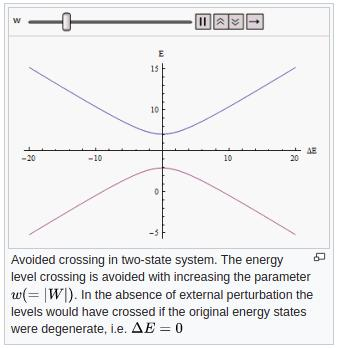
\includegraphics[scale=1]{wiki.jpg}
	\centering
	\caption{Figura de wikipedia}
	\label{temp}
\end{figure}

He hecho una versión propia en Geogebra, tomando $E_1 = -E_2$ (luego $E_1 + E_2 = 0$ y $E_1 - E_2 = 2E$, he llamado $x \equiv 2E$). En la simulación, podemos ajustar el valor de $\omega$, que he llamado $a$ utilizando el slider, reproduciendo el efecto del gif de \href{https://en.wikipedia.org/wiki/Avoided_crossing}{wikipedia} (figura \ref{temp}):

\href{https://www.geogebra.org/graphing/svkrnu3s}{https://www.geogebra.org/graphing/svkrnu3s}

Sin embargo, me salen las ramas de las hiperbolas giradas 90 grados. Esperaba que la rama superior fuese $E_+$ y la inferior $E_-$ pero cada rama tiene parte de las dos. Cual es mi fallo al pintar las gráficas?

%TODO2: Explicar que pasa cuando variamos ($E_1 - E_2$) y pintarlo en geogebra bonito
%TODO3: Conclusion: en un qubit siempre se da el gap.
%TODO4: Explicar que pasa en evolucion no adiabatica.
%TODO5: relacion con quantum annealing


%TODO: añadir autoria a las imagenes



\subsection{Solving problems using adiabatic evolution}


In order to use adiabatic evolution to solve optimization problems we will configure our own Hamiltonian for the system. In particular, the Hamiltonian will be a time-dependent linear combination of two constant Hamiltonians:

$$ H(t) = f(t) \cdot H_{initial} + g(t) \cdot H_{final} \quad \forall t \in [t_{initial}, t_{final}] $$

where $f,g: [t_{initial}, t_{final}] \longrightarrow \R^+_0$. The initial Hamiltonian, $H_{initial}$, will be an easy configuration so we may prepare our system to start in the ground state of $H_{initial}$. The final Hamiltonian, $H_{final}$, will encapsulate the cost function of our problem such that the minimum value is reached in the ground state. 

Functions $f$ and $g$ fulfill that $g(t_{initial}) = f(t_{final}) = 0$. When times elapses and supposing adiabatic evolution, the system will stay on the ground state of $H$ and by $t = t_{final}$, the system will be in the $H_{final}$'s ground state, codifying the minimum of our cost function.

However, we cannot always grant the necessary conditions for perfect adiabatic evolution. In some cases, the gap condition does not suffice at the system will jump with a certain probability to other eigenstates, providing suboptimal solutions which are still useful. This depends on the eigenvalues of the final Hamiltonian, which at the same time entirely depends on the problem being studied.

The only question remaining is how to encode our cost function in a Hamiltonian.


\section{QUBO and Ising models}


The QUBO and Ising models can be easily represented with a Hamiltonian. In practice, non-optimization problems are transformed into optimization problems and then codified as either QUBO or Ising to be solved using quantum annealing. Let us explore these types of problems and some examples of these transformations.

Let $B = \{0,1\}$ and $f: \B^n \longrightarrow \R $ be a quadratic polynomial over binary variables:

$$ f_Q(x) = \sum_{i=1}^n \sum_{j=1}^i q_{ij} x_i x_j $$

where $x_i \in \B$ for $i \in \{1, \cdots, n\}$ and the coefficients $q_{ij} \in \R$ for $1 \leq j \leq i \leq n$. A \textbf{quadratic unconstrained binary optimization (QUBO) problem} consists of finding a binary vector $x'$ such that $x'$ is a minimum of $f$:

$$ x' = \underset {x \in \B^n }{\arg \min} ~ f(x) $$

QUBO problems can be formulated in a more compact matrix form:

$$ f_Q(x) = x^T Q x $$

where $Q$ is a $n \times n$ symmetric matrix containing $q_{ii}$ and its diagonal and $q_{ij} / 2$ in position $(i,j)$ where $i \neq j$. Let us explore some simple properties of QUBO problems:

\begin{itemize}
	\item Multiplying the coefficients $q_{ij}$ by a constant $a \in \R^+$ scales the output by exactly $a$. Thus, $x'$ remains the minimum:
	
		$$ f_{aQ}(x) = \sum_{i<j} (a q_{ij}) x_i x_j  = a \sum_{i<j} q_{ij} x_i x_j = a f_Q(x) $$
		
	\item Flipping the sign of the coefficients flips the sign of $f_Q(x)$. Thus, $x'$ is the maximum of $f_{-Q}(x)$
	
		$$ f_{-Q}(x) = \sum_{i<j} (-q_{ij}) x_i x_j  = - \sum_{i<j} q_{ij} x_i x_j = -f_Q(x) $$
		
	\item If all coefficients are positive the minimum is $x = (0, \ldots, 0)$. Analogously, if all coefficients are negative, the minimum is $x = (1, \ldots, 1)$. 
\end{itemize}

The \textbf{Ising models}, on the other hand, find their inspiration in phisics. They are named after the phisic Ernst Ising who solved the one-dimensional model in his 1924 thesis \cite{Ising1924}. They are stated using a Hamiltonian function $H: \{-1, 1\}^n \longrightarrow \R$:

$$ H(\upsigma) = - \sum_{\la i ~ j \ra} J_{ij} \upsigma_i \upsigma_j - \mu \sum_j h_j \upsigma_j $$

with parameters $h_j, J_{ij}, \mu \in \R$. The \emph{spin variables} $\upsigma_i$ are in $\{-1, 1\}$ instead of $\B$. Moreover, the spin variables are arranged in a graph, typically a \emph{lattice}, where a local structure repeats periodically. The only pair of variables $\la i ~ j \ra$ which are neighbor nodes in the graph may have non-zero coefficients $J_{ij}$. Let us see the connection between the QUBO and Ising models by using the identity $\upsigma \mapsto 2x -1$:

\begin{equation*}
	\begin{split}
		f(x)	& = \sum_{\la i ~ j \ra} - J_{ij} (2x_i - 1) (2x_j - 1) - \sum_j \mu h_j (2x_j - 1) \\
				& = \sum_{\la i ~ j \ra} - 4J_{ij} x_i x_j + 2J_{ij} x_i + 2J_{ij} x_j - J_{ij} + \sum_j 2 \mu h_j x_j - \mu h_j \qquad \text{using }  x_j = x_jx_j \\
				& = \sum_{i=1}^n \sum_{j=1}^i q_{ij} x_i x_j + C
	\end{split}
\end{equation*}

where 

\begin{equation*}
	q_{ij} = 
		\begin{dcases}
			-4 J_{ij} 																	& \text{if } i \neq j \\
			\sum_{\la k ~ i \ra} 2 J_{ki} + \sum_{\la i ~ l \ra} 2 J_{il} + 2 \mu h_i	& \text{if } i = j
		\end{dcases}
\end{equation*}

$$ C = - \sum_{\la i ~ j \ra} J_{ij} - \mu \sum h_j $$

Since adding a constant does not change the minimum $x'$, it can be omitted during optimization and only be used for transforming one type of problem into another.

In practice, a given problem would be translated into either QUBO or Ising. It is useful to learn both types of problems since they both are popular in the literature. Let us deepen in the translation of different NP problems. The resolution of QUBO and Ising models will not be studied, but only the translations into these models. In particular, these examples of QUBO transformations are from \cite{Glover2019} and \cite{Lucas2014} unless stated otherwise. For an extensive literature review on QUBO and Ising translations of NP, problems refer to \cite{Kochenberger2014}.


\subsection{The Max Cut problem}


One of the first famous problems that was encoded as a QUBO was the max-cut problem due to its natural translation. It reads as follows: Given an undirected graph $G(V, E)$ with vertex set $V$ and edge set $E$, seek a partition of $V$ such that the number of edges between both sets is as large as possible.

The max-cut problem can be modeled by setting variable $x_j = 1$ if vertex $j$ is in one set and $x_j = 0$ if it is in the other one, for every vertex $j$ in $V$. The quantity $(x_i + x_j - 2 x_i x_j)$ marks whether the edge $(i,j)$ is in the cut. That is, $(x_i + x_j - 2 x_i x_j) = 1$ if the vertices $x_i$ and $x_j$ are in different sets, and $0$ otherwise.

Thus, maximazing the number of edges in the cut is encoded as a QUBO as:

$$ \text{Maximize } f(x) = \sum_{(i,j) \in E} \big( x_i + x_j - 2 x_i x_j \big) $$


\newparagraph{Numerical example}


Consider the following graph:

\begin{figure}[H]
	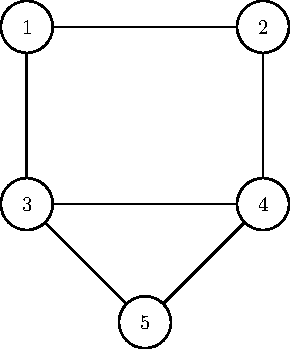
\includegraphics[scale=1]{graphs/max-cut-example.pdf}
	\centering
\end{figure}

We would have five variables: $x_1, \cdots, x_5$. The cost associated to edge $(1,2)$ is $x_1 + x_2 - 2 x_1 x_2$. By repeating this process for every edge in the graph we obtain the cost function:

$$ \text{Maximize  } f(x) = (x_1 + x_2 - 2 x_1 x_2) + (x_1 + x_3 - 2 x_1 x_3) + (x_2 + x_4 - 2 x_2 x_4) $$
$$ +(x_3 + x_4 - 2 x_3 x_4) + (x_3 + x_5 - 2 x_3 x_5) + (x_4 + x_5 - 2 x_4 x_5) $$

or equivalently:

$$ \text{Maximize  } f(x) = 2x_1 + 2x_2 + 3x_3 + 3x_4 + 2x_5$$ 
$$ - 2x_1x_2 - 2x_1x_3 - 2x_2x_4 - 2x_3x_4 - 2x_3x_5 - 2x_4x_5 $$

We can transform the problem using the following symmetric matrix:

$$
	Q = 
	\begin{pmatrix}
	2 & -1 & -1 & 0 & 0 \\
	-1 & 2 & 0 & -1 & 0 \\
	-1 & 0 & 3 & -1 & -1 \\
	0 & -1 & -1 & 3 & -1 \\
	0 & 0 & -1 & -1 & 2
	\end{pmatrix}
$$

Yielding the following compact form:

$$ \text{Maximize  } f_Q(x) = x^T Q x$$ 

By solving this model using quantum annealing we obtait the minimum value of $f_Q(x)$: $x = (0, 1, 1, 0, 0)$. Thus, vertices $2$ and $3$ are in one set and vertices $1$, $4$ and $5$ are in the other one.


\subsection{General translation method}

The previous problem was naturally transformed into QUBO due to its particular constraints. However, can any quadratic optimization problem be encoded as a QUBO?

The answer to this question is positive. Furthermore, any quadratic optimization problem with linear constraints may be transformed into a QUBO. Let us first study a simple case. Consider the following problem:

\begin{gather*}
	\text{Minimize } f(x_1, x_2) \\
	\text{subject to the constraint} \\
	x_1 + x_2 \leq 1
\end{gather*}

where $x_1, x_2 \in \B$. We may transform our linear constraint into a penalty $P(x_1x_2)$ for some positive scalar $P$. This term equals $0$ if and only if our constraint is satisfied by the variables. Thus, by adding the penalty to our cost function, for $P$ large enough, the problem

\begin{gather*}
	\text{Minimize } f(x_1, x_2) + Px_1x_2
\end{gather*}

will minimize $f(x_1, x_2)$ and, at the same time, satisfy the constraint. Namely, the constraint translates into adding a non-negative value to the cost function. Some other useful translations can be found in table \ref{tab:penalties-table}. In general, if the cost function is being minimized we may substitute constraints by non-negative terms that only equal zero if they are satisfied, multiplied by a large enough positive value $P$. Thus, we may remove the associated constraints by simply adding these terms to the cost function.

\begin{table}[h]
	\centering
	\begin{tabular}{cc}
		Classical Constraint 		& Equivalent Penalty   			\\ \hline
		$x + y \leq 1$       		& $P(xy)$              			\\
		$x + y \geq 1$       		& $P(1 - x - y + xy)$  			\\
		$x + y = 1$          		& $P(1 - x - y + 2xy)$ 			\\
		$x \leq y$       			& $P(x - xy)$      
		
		   			\\
		$x_1 + x_2 + x_3 \leq 1$	& $P(x_1x_2 + x_1x_3 + x_2x_3)$	\\
		$x = y$              		& $P(x + y - 2xy)$    
	\end{tabular}
	\caption{Constraints and penalties relations}
	\label{tab:penalties-table}
\end{table}

Specifically, let us study the more general case:

$$ \text{Minimize } f(x) = x^T C x $$
$$ \text{subject to the constraints} $$
$$ Ax = b $$

where $x \in \B^n$, $k$ is the number of constraints, $b \in \R^k$, $C$ is a $n \times n$ real matrix and $A$ is a $k \times n$ real matrix. This accomodates to both linear and quadratic cost function since elements in the diagonal are $c_{ii} x_i^2 = c_{ii} x_i$. For a positive scalar $P$, the quadratic penalty $P (Ax - b)^T (Ax - b)$ is added to the cost function to obtain:

\begin{equation*}
	\begin{split}
		f'(x)	& = x^T C x + P (Ax - b)^T (Ax - b) \\
		& = x^T C x + P (x^TA^TAx - \cancelto{}{x^TA^Tb} - \cancelto{}{b^TAx} + b^Tb) \\
		& = x^T C x + x^T D x + c \\
		& = x^T Q x + c 
	\end{split}
\end{equation*}

where $D = P(A^TA)$, $c = P(b^Tb)$ and $Q = C + D$. Since the constant $c$ does not affect where the minimum is reached, $f$ and $f'$ share this minimum. Therefore, we may simply solve:

$$ \text{Minimize } f(x) = x^T Q x $$

which is a QUBO problem.

In this development, we only considered equality constraints. There is also a general method to transform inequality constraints into equality ones by introducing \emph{slack variables} \cite{Hull2003}. In practice, the general case will not be necessary since the constraints are usually quite simple.

Finally, we may also consider satisfiability problems. That is, given a set of constraints for the variables, find a configuration of them such that all the constraints are satisfied. If the constraints are linear, these problems may be transformed into QUBO by setting the cost function as constant and following the same method. Suppose the constraints over $x$ can be written as $Ax = b$. The equivalent optimization problem is written as:

$$ \text{Minimize } f(x) = 0 $$
$$ \text{subject to the constraints} $$
$$ Ax = b $$

Any solution satisfying the constraint will yield $0$ on the penalties, thus minimizing the transformed cost function $f'(x) = x^T Q x$. 

Let us explore some more complicated examples to expand on these ideas.


\subsection{Satisfiability problems: Max 2-SAT}


This example is based on \cite{Glover2019} and \cite{Farhi2000}.

In the previous section, we mentioned satisfiability problems, also known simply as SAT. In this section, we study these problems from its traditional logic perspective.

A \emph{clause} is statement depending on a finite set of binary variables , $C = C(x_1, \ldots, x_k)$, that be either True or False. A \emph{literal} is a variable or its negation: $x$ and $\neg x$ are literals. Let $C_1, \ldots, C_n$ be a set of \emph{Clauses} depending on variables $x_1, \ldots, x_m$. The satisbiality problem associated to this problem is to find a configuration for the variables $x_1, \ldots, x_m$ such that every clause is true:

$$ C_1 \wedge \cdots \wedge C_n $$

SAT was the first problem proven to be NP-complete. This result is known as the Cook-Levin theorem, named after Stephen Cook and Leonid Levin \cite{Book1980}. Its relevance in computer science is astronomical. There have been many variations of SAT problems, let us explore one of them, the Max 2-SAT variation, and transform it into a QUBO model.

Max 2-SAT problem is an optimization problem. Its main restriction is that each clause may depend on at most two literals and it is true if and only if at least one literal is true. The problem consists of finding a configuration of variables such that the number of true clauses is maximized. Each clause $C(x_C, y_C)$ is associated with an energy function depending on the variables $(x_C, y_C)$:

\begin{equation*}
E_C(x_C, y_C) = 
\begin{dcases}
0,	& \text{if } (x_C, y_C) \text{ satisfies clause } C \\
1,	& \text{if } (x_C, y_C) \text{ violates clause } C \\
\end{dcases}
\end{equation*}

The energy of the whole system, which will work as our cost function, is defined as the sum of all the energies:

$$E = \sum_C E_C$$

Clearly $E \geq 0$ and $E = 0$ if and only if every clause is true. Furthermore, the minimum energy of the system $E_0$ will be reached where the maximum number of clauses are satisfied: exactly every clause but $E_0$ will be true. Note that this perspective does not depend on the Max 2-SAT problem. In fact, the same process is used to transform other satisfiability problems.

The remaining question is how to transform our clauses into energy functions. For the Max 2-SAT problem this is quite straightforward. Each clause may depend on at most two literals. Thus, there are either zero, one, or two negations in each clause. We may study this cases separately, as seen in table \ref{tab:penalties-max-2-sat-table}.

\begin{table}[h]
	\centering
	\begin{tabular}{ccc}
		Clause 					& Traditional constraing	& Energy function		\\ \hline
		$x \vee y$       		& $x + y \geq 1$    		& $(1 - x - y + xy)$	\\
		$\neg x \vee y$      	& $\neg x + y \geq 1$ 		& $(x - xy) $  			\\		
		$\neg x \vee \neg y$    & $\neg x + \neg y \geq 1$ 	& $(xy)$ 
	\end{tabular}
	\caption{Clause and energy functions relations}
	\label{tab:penalties-max-2-sat-table}
\end{table}

Since every energy function is quadratic, the total energy will also be quadratic. This is the cost function used in our QUBO model:

$$ \text{Minimize } E(x) = \sum_C E_C$$

Note that, interestingly enough, our QUBO model does not depend on the number of clauses but only on the number of variables. This means that a problem with $30.000$ clauses and $200$ variables will only use $200$ variables in the associated QUBO model.


\newparagraph{Numerical Example}


Given the following set of clauses found in table \ref{tab:penalties-max-2-sat-example}, find a solution to the Max 2-SAT problem associated with them.

\begin{table}[h]
	\centering
	\begin{tabular}{ccc}
		Clause $\#$	& Clause						& Energy function				\\  		\hline
		1       	& $x_1 \vee x_2$    			& $(1 - x_1 - x_2 + x_1x_2)$	\\
		2       	& $x_1 \vee \neg x_2$    		& $(x_2 - x_1x_2)$				\\
		3       	& $\neg x_1 \vee x_2$    		& $(x_1 - x_1x_2)$				\\
		4       	& $\neg x_1 \vee \neg x_2$    	& $(x_1x_2)$					\\
		5       	& $\neg x_1 \vee x_3$    		& $(x_1 - x_1x_3)$				\\
		6		  	& $\neg x_1 \vee \neg x_3$    	& $(x_1x_3)$					\\
		7       	& $x_2 \vee \neg x_3$    		& $(x_3 - x_2x_3)$				\\
		8       	& $\neg x_2 \vee x_3$    		& $(x_2 - x_2x_3)$				\\
		9       	& $\neg x_2 \vee \neg x_3$    	& $(x_2x_3)$					\\
		10       	& $x_2 \vee x_4$    			& $(1 - x_2 - x_4 + x_2x_4)$	\\
		11       	& $x_3 \vee x_4$    			& $(1 - x_3 - x_4 + x_3x_4)$	\\
		12       	& $\neg x_3 \vee \neg x_4$    	& $(x_3x_4)$					
	\end{tabular}
	\caption{Clause and energy functions relations}
	\label{tab:penalties-max-2-sat-example}
\end{table}

A quick look at the first four clauses tells us that we cannot possibly find a configuration of variables that satisfy every clause. In fact, at most three of those four will be true. Adding the energies associated with every clause gives us the energy of the system, and therefore our QUBO model:

$$ \text{Minimize } E(x) = 3 + x_1 - 2 x_4 - x_2x_3 + x_2x_4 + 2 x_3x_4 $$

or equivalently:

$$ \text{Minimize } E(x) = 3 + x^T Q x $$

where

$$
Q = 
\left(
\begin{array}{cccc}
	1 & 0 & 0 & 0 \\
	0 & 0 & -1/2 & 1/2 \\
	0 & -1/2 & 0 & 1 \\
	0 & 1/2 & 1 & -2 
\end{array}
\right)
$$

Solving this QUBO gives $x_1 = x_2 = x_3 = 0$ and $x_4 = 1$ with energy $E(0, 0, 0, 1) = 1$, meaning that all clauses but one are satisfied.

As a final remark, this method of solving Max 2-SAT problems has proven to be computationally useful up to hundreds of variables and thousands of clauses \cite{Kochenberger2005}.


\subsection{Graph Coloring}


Consider the following problem: Given a graph $G$ and $K$-colors, assign a single color to each vertex in $V$ such that no two adjacent vertices have the same color. Let $x_{ij}$ be a binary variable that is set to $1$ if and only if the $i$-th node is assigned the color $j$-th. We may develop the following two constraints. First, since all nodes must be colored exactly once:

$$ \sum_{j=1}^K x_{ij} = 1 \quad \forall i \in \{1, \cdots, n\} $$

where $n$ is the number of nodes. Moreover, the condition that two adjacent nodes cannot have the same color is translated into:

$$ x_{ic} + x_{jc} \leq 1 \quad \forall c \in \{1, \cdots, K\} $$

for every pair of adjancent nodes $(i,j)$ in $G$.

Thus, by finding a vector configuration for the variables $x_{ij}$ that satisfy this constraint, we find a solution to the graph coloring problem. This is what we previously introduced as a satisfiability problem. Therefore, it may be written as:

$$ \text{Minimize } f(x) = 0 $$
$$ \text{subject to the constraints} $$
$$ \sum_{j=1}^K x_{ij} = 1 \quad \forall i \in \{1, \cdots, n\} \quad \text{and}$$
$$ x_{ic} + x_{jc} \leq 1 \quad \forall c \in \{1, \cdots, K\} \quad \text{for all adjacent nodes i and j}$$


\newparagraph{Numerical Example}


Given the following graph, find a coloring using three colors.

\begin{figure}[H]
	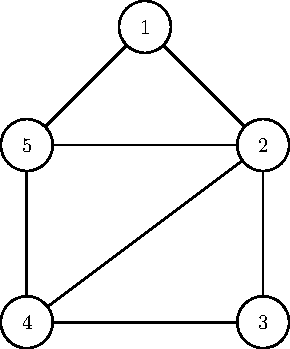
\includegraphics[scale=1]{graphs/graph-coloring-example.pdf}
	\centering
\end{figure}

For this particular graph there are $15$ variables: $x_{ij}$ for all $i \in \{1, \cdots, 5\}$ and for all $j \in \{1, 2, 3\}$. The associated constraints are:

$$ x_{i1} + x_{i2} + x_{i3} = 1 \quad \forall i \in \{1, \cdots, 5\} $$
$$ x_{ic} + x_{jc} \leq 1 \quad \forall c \in \{1, 2, 3\} \quad \text{for all adjacent nodes i and j} $$

a total of $26$: $5$ for assigning one and only one color to each node, and $3$ additional ones per edge in the graph ($7$) for no adjacent equally colored nodes. First, let us rename our variables from $1$ to $15$ as follows:

$$ (x_{11}, x_{12}, x_{13}, x_{21}, x_{22}, x_{23}, x_{31}, \dots, x_{52}, x_{53}) =
	(x_1, x_2, x_3, x_4, x_5, x_6, x_7, \dots, x_{15}, x_{16}) $$

The first set of constraints may be substitued by $P(x_{i1} + x_{i2} + x_{i3} - 1)^2$, which only equals $0$ if the constraint is satisfied. For instance, for the first node $P(x_1 + x_2 + x_3 - 1)^2$ is tranformed to $P(- x_1 - x_2 - x_3 + 2 x_1 x_2 + 2 x_1 x_3 + 2 x_2 x_3 + 1)$. By chosing a value for $P=4$ and dropping the constant we can  insert these penalties into an under developed $Q$ matrix:

$$
Q = 
\left(
\begin{array}{*{15}c}
	-4 & 4 & 4 & 0 & 0 & 0 & 0 & 0 & 0 & 0 & 0 & 0 & 0 & 0 & 0 \\
	4 & -4 & 4 & 0 & 0 & 0 & 0 & 0 & 0 & 0 & 0 & 0 & 0 & 0 & 0 \\
	4 & 4 & -4 & 0 & 0 & 0 & 0 & 0 & 0 & 0 & 0 & 0 & 0 & 0 & 0 \\
	0 & 0 & 0 & -4 & 4 & 4 & 0 & 0 & 0 & 0 & 0 & 0 & 0 & 0 & 0 \\
	0 & 0 & 0 & 4 & -4 & 4 & 0 & 0 & 0 & 0 & 0 & 0 & 0 & 0 & 0 \\
	0 & 0 & 0 & 4 & 4 & -4 & 0 & 0 & 0 & 0 & 0 & 0 & 0 & 0 & 0 \\
	0 & 0 & 0 & 0 & 0 & 0 & -4 & 4 & 4 & 0 & 0 & 0 & 0 & 0 & 0 \\
	0 & 0 & 0 & 0 & 0 & 0 & 4 & -4 & 4 & 0 & 0 & 0 & 0 & 0 & 0 \\
	0 & 0 & 0 & 0 & 0 & 0 & 4 & 4 & -4 & 0 & 0 & 0 & 0 & 0 & 0 \\
	0 & 0 & 0 & 0 & 0 & 0 & 0 & 0 & 0 & -4 & 4 & 4 & 0 & 0 & 0 \\
	0 & 0 & 0 & 0 & 0 & 0 & 0 & 0 & 0 & 4 & -4 & 4 & 0 & 0 & 0 \\
	0 & 0 & 0 & 0 & 0 & 0 & 0 & 0 & 0 & 4 & 4 & -4 & 0 & 0 & 0 \\
	0 & 0 & 0 & 0 & 0 & 0 & 0 & 0 & 0 & 0 & 0 & 0 & -4 & 4 & 4 \\
	0 & 0 & 0 & 0 & 0 & 0 & 0 & 0 & 0 & 0 & 0 & 0 & 4 & -4 & 4 \\
	0 & 0 & 0 & 0 & 0 & 0 & 0 & 0 & 0 & 0 & 0 & 0 & 4 & 4 & -4 
\end{array}
\right)
$$

Secondly, in order to transform $x + y \leq 1$ we can refer to table \ref{tab:penalties-table} and use $P(xy)$. We add these penalties to the previous matrix in the proper places:

$$
Q = 
\left(
\begin{array}{*{15}c}
	-4 & 4 & 4 & 2 & 0 & 0 & 0 & 0 & 0 & 0 & 0 & 0 & 2 & 0 & 0 \\
	4 & -4 & 4 & 0 & 2 & 0 & 0 & 0 & 0 & 0 & 0 & 0 & 0 & 2 & 0 \\
	4 & 4 & -4 & 0 & 0 & 2 & 0 & 0 & 0 & 0 & 0 & 0 & 0 & 0 & 2 \\
	2 & 0 & 0 & -4 & 4 & 4 & 2 & 0 & 0 & 2 & 0 & 0 & 2 & 0 & 0 \\
	0 & 2 & 0 & 4 & -4 & 4 & 0 & 2 & 0 & 0 & 2 & 0 & 0 & 2 & 0 \\
	0 & 0 & 2 & 4 & 4 & -4 & 0 & 0 & 2 & 0 & 0 & 2 & 0 & 0 & 2 \\
	0 & 0 & 0 & 2 & 0 & 0 & -4 & 4 & 4 & 2 & 0 & 0 & 0 & 0 & 0 \\
	0 & 0 & 0 & 0 & 2 & 0 & 4 & -4 & 4 & 0 & 2 & 0 & 0 & 0 & 0 \\
	0 & 0 & 0 & 0 & 0 & 2 & 4 & 4 & -4 & 0 & 0 & 2 & 0 & 0 & 0 \\
	0 & 0 & 0 & 2 & 0 & 0 & 2 & 0 & 0 & -4 & 4 & 4 & 2 & 0 & 0 \\
	0 & 0 & 0 & 0 & 2 & 0 & 0 & 2 & 0 & 4 & -4 & 4 & 0 & 2 & 0 \\
	0 & 0 & 0 & 0 & 0 & 2 & 0 & 0 & 2 & 4 & 4 & -4 & 0 & 0 & 2 \\
	2 & 0 & 0 & 2 & 0 & 0 & 0 & 0 & 0 & 2 & 0 & 0 & -4 & 4 & 4 \\
	0 & 2 & 0 & 0 & 2 & 0 & 0 & 0 & 0 & 0 & 2 & 0 & 4 & -4 & 4 \\
	0 & 0 & 2 & 0 & 0 & 2 & 0 & 0 & 0 & 0 & 0 & 2 & 4 & 4 & -4 
\end{array}
\right)
$$

Since the matrix above incorporates all the constraints, finding a graph coloring is equivalent to finding a minimum of:

$$ \text{Minimize } f(x) = x^T Q x $$

Solving this model using quantum annealing yields a possible solution: $x_2 = x_4 = x_9 = x_{11} = x_{15} = 1$, and $0$ for the rest of the variables. Meaning, nodes $1$ and $4$ are assigned color number $2$, node $2$ is assigned color number $1$, and nodes $3$ and $5$ are assigned color number $3$.

As a final remark, this method of graph coloring has proven to be computationally useful for graphs with up to $450$ nodes and $9757$ edges \cite{Kochenberger2005}.


\subsection{The Travelling Salesman problem}


This example is mainly based on \cite{Glover2019}.

In order to formulate our next problem, a couple of extra definitions are needed. Given a graph, a \emph{Hamiltonian path} is a path -a sequence of connected nodes- such that it only passes through each node exactly once. A \emph{cycle}, also called \emph{tour}, is a path that starts and ends in the same node. A \emph{Hamiltonian cycle} is a cycle that passes through each node a single time, except for the first/last node which appears twice in the cycle. Additionally, a weighted graph $G =(V, E, W)$ is a graph with a series of weights $w_e \in \R$, each associated to an edge $e \in E$.

The Travelling Salesman problem is the following: Given a directed weighted graph, find a Hamiltonian cycle with minimum total weight. The problem is sometimes stated with a Hamiltonian path instead of a Hamiltonian cycle, but as it will be seen in section [TODOref], for our purposes the cycle-statement will be of better use.

We may suppose without losing generality that the graph is complete. That is, there is always an edge from every two nodes in every direction. If the given graph is not complete, we may add the remaining edges with a high enough weight so that they are never used.

Since solutions to this problem are a series of $n \equiv |V|$ nodes -the number of nodes in the graph-, we will encode $n$-nodes cycles as $(v_{k_0}, \ldots, v_{k_{n-1}})$, where nodes $v_{k_0}$ and $v_{k_{n-1}}$ are also conected. Thus, our problem may originally may stated as:

$$ \text{Minimize } \sum_{i=0}^{n-1} w_{k_i, k_{i+1}} $$
$$ \text{subject to the constraint that } (v_{k_0}, \cdots, v_{k_{n-1}}) \text{ is a Hamiltonian cycle}$$

where the addition is perform under modulus $n$: $k_n \equiv k_0$. The binary variables $x_{i,p}$ will be used, where $i,p \in \{0, \ldots, n-1\}$. $x_{i,p}$ will equal $1$ if and only if node $i$ is in position $p$ in our cycle. Hence, we will have $n^2$ variables under the following constraints:

\begin{enumerate}
	\item Every node must be assigned. Thus, node assigment will be rewarded with a non-positive weight (favorable bias) called \textbf{self-bias} with an associated non-positive penalty:
	
	$$ a x_{i,p} \quad \forall i,p \in \{0, \ldots, n-1\} $$
	
	where $a \leq 0$. In practice, this will not be necessary for every problem. We may remove the self-bias by setting $a=0$. Adding these penalties for every node and position yields:
	
	\begin{equation}
		\label{eqn:salesman-constrain1}
		a \sum_{i=0}^{n-1} \sum_{p=0}^{n-1} x_{i,p}
	\end{equation}
	
	\item Every node must be assigned to only one position. This constraint will be called \textbf{repetition}:
	
	$$ \sum_{p=0}^{n-1} x_{i,p} = 1 \quad \forall p \in \{0, \ldots, n-1\} $$
	
	Resulting in the following penalty:
	
	$$ b \Big( \sum_{p=0}^{n-1} x_{i,p} - 1 \Big)^2 \quad \forall p \in \{0, \ldots, n-1\} $$

	where $b$ is a positive parameter. Adding these penalties for eveyr node we obtain:
	
	\begin{equation}
		\label{eqn:salesman-constrain2}
		b \sum_{i=0}^{n-1} \Big( \sum_{p=0}^{n-1} x_{i,p} - 1 \Big)^2
	\end{equation}
		
	\item Every position must be assigned only one node. This constraint will be called \textbf{colocation}:
	
	$$ \sum_{i=0}^{n-1} x_{i,p} = 1 \quad \forall i \in \{0, \ldots, n-1\} $$
	
	Resulting in the following total penalty:
	
	\begin{equation}
		\label{eqn:salesman-constrain3}
		c \sum_{p=0}^{n-1} \Big( \sum_{i=0}^{n-1} x_{i,p} - 1 \Big)^2
	\end{equation}
	
	where $c$ is a positive parameter.	
\end{enumerate}

Finally, we may re-write the cost function in terms of the binary variables. Weight $w_{ij}$ must be added in the cost function if and only if nodes $i$ and $j$ follow each other in the path. That is, if and only if $x_{i,p}x_{j,p+1} = 1$ for any position $p$. In fact, it may be needed to add it multiple times if the previous equality holds for multiple positions. Thus, the penalty associated to weight $w_{i,j}$ is:

$$ w_{i,j} \sum_{p=0}^{n-1} x_{i,p}x_{j,p+1} $$

Adding up the penalties associated with every weight yields the cost function:

$$ \text{Minimize } \sum_{i=0}^{n-1} \sum_{j=0}^{n-1} w_{i,j}\sum_{p=0}^{n-1} x_{i,p}x_{j,p+1} $$

The final QUBO model is obtained by adding the penalties \ref{eqn:salesman-constrain1}, \ref{eqn:salesman-constrain2} and \ref{eqn:salesman-constrain3} to the cost function:

% Using an extra column for left aligment.
\begin{equation}
	\begin{alignedat}{3}
		& \text{Minimize }	&& \sum_{i=0}^{n-1} \sum_{j=0}^{n-1} w_{i,j}\sum_{p=0}^{n-1} x_{i,p}x_{j,p+1} & \\
		& && + a \sum_{i=0}^{n-1} \sum_{p=0}^{n-1} x_{i,p} & \qquad \text{(self-bias)} \\
		& && + b \sum_{i=0}^{n-1} \Big( \sum_{p=0}^{n-1} x_{i,p} - 1 \Big)^2 & \qquad \text{(repetition)} \\
		& && + c \sum_{p=0}^{n-1} \Big( \sum_{i=0}^{n-1} x_{i,p} - 1 \Big)^2 & \qquad \text{(colocation)}
	\end{alignedat}
	\label{eqn:salesman-cost-funct}
\end{equation}


Since this is a quadratic unconstraint function, this is already a QUBO. The conversion to a matrix is straightforward. Let us see this in an example.


\newparagraph{Numerical Example}


Given the following graph:

\begin{figure}[H]
	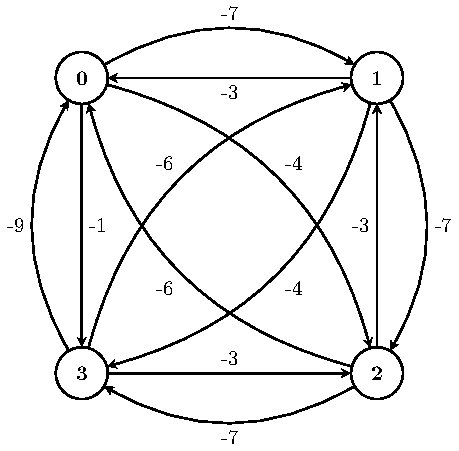
\includegraphics[scale=1.1]{graphs/salesman-example.pdf}
	\centering
\end{figure}

Find a Hamiltonian cycle with minimum cost. 

First of all, let us take a deeper look into our possible solutions. There are $(n-1)!$ cycles in a graph with $n$ nodes. For our $4$-nodes graph there are $3! = 6$ type of cycles:

\begin{itemize}
	\item Type A: $0 \rightarrow 1 \rightarrow 2 \rightarrow 3 \rightarrow 0$
	\item Type B: $0 \rightarrow 3 \rightarrow 2 \rightarrow 1 \rightarrow 0$
	\item Type C: $0 \rightarrow 2 \rightarrow 1 \rightarrow 3 \rightarrow 0$
	\item Type D: $0 \rightarrow 3 \rightarrow 1 \rightarrow 2 \rightarrow 0$
	\item Type E: $0 \rightarrow 1 \rightarrow 3 \rightarrow 2 \rightarrow 0$
	\item Type F: $0 \rightarrow 2 \rightarrow 3 \rightarrow 1 \rightarrow 0$
\end{itemize}

We may see this graphically in table \ref{tbl:salesman-cycles}.

\begin{table}[H]
	\centering
	\begin{tabular}{ccc}		
		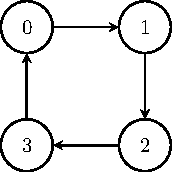
\includegraphics[scale=.9]{graphs/salesman-cycleA.pdf} &
		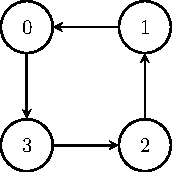
\includegraphics[scale=.9]{graphs/salesman-cycleB.pdf} &
		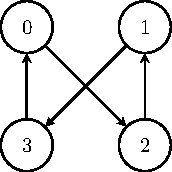
\includegraphics[scale=.9]{graphs/salesman-cycleC.pdf} \\
		
		Type A & Type B & Type C \\
		
		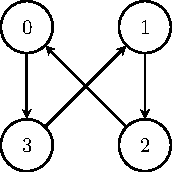
\includegraphics[scale=.9]{graphs/salesman-cycleD.pdf} &
		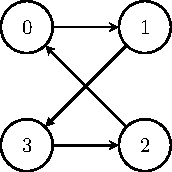
\includegraphics[scale=.9]{graphs/salesman-cycleE.pdf} &
		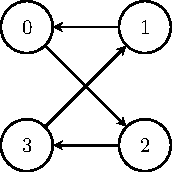
\includegraphics[scale=.9]{graphs/salesman-cycleF.pdf} \\
		
		Type D & Type E & Type F \\
	\end{tabular}
	\caption{Type of cycles in a $4$-nodes graph}
	\label{tbl:salesman-cycles}
\end{table}

These six are the only possible cycles through our graph and one of them will have minimum cost. Since our binary encoding additionally depends on the node position, there are $4$ solutions of our encoding that represent the same cycle. For example, ($0 \rightarrow 1 \rightarrow 2 \rightarrow 3 \rightarrow 0$) and ($1 \rightarrow 2 \rightarrow 3 \rightarrow 0 \rightarrow 1$) both represent cycle type A. In this case, type A will be the tour with minimum cost.

A graphical representation of the different penalties interactions is shown in figure \ref{fig:salesman-penalties}, based on the constraints defined above.

\begin{table}[H]
	\centering
	\makebox[\textwidth][c]{
		\begin{tabular}{ccc}		
			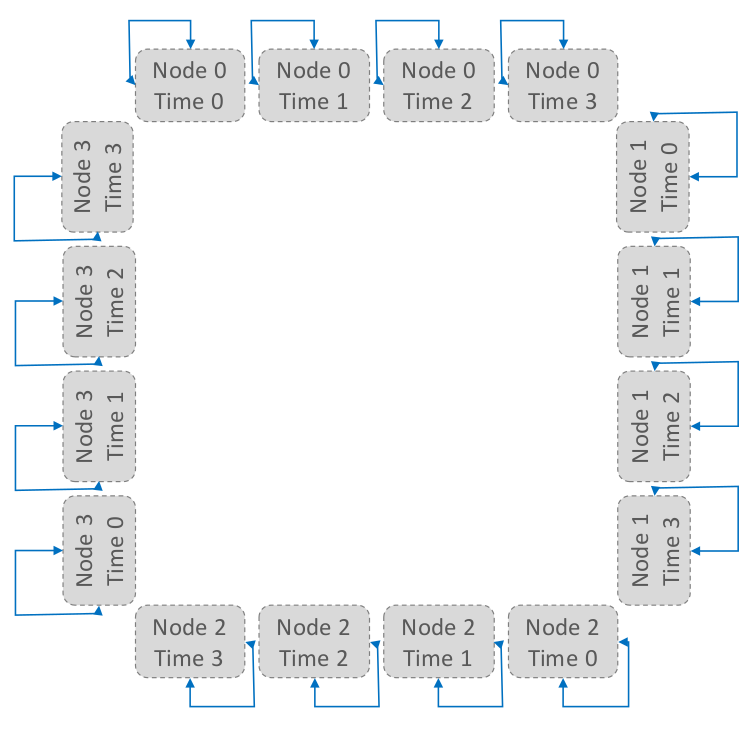
\includegraphics[scale=0.2]{salesman-penalties1.png} &
			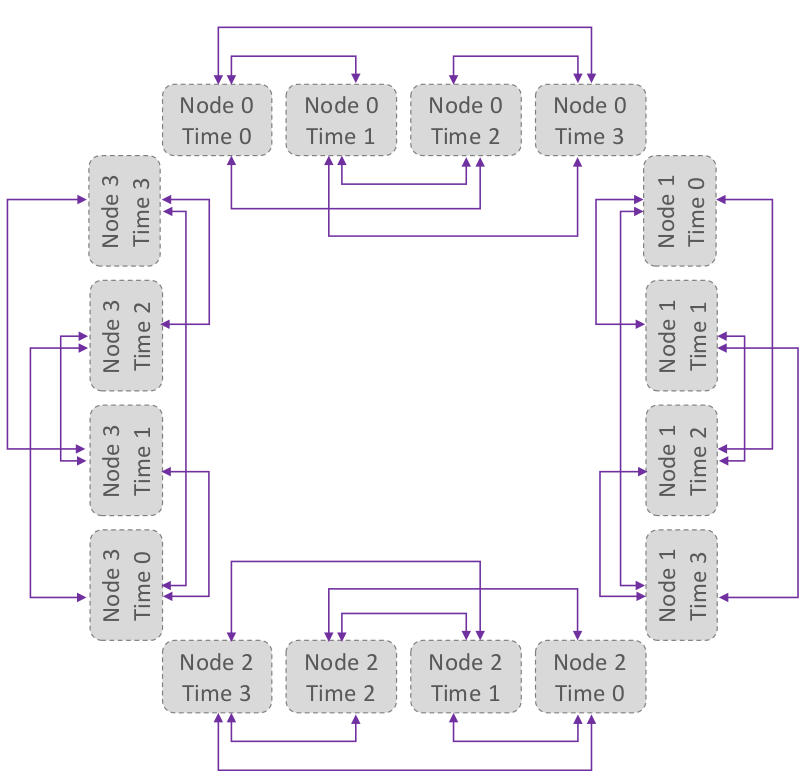
\includegraphics[scale=0.2]{salesman-penalties2.png} &
			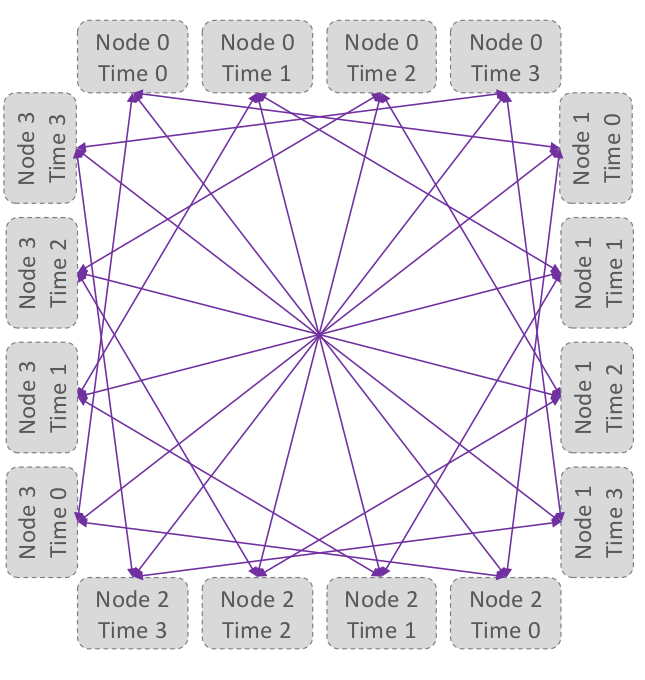
\includegraphics[scale=0.2]{salesman-penalties3.png} \\
			
			1: Self-bias & 2: Repetition & 3: Colocation \\
			
			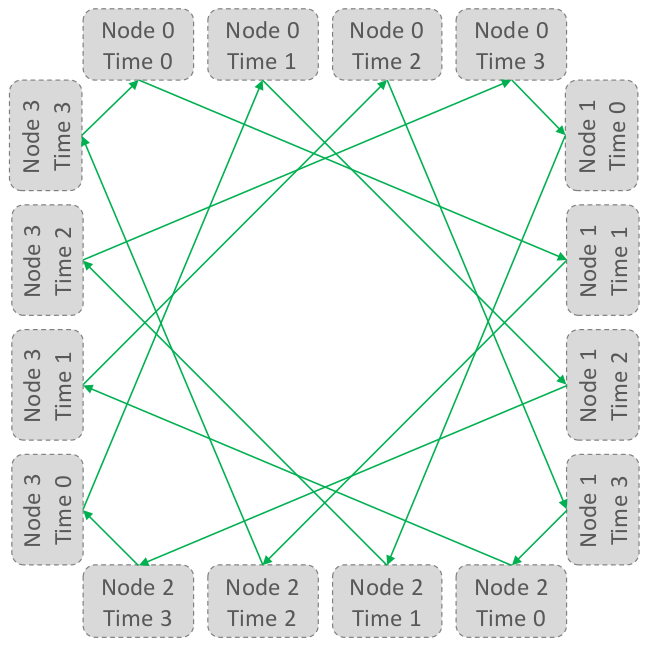
\includegraphics[scale=0.2]{salesman-penalties4.png} &
			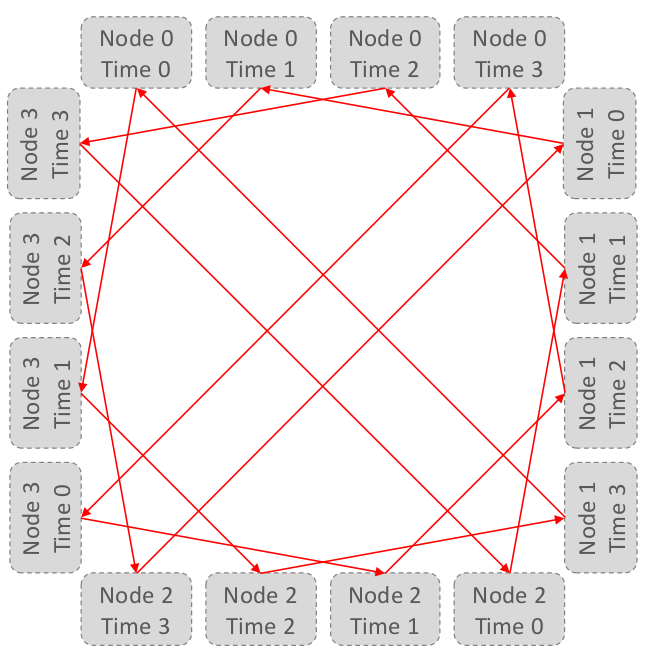
\includegraphics[scale=0.2]{salesman-penalties5.png} &
			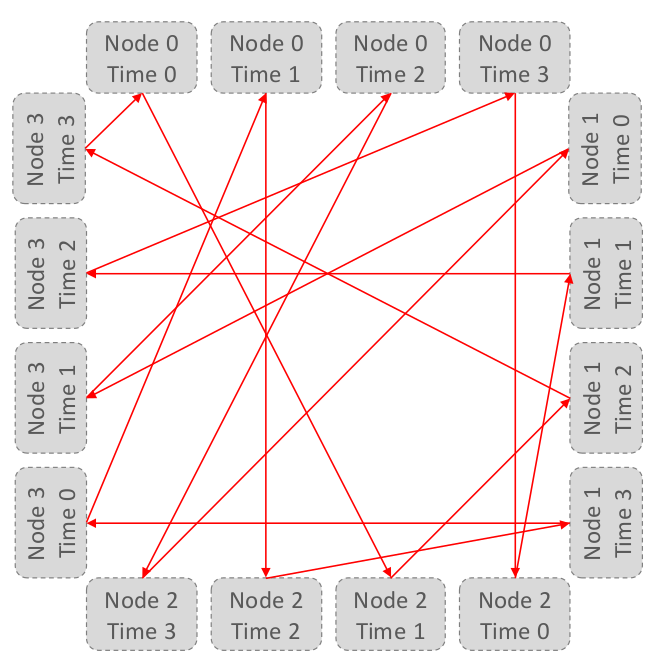
\includegraphics[scale=0.2]{salesman-penalties6.png} \\
			
			4: Type A tours & 5: Type B tours & 6: Type C tours \\
			
			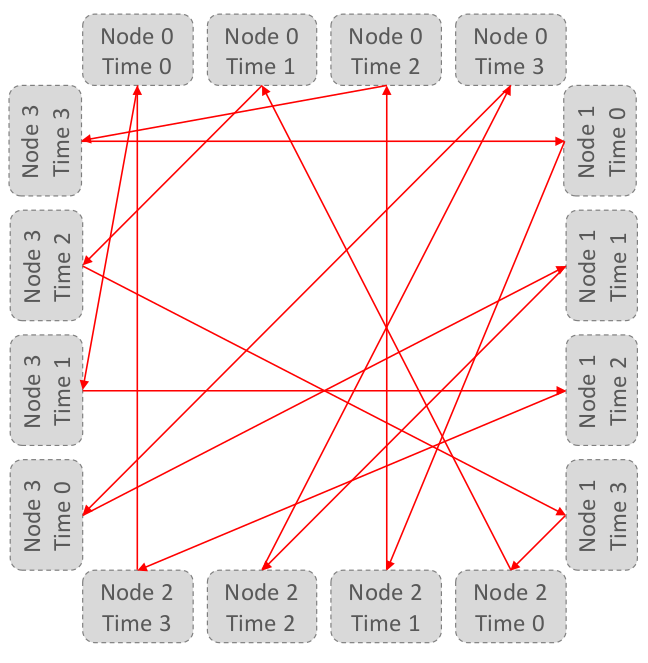
\includegraphics[scale=0.2]{salesman-penalties7.png} &
			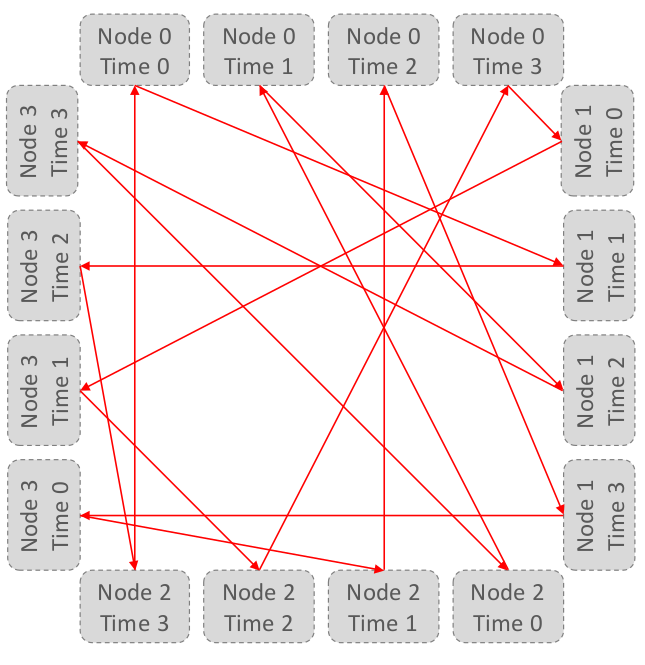
\includegraphics[scale=0.2]{salesman-penalties8.png} &
			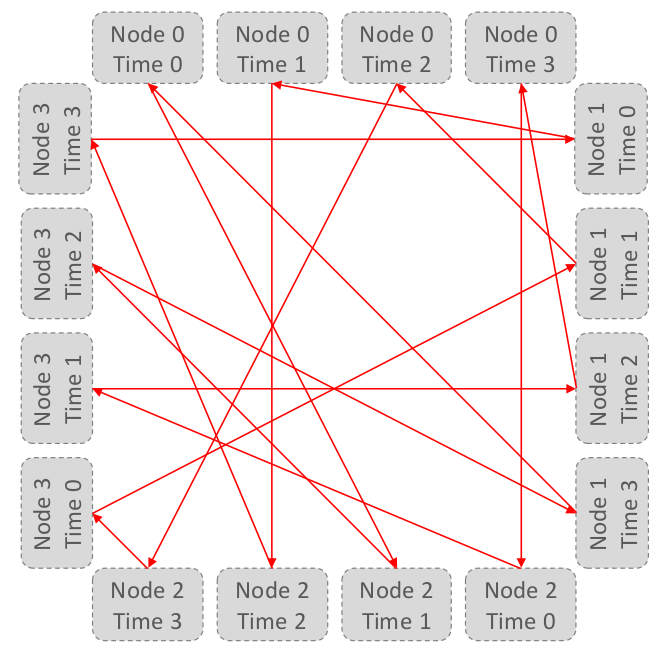
\includegraphics[scale=0.2]{salesman-penalties9.png} \\
			
			7: Type D tours & 8: Type E tours & 9: Type F tours \\
		\end{tabular}
	}
	\caption{Graphical representation of penalties between interactions \cite{Sarkar2020}}
	\label{fig:salesman-penalties}
\end{table}

We start the problem refactoring by renaming the variables:

$$ (x_{0,0}, x_{0,1}, x_{0,2}, x_{0,3}, x_{1,0}, x_{1,1}, x_{1,2}, \dots, x_{3,2}, x_{3,3}) =
(x_1, x_2, x_3, x_4, x_5, x_6, x_7, \dots, x_{15}, x_{16}) $$

\begin{figure}[H]
	\makebox[\textwidth][c]{
		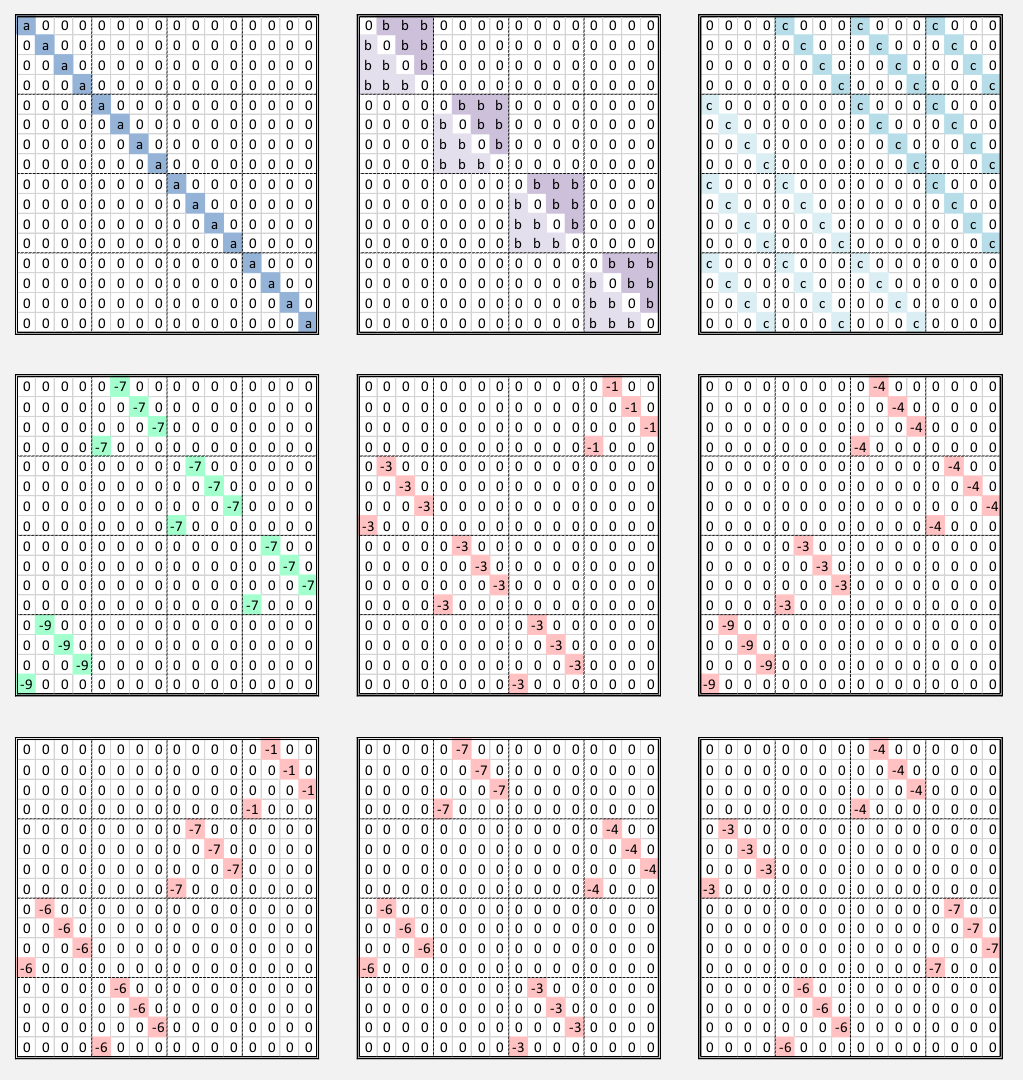
\includegraphics[scale=0.5]{salesman-adj-matrices.png}
	}
	\centering
	\caption{Term by term penalty matrices \cite{Sarkar2020}}
	\label{fig:salesman-adj-matrices}
\end{figure}

Each of the terms in the cost function \ref{eqn:salesman-cost-funct} may be transformed into a matrix. The term associated to the weights is additionally split using the different types of cycles in which they appear. We thus obtain nine adjacency matrices, found on figure \ref{fig:salesman-adj-matrices}.

Note that the matrices associated with the constraints are all symmetric. This happens because they only depend on the graph topology and not on the weights. On the other hand, since the cost of going back and forth between a pair of nodes is not the same, the matrices associated with the cycles are never symmetric.

The final $Q$ matrix for our problem is obtained by adding these matrices. Experimental evidence suggests that setting $a = 0$ and $b = c = 13$ and applying quantum annealing yields optimal solutions our the cost function \cite{Sarkar2020}. Using these values for the penalties, the final $Q$ matrix is seen in figure \ref{fig:salesman-Q-matrix}.

\begin{figure}[H]
	\makebox[\textwidth][c]{
		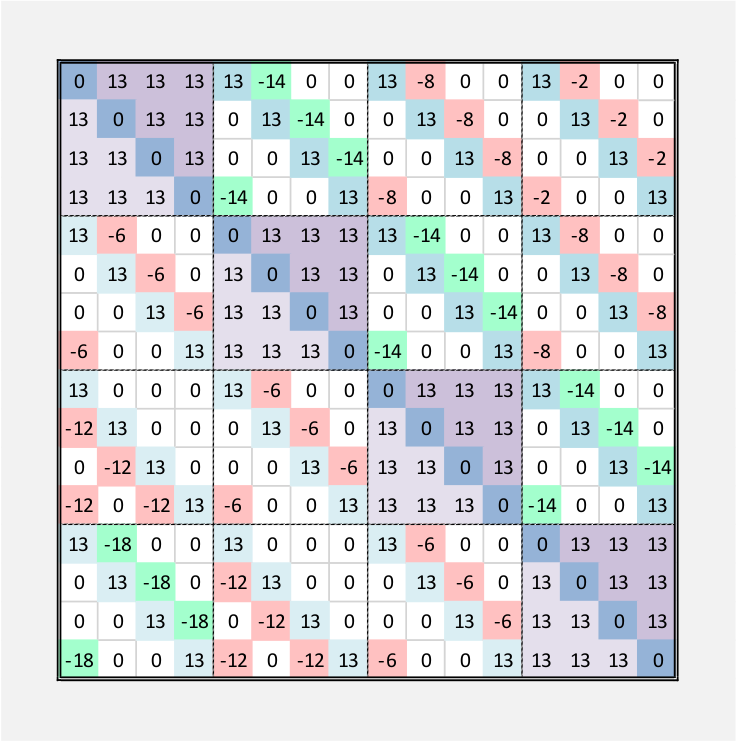
\includegraphics[scale=0.4]{salesman-Q-matrix.png}
	}
	\centering
	\caption{Final Q-matrix \cite{Sarkar2020}}
	\label{fig:salesman-Q-matrix}
\end{figure}

Finally transforming our problem into a QUBO in its matrix form, using the previous matrix:

$$ \text{Minimize } f(x) = x^T Q x $$

Finding one of the following minimas:

\begin{itemize}
	\item $x^T = [1000010000100001]$, equivalent to $x_{0,0} = x_{1,1} = x_{2,2} = x_{3,3} = 1$ and $0$ otherwise. Or in path notation: $(0 \rightarrow 1 \rightarrow 2 \rightarrow 3 \rightarrow 0)$
	\item $x^T = [0100001000011000]$, equivalent to $x_{0,1} = x_{1,2} = x_{2,3} = x_{3,0} = 1$ and $0$ otherwise. Or in path notation: $(1 \rightarrow 2 \rightarrow 3 \rightarrow 0 \rightarrow 1)$
	\item $x^T = [0010000110000100]$, equivalent to $x_{0,2} = x_{1,3} = x_{2,0} = x_{3,1} = 1$ and $0$ otherwise. Or in path notation: $(2 \rightarrow 3 \rightarrow 0 \rightarrow 1 \rightarrow 2)$
	\item $x^T = [0001100001000010]$, equivalent to $x_{0,3} = x_{1,0} = x_{2,1} = x_{3,2} = 1$ and $0$ otherwise. Or in path notation: $(3 \rightarrow 0 \rightarrow 1 \rightarrow 2 \rightarrow 3)$
\end{itemize}

Which corresponds to the four ways of encoding type A cycles with our notation.


\FloatBarrier
\section{D-Wave Systems}


\textbf{D-Wave Systems Inc.} is a Canadian company dedicated to quantum computing. In 2011, they announced the first commercial quantum computer system, D-Wave One. During the following two decades, the D-Wave team has developed a series of quantum computers dedicated to quantum annealing. The last one being the Advantage System (figure \ref{fig:advantage}).

\begin{figure}[h]
	\includegraphics[scale=.1]{advantage_system.png}
	\centering
	\caption{Advantage$^{TM}$ system}
	\label{fig:advantage}
\end{figure}

The quantum processing unit (QPU) of this system consists of $5640$ qubits and $40,484$ \emph{couplers} (links between qubits that allow entanglement between a pair of qubits). It can be seen in figure \ref{fig:QPU}. The number of couplers is especially relevant. A coupler is a physical mechanism that allows two qubits to be entangled. We will explain couplers in-depth in the next section. The different D-Wave architectures are explained in section \ref{sec:topologies}. In table \ref{tab:dwave-comp}, we see a comparison between the number of qubits and couplers from the different versions of the D-Wave computer system.

\begin{table}[h]
	\centering
	\makebox[\textwidth][c]{
		\begin{tabular}{cccccc}
							& D-Wave One 	& D-Wave Two	& D-Wave 2X 	& D-Wave 2000Q 	& Advantage \\ \hline
			Release date 	& May 2011	 	& May 2013 		& August 2015	& January 2017	& 2020   	\\
			Qubits 			& $128$	 		& $512$ 		& $1152$		& $2048$		& $5640$  	\\
			Couplers 		& $352$	 		& $1,472$ 		& $3,360$		& $6,016$		& $40,484$  
		\end{tabular}
	}
	\caption{D-Wave historical comparison \cite{DwaveWikipedia}}
	\label{tab:dwave-comp}
\end{table}

Since the QPU must be isolated to operate, it is encapsulated in a system at temperatures below 15 mK. In addition, radio frequency (RF)-shielded enclosure and magnetic shieldings are used to protect it from electromagnetic interference \cite{DWaveDoc}.

\begin{figure}[h]
	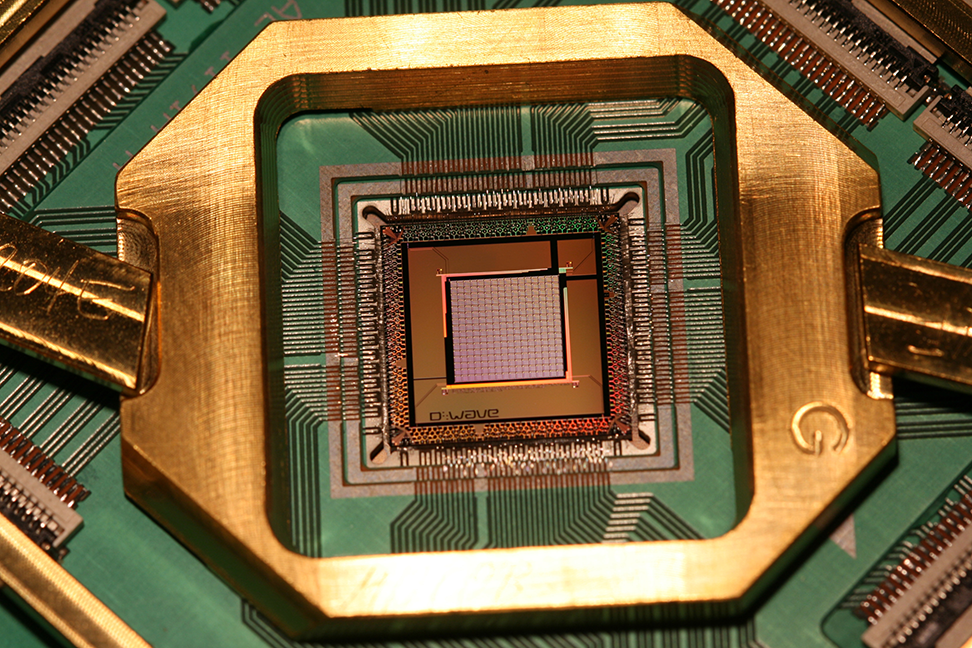
\includegraphics[scale=.2]{qpu.png}
	\centering
	\caption{D-Wave QPU}
	\label{fig:QPU}
\end{figure}

D-Wave provides an easy-to-use software environment to solve problems using quantum annealing. We will explain it in-depth in section [TODOref].


\subsection{Quantum Annealing in D-Wave}
\label{sec:quantum-annealing-dwave}


For this section, we refer to the D-Wave documentation, which explains how quantum annealing is implemented and may be exploited in the D-Wave systems \cite{DWaveDoc-QuantumAnnealing}.

Let us start by describing how qubits are physically implemented in D-Wave's QPU. Superconducting loops are used for this purpose, with a circulating current and a magnetic field. Depending on the direction of the current, the qubit will be in state $0$ or $1$; see figure \ref{fig:dwave-qubit}.

\begin{figure}[h]
	\makebox[\textwidth][c]{
		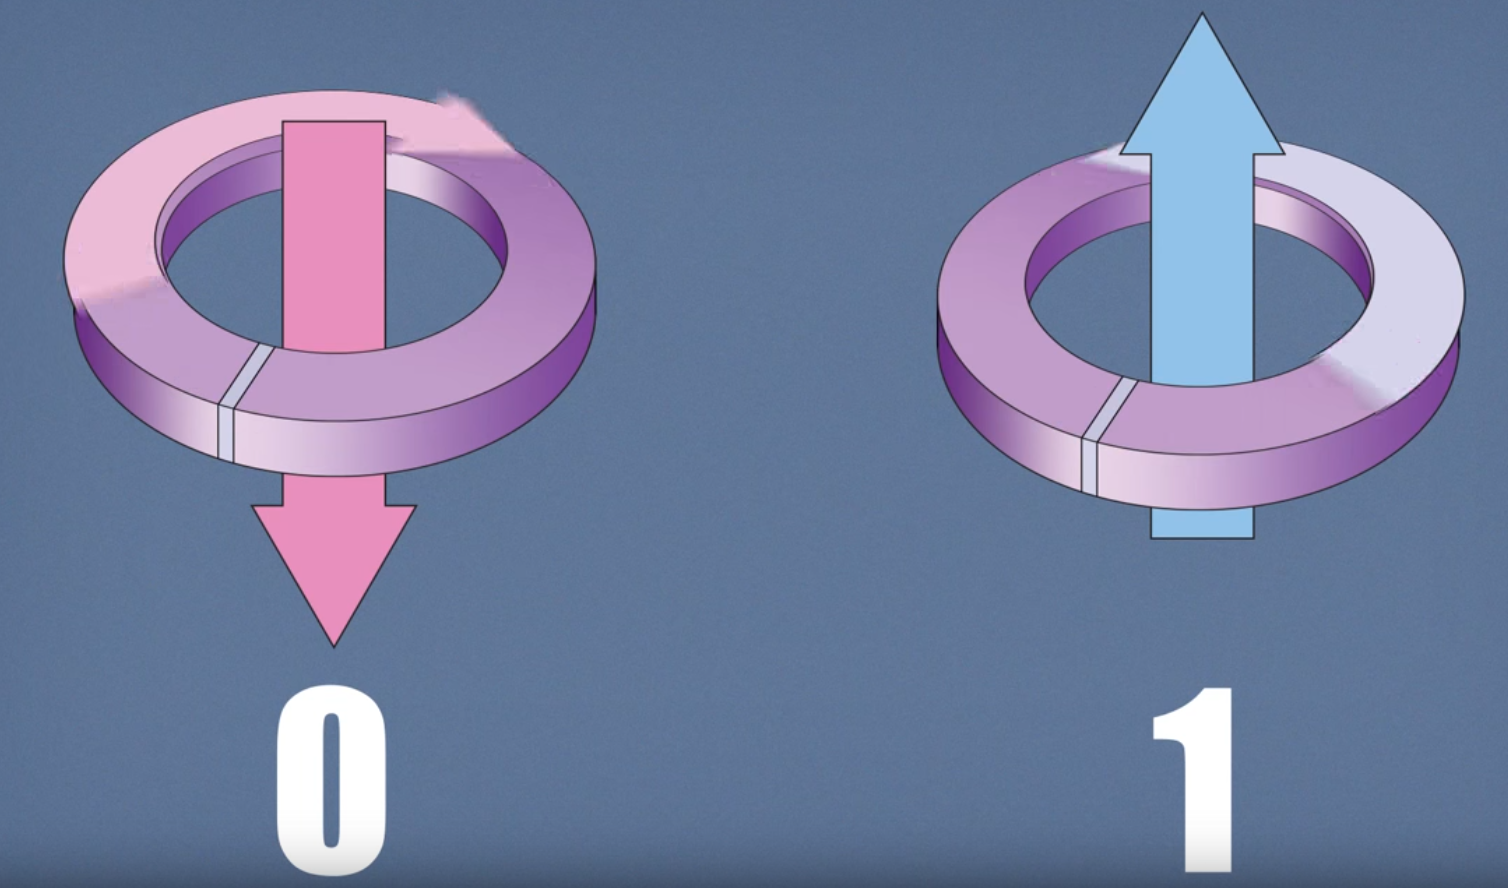
\includegraphics[scale=.2]{dwave-qubit.png}
	}
	\centering
	\caption{D-Wave's qubit, using a circulating current \cite{DWaveDoc-QuantumAnnealing}}
	\label{fig:dwave-qubit}
\end{figure}

In figure \ref{fig:dwave-annealing} we see a diagram with the evolution of a single qubit's energy during the annealing. By applying a magnetic field to the qubit we may affect the current and put the qubit in a superposition of both states (a). At this point, the energy is represented by a single valley with a single minimum: the superposition state where the qubit starts. Remember that at the end of the annealing we will measure every qubit and make them collapse to either one of those states, so we will never see a superposition in our measurements.

\begin{figure}[h]
	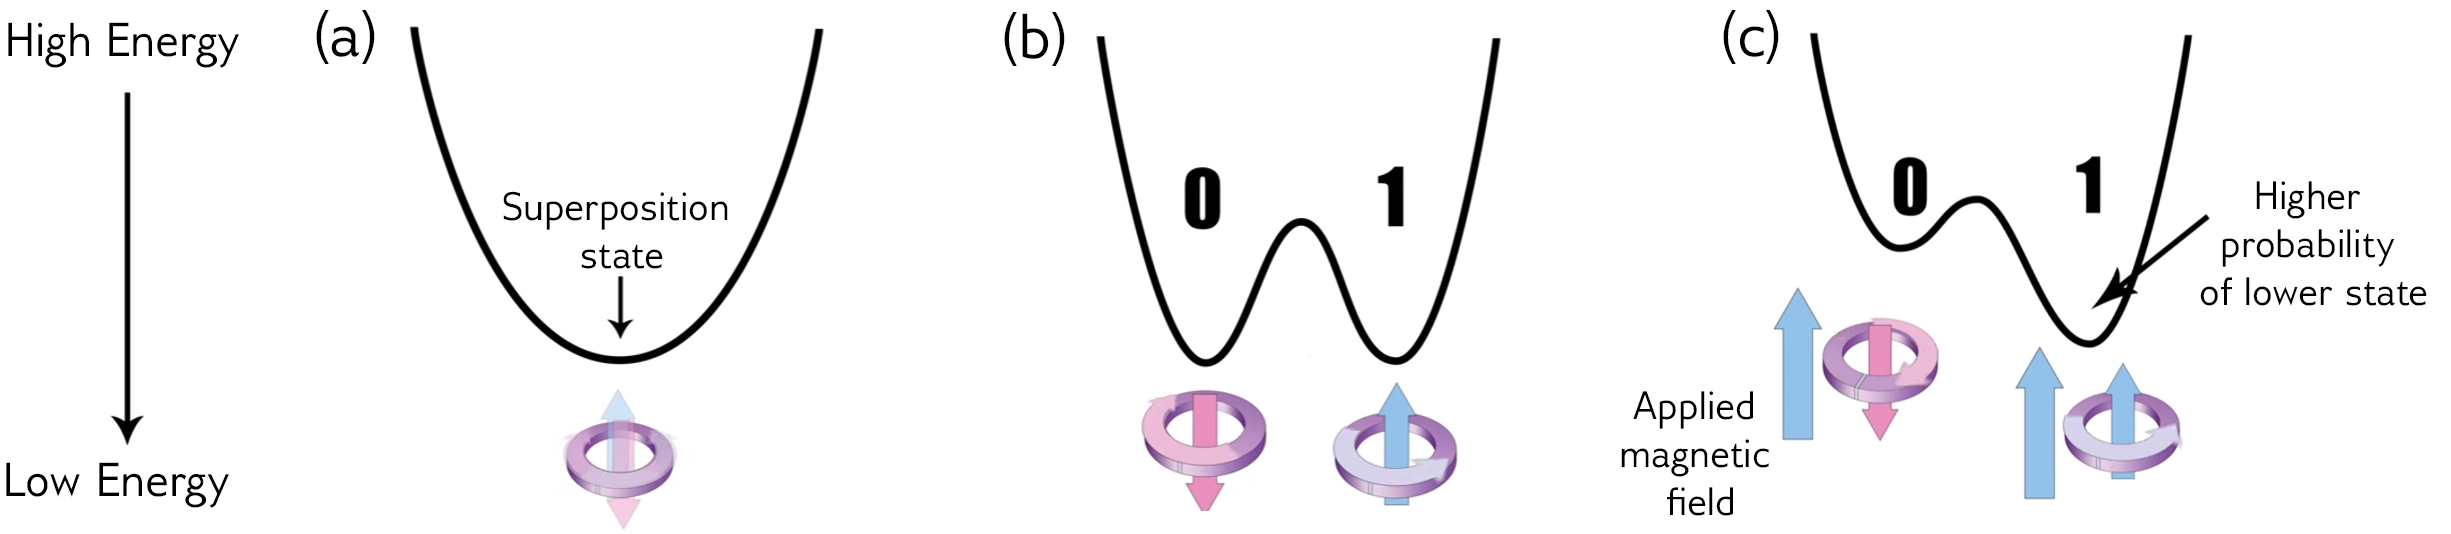
\includegraphics[scale=.2]{dwave-annealing.png}
	\centering
	\caption{Energy diagram changes upon running the annealing and applying bias \cite{DWaveDoc-QuantumAnnealing}}
	\label{fig:dwave-annealing}
\end{figure}

Then, the quantum annealing is run, turning the energy diagram into what is called a \emph{double well potential} (b). The lower point of the left valley corresponds to the $0$ state and the right one to the $1$ state. If we measured the qubit now, it would end up with equal probability in either one of both states. However, we may influence the qubit's energy by applying a magnetic field and tilting the double-well to one of the base states (c), increasing the probability of ending in that state. This new magnetic field is called \emph{bias} and the qubit minimizes the energy subject to the applied bias.

Biases applied on single qubits alone do not take full advantage of quantum annealing. We will also need \emph{couplers}, devices that entangle qubits to each other. A coupler can make two qubits tend to end in the same state or in opposite states with certain strength. As with bias, the coupler strength, usually called \emph{weight}  may be controlled by the programmer. Together the biases and the weights are the parameters that define a problem in the D-Wave system. As the reader may already imagine, these are the parameters of a QUBO / Ising model that we may define.

Consider a 2-qubits system for the following simple example. There will be three parameters: the 2 qubits biases and the coupler weight between them. As we know, two entangled qubits may be in four possible states: $(0,0)$, $(0,1)$, $(1,0)$ or $(0,0)$. The previous parameters define what is known as the \emph{energy landspace}. Figure \ref{fig:dwave-2qubit-landscape} illustrates this idea. The energy of each state depends on the biases and the single weight.

\begin{figure}[h]
	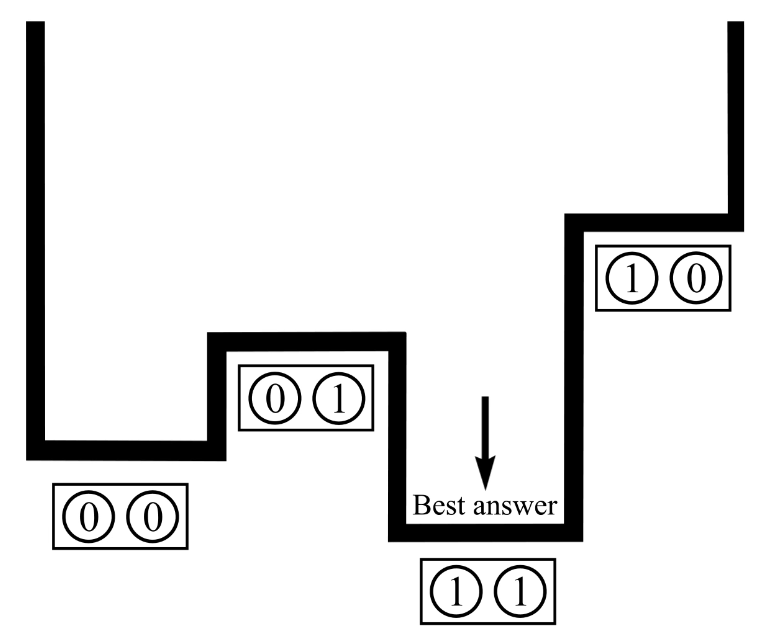
\includegraphics[scale=.25]{dwave-2qubit-landscape.png}
	\centering
	\caption{Example of 2-qubit energy landscape \cite{DWaveDoc-QuantumAnnealing}}
	\label{fig:dwave-2qubit-landscape}
\end{figure}

Let us take a look at the underlying quantum physics of this process. We make use of the Hamiltonian of a quantum system, which describes the evolution of the quantum system as per Postulate 3' [TODOref]. It maps the \emph{eigenstates} of the system to their energies. Only when the system is on an eigenstate, the energy of the system is well defined and called \emph{eigenenergy}, which are just the eigenvalues. The set of eigenstates and eigenenegies is called the \emph{eigenspectrum}. Recall that the lowest energy state is called the \emph{ground state}.

For a D-Wave system, the Hamiltonian may be described as:

$$ H(s) = \underbrace{- \frac{A(s)}{2} \bigg( \sum_i \upsigma_x^{(i)} \bigg)}_\text{Initial Hamiltonian} 
			+ \underbrace{\frac{B(s)}{2} \bigg( \sum_i h_i \upsigma_z^{(i)} + \sum_ {i > j} J_{i,j} \upsigma_z^{(i)} \upsigma_z^{(j)} \bigg)}_\text{Final Hamiltonian} $$

where $\upsigma^{(i)}_{x,z}$ are the Pauli matrices $X$ and $Z$ respectively operating on qubit $(i)$, $h_i$ are the qubit biases, and $J_{i,j}$ are the couplers weights.

As explained in the adiabatic evolution section \ref{sec:adiabatic-evolution}, the Hamiltonian is made of two terms:

\begin{itemize}
	\item The Initial Hamiltonian, also called \emph{tunneling Hamiltonian}, where the ground state is when every qubit is in superposition but no entanglement between qubit takes place.
	\item The Final Hamiltonian, also called \emph{problem Hamiltonian}, where the biases and weights are such that the ground state is the solution of the problem we are trying to solve.
\end{itemize}

In fact, the final Hamiltonian is precisely an Ising model. By expressing our problem as an Ising -or, equivalently, a QUBO- we may encode it inside this Hamiltonian using the parameters $h_i$ and $J_{i,j}$.

We may parametrize $s \in [0,1]$ as an abstract parameter that controls the annealing timing. Assuming the initial time is $t_0 = 0$, $s$ is defined as $s \equiv t / t_{final}$. Thus, the annealing occurs when $s$ goes from $0$ to $1$. We may define the annealing functions $A(s), B(s)$ such that $A(0) \gg B(0)$ and $A(1) \ll B(1)$. For instance, as seen in figure \ref{fig:dwave-annealing-functions}.

\begin{figure}[h]
	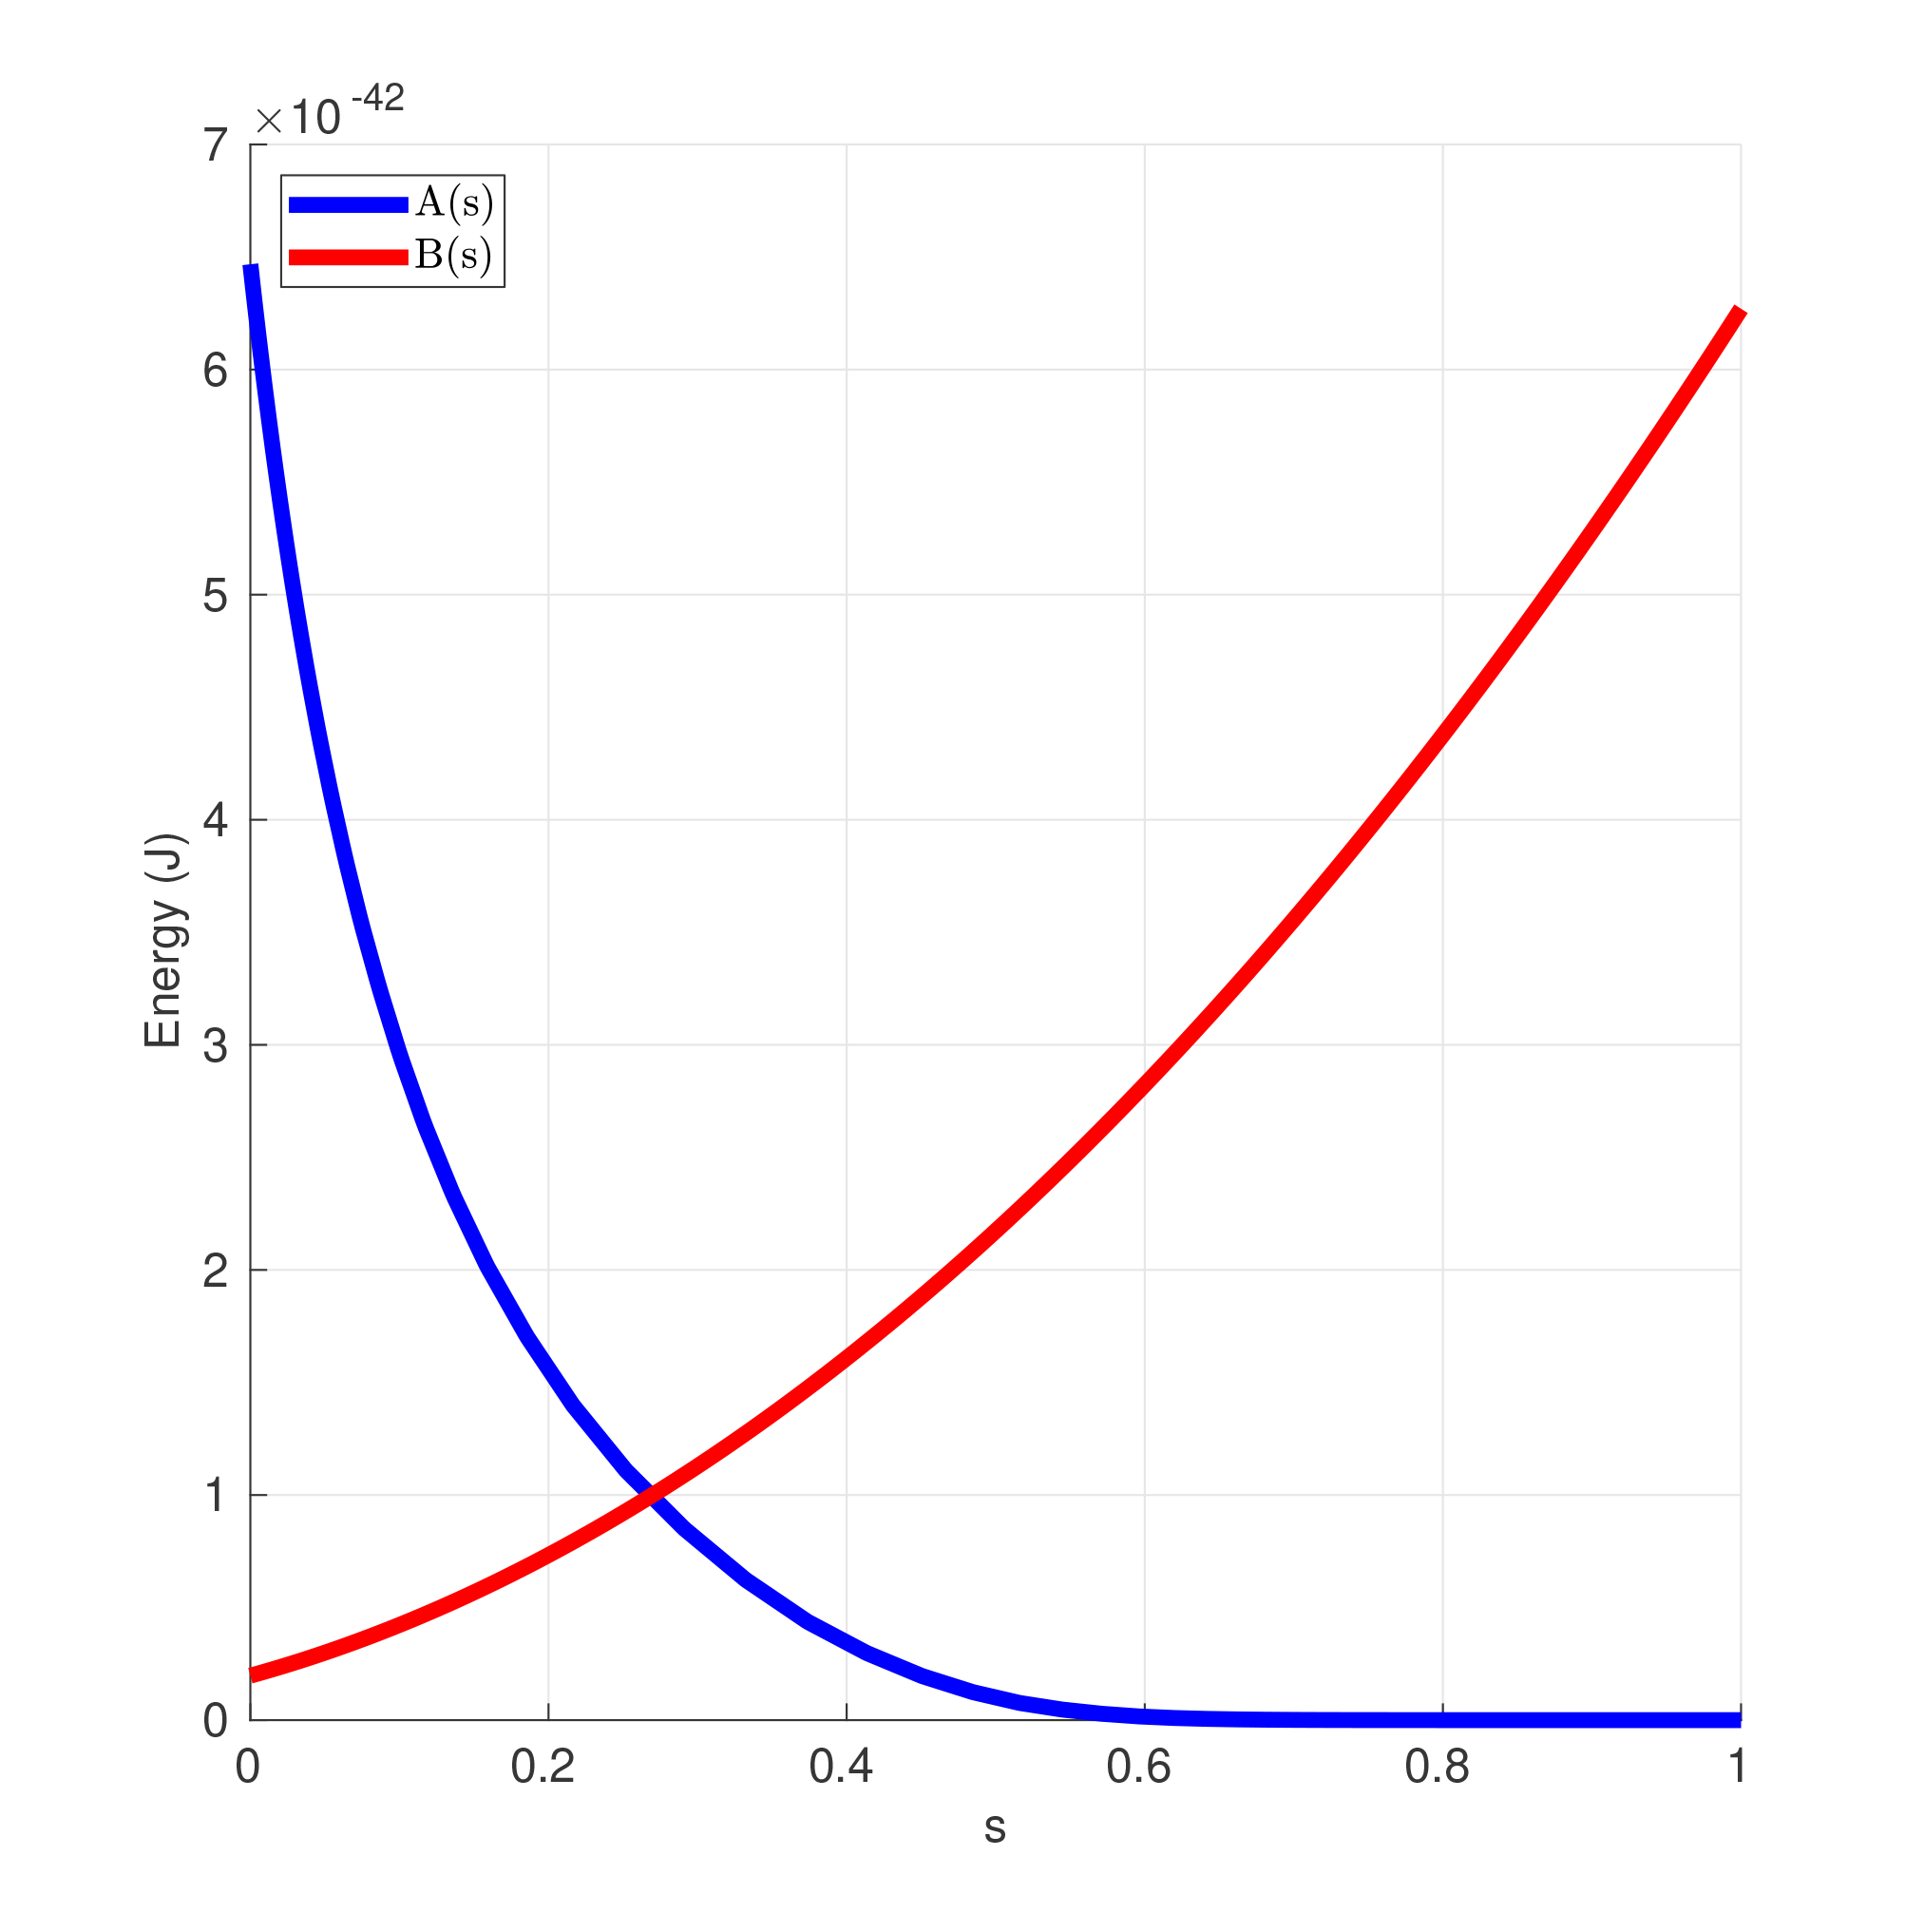
\includegraphics[scale=.14]{dwave-annealing-functions.png}
	\centering
	\caption{Annealing functions for the D-Wave 2X systems \cite{DWaveDoc-QuantumAnnealing}}
	\label{fig:dwave-annealing-functions}
\end{figure}

With these restrictions on the annealing functions, the system's Hamiltonian satisfies $H(0) = H_{initial}$ and $H(1) = H_{final}$. Therefore, the ground state at time $s=0$ matches the ground state of the initial Hamiltonian, and at time $t=1$, it matches the final Hamiltonian one. Under adiabatic evolution hypothesis, if the system starts in the initial Hamitolnian's ground state, it will end up in the final Hamiltonian one -which encodes the solution to our problem- at the end of the annealing.

The question remaining is, are the adiabatic evolution hypothesis met? We may control the time that the annealing takes by adjusting our annealing functions, a few microseconds are enough in most cases, but the exact time that would make the annealing adiabatic is never known. The additional hypothesis of the adiabatic theorem (\ref{th:adiabatic-theorem}) mentions the gap between the ground energy and the rest of eigenenergies. Let us look at a visual representation of the evolution of the eigenenergies of a given system against time in figure \ref{fig:dwave-eigenspectrum}.

\begin{figure}[h]
	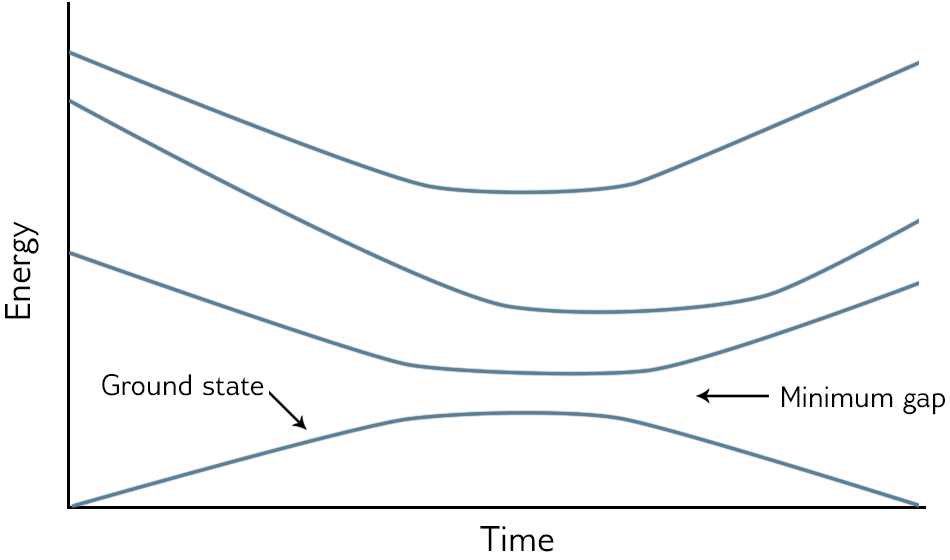
\includegraphics[scale=.3]{dwave-eigenspectrum.png}
	\centering
	\caption{Example of eigenspectrum evolution \cite{DWaveDoc-QuantumAnnealing}}
	\label{fig:dwave-eigenspectrum}
\end{figure}

The ground energy is plotted at the bottom. While the eigenenergies are far (the minimum gap holds), the probability of the system state jumping to another eigenstate is really low. When time elapses, the ground energy gets increasingly closer to the rest of the eigenenergies. The closer those energies are, the higher the probability of the system state jumping gets too. For every problem, there is a different Hamiltonian and, consequently, a different corresponding eigenspectrum. Generally, the most difficult problems for quantum annealing are those with really small minimum gaps.

In practice, these jumps may occur due to certain factors like thermal fluctuations or running the annealing process too quickly. Either way, a complete adiabatic process in the real world would mean perfect isolation, which is impossible. For some problems, the probability of staying in the ground state is really low, although low-energy states are also useful since they are associated to solutions with a low value in our cost function.


\subsection{D-Wave's QPU Topologies}
\label{sec:topologies}


In table \ref{tab:dwave-comp}, we saw the number of qubits and couplers of each one of the D-Wave QPUs. These QPUs implement a graph topology where the nodes are qubits and the couplers are the edges connecting two nodes together. However, a complete $n$-nodes graph has $n(n-1)$ nodes, and none of the D-Wave QPUs have as many couplers. For instance, the D-Wave 2000Q has $2048$ qubits and $6016$ couplers, far from the $2048 * 2047 = 4,192,256$ edges that it could have. Let us explore the graph topology underneath these systems in order to understand their problems and how to work around them.

There are two different topologies being used in the D-Wave systems. The \emph{Chimera} topology was used up until the D-Wave 2000Q system, include; while the \emph{Pegasus} topology is only in the recent Advantage system. 

In the \textbf{Chimera topology}, qubits are 'oriented' either horizontally or vertically, as seen in figure \ref{fig:chimera}.

\begin{figure}[h]
	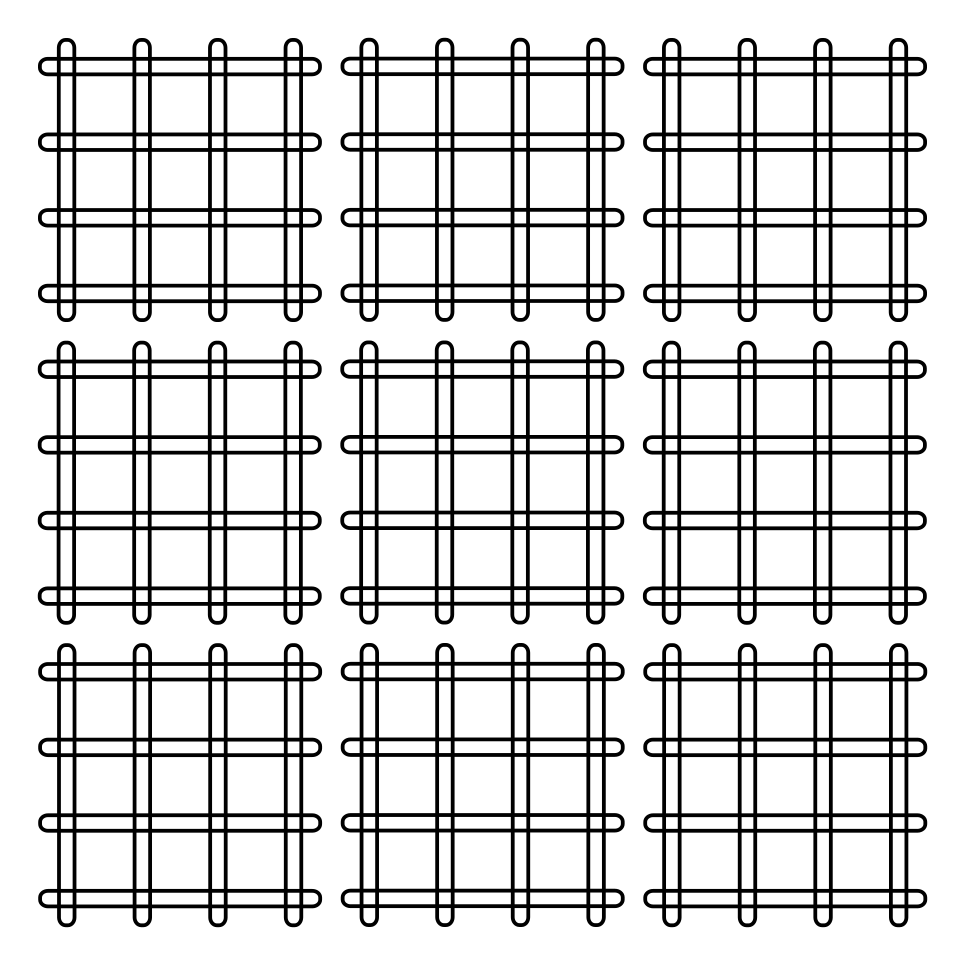
\includegraphics[scale=.3]{chimera.png}
	\centering
	\caption{Qubits represented as horizontal and vertical loops. This graphic shows three rows of 12 vertical qubits and three columns of 12 horizontal qubits for a total of 72 qubits, 36 vertical and 36 horizontal. \cite{DWaveDoc-Architecture}}
	\label{fig:chimera}
\end{figure}

For this topology it is conceptually useful to split couplers into two categories: Internal and external couplers. The \textbf{internal couplers} connect pair of orthogonal qubits. For example, in figure \ref{fig:chimera-internal-couplers} we see a green qubit connected to four black qubits through internal couplers.

\begin{figure}[H]
	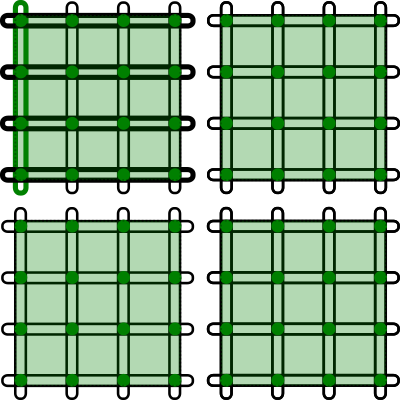
\includegraphics[scale=.5]{chimera-internal-couplers.png}
	\centering
	\caption{Internal couplers, represented as green dots at the intersections between qubits \cite{DWaveDoc-Architecture}}
	\label{fig:chimera-internal-couplers}
\end{figure}

The Chimera topology has a repetitive structure where sets of $4$ by $4$ qubits are grouped together. These are the translucent green squares in figure \ref{fig:chimera-internal-couplers} and are called \emph{unit cells}.

A unit cell can also be represented either as a cross or a column, as shown in figure \ref{quimera-unit-cell}. They are $K_{4,4}$ bipartite graphs. Meaning, there are two sets of $4$ qubits, qubits on a given set are connected to every qubit in the opposite set and have no more connections. same set but are connected to every qubit of the other one. For example, the green qubit labeled as $0$ is connected to all the nodes from the opposing set: $(4,5,6,7)$.

\begin{figure}[h]
	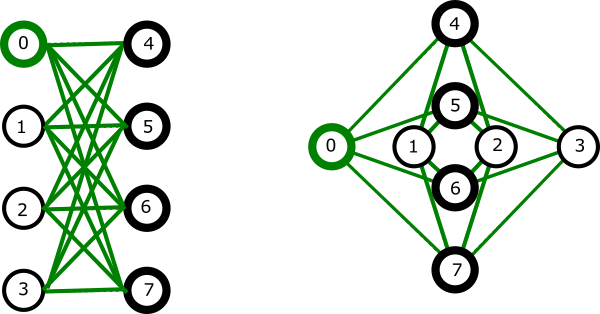
\includegraphics[scale=.7]{chimera-unit-cell.png}
	\centering
	\caption{Chimera unit cells \cite{DWaveDoc-Architecture}}
	\label{fig:chimera-unit-cell}
\end{figure}

The \textbf{external} couplers connect pairs of qubits in the same row or column, but from different unit cells. For example, in figure \ref{fig:chimera-external-couplers} the green qubit in the center unit cell is connected to the two blue qubits in other unit cells and two four black qubits in the same unit cell.

\begin{figure}[h]
	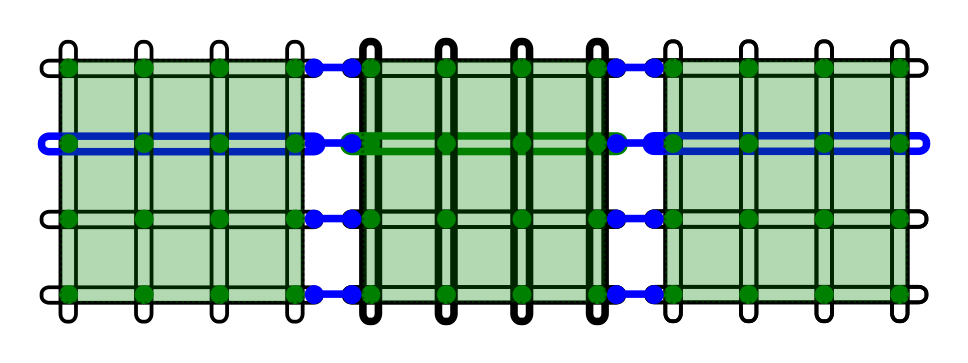
\includegraphics[scale=.5]{chimera-external-couplers.png}
	\centering
	\caption{External couplers, represented as blue connections between qubits \cite{DWaveDoc-Architecture}}
	\label{fig:chimera-external-couplers}
\end{figure}

Chimera qubits have:

\begin{itemize}
	\item A \emph{nomial length} of $4$. That is, each qubit is connected to $4$ orthogonal qubits via internal couplers.
	\item A \emph{degree} of $6$. That is, is qubit is connected to a total of $6$ other qubits.
\end{itemize}

The $K_{4,4}$ unit cells are connected by external couplers forming what is called a lattice. For instance, figure \ref{fig:chimera-extended} shows four connected unit cells that are part of a bigger topology. The notation $C_n$ refers to a chimera grid with an $N \times N$ grid of unit cells. Figure \ref{fig:chimera-internal-couplers} shows a $C_2$. The D-Wave 2000Q QPU supports a $C_16$ chimera graph.

\begin{figure}[h]
	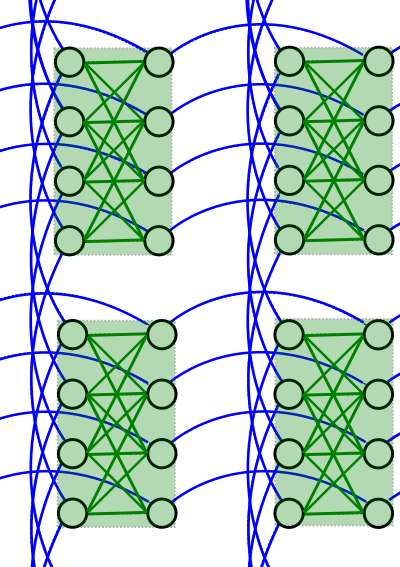
\includegraphics[scale=.4]{chimera-extended.png}
	\centering
	\caption{Cropped view of four unit cells, part of a bigger Chimera graph \cite{DWaveDoc-Architecture}}
	\label{fig:chimera-extended}
\end{figure}

The \textbf{Pegasus topology} is also organized in horizontal and vertical qubits, but they are shifted, as shown in figure \ref{fig:pegasus}. Conceptually, the chimera and the pegasus topology are not that different: the graph is divided into unit cells, connected between them using external couplers. However, a new kind of coupler is introduced in the Pegasus topology: the odd coupler.

\begin{figure}[h]
	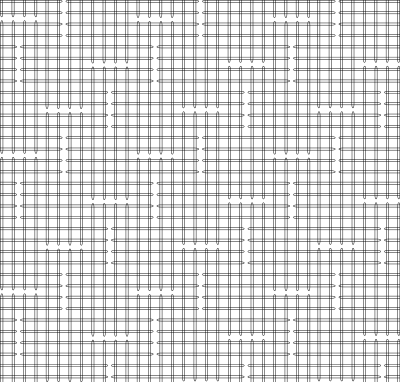
\includegraphics[scale=.08]{pegasus.png}
	\centering
	\caption{Pegasus graph \cite{DWaveDoc-Architecture}}
	\label{fig:pegasus}
\end{figure}

We will not deepen anymore into the Pegasus graph structure. It suffices to know that pegasus qubits have a nominal length of $12$ (each qubit is connected to $12$ orthonormal qubits using internal couplers) and a total degree $15$. A Pegasus cell contains $24$ qubits. Additionally, $P_n$ represents a Pegasus topology with an $N \times N$ grid of unit cells. The Advantage system supports a $P_{16}$ Pegasus graph.

Then, what are the disadvantages of these topologies? Consider a simple example with three binary variables $(a, b, c)$: find a configuration for the variables such that $a + b + c = 1$.

This simple satisfability problem can be transform using the energy function $E(x) = (1 - a - b - c)^2$, or equivalenty $E(x) = 2ab + 2ac + 2bc - a - b - c + 1$. This matches the following QUBO model:

$$ \text{Minimize } E(x) = x^T Q x + 1$$

where

$$
Q = 
\left(
\begin{array}{ccc}
	-1 & 1 & 1  \\
	1 & -1 & 1  \\
	1 & 1 & -1
\end{array}
\right), \quad
x = 
\left(
\begin{array}{c}
a  \\
b  \\
c
\end{array}
\right)
$$

This can be seen as the graph in figure \ref{fig:example-embedding}. Suppose we want to use a Chimera topology to solve this problem. The remaining question is how to embed this graph into a chimera unit cell such as \ref{fig:chimera-unit-cell-cross}. 

\begin{figure}[H]
	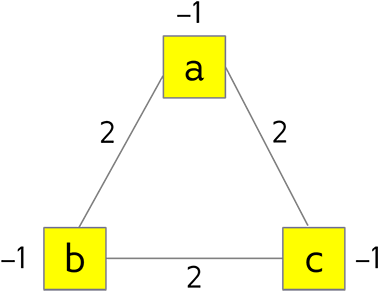
\includegraphics[scale=.3]{example-embedding.png}
	\centering
	\caption{Graph associated to QUBO model \cite{DWaveDoc-MinorEmbedding}}
	\label{fig:example-embedding}
\end{figure}

\begin{figure}[H]
	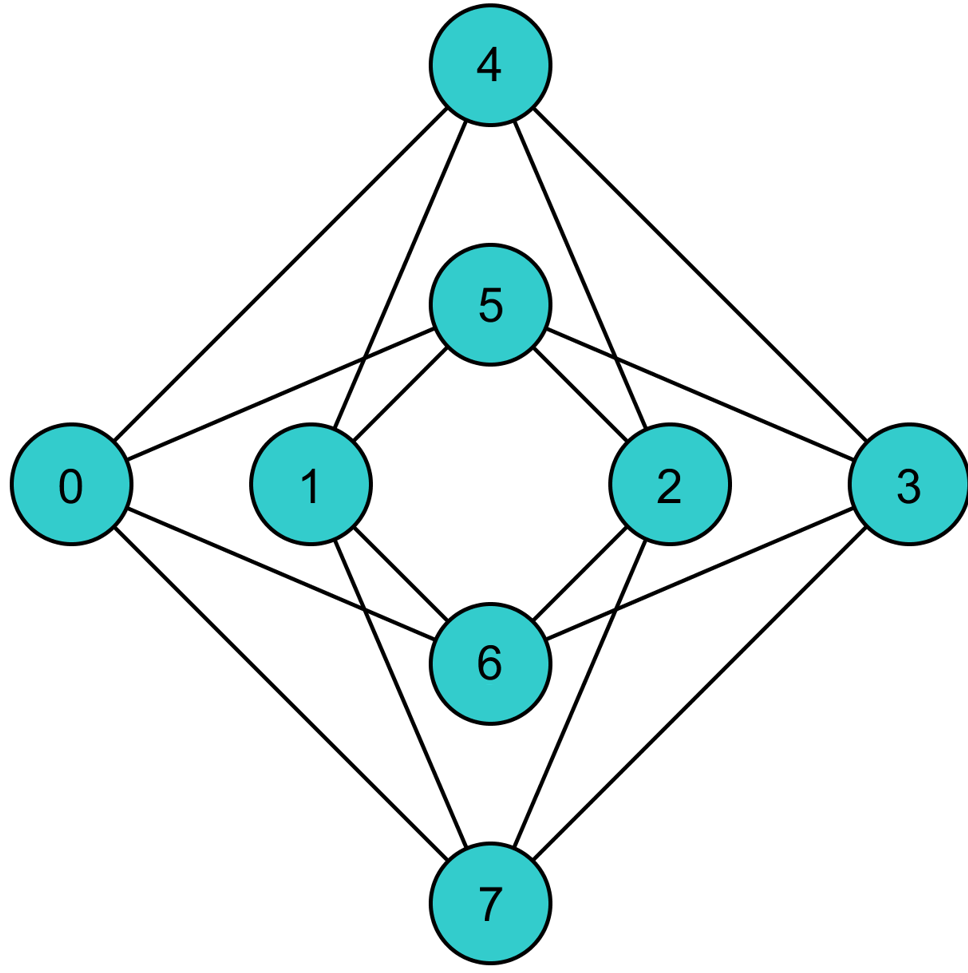
\includegraphics[scale=.2]{chimera-unit-cell-cross.png}
	\centering
	\caption{Chimera unit cell \cite{DWaveDoc-MinorEmbedding}}
	\label{fig:chimera-unit-cell-cross}
\end{figure}

However, there are no three nodes in a bipartite graph that form a triangle, so a direct embedding is not possible. Instead, a \emph{chain} is used: adjacent qubits are group together and conceptually assigned to a single node of our QUBO model graph. This process is shown in figure \ref{fig:embedding}. In practice, the coupler between qubits in a chain is set to a great negative value so the probability of both qubits ending up in the same state is really high. We will never manually embed a graph since D-Wave provides an automatic way of computing an (at least) suboptimal embedding.

\begin{figure}[H]
	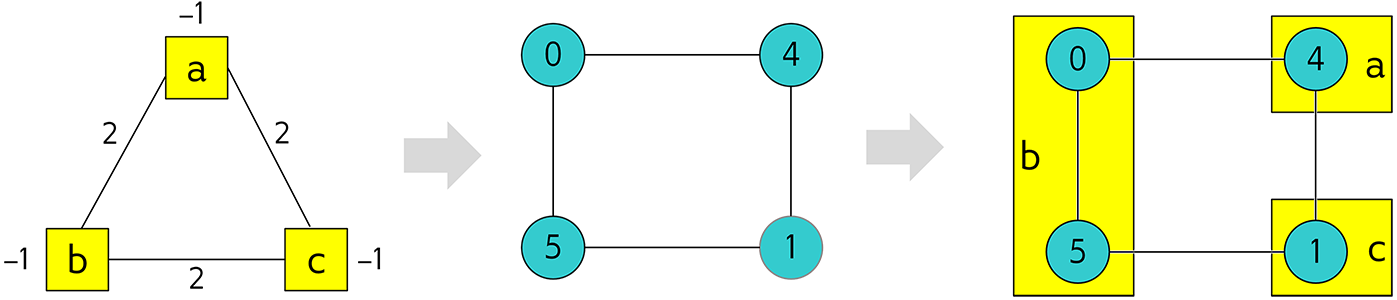
\includegraphics[scale=.3]{embedding.png}
	\centering
	\caption{Embedding process \cite{DWaveDoc-MinorEmbedding}}
	\label{fig:embedding}
\end{figure}

\chapter{Solving the De Novo Genome Assembly}


In this last chapter, we approach the genome assembly problem with the use of quantum annealing. Let us first understand what this problem is, and then translate it to a QUBO model and solve it using quantum annealing.


\section{The Genome Assembly Problem}


The genome of an organism is all its genetic material \cite{Roth2019}. The deoxyribonucleic acid (DNA) is the carrier of that genetic information. It consists of two long chains twisted to form a double helix \cite{Alberts2007}. Each of these chains is composed of a series of nucleotides or bases: adenine (A), guanine (G), cytosine (C), and thymine (T). Since these bases are matched in pairs in the DNA double helix, they are called base pairs (bp).

A genome sequence is the complete list of nucleotides of every chromosome of an organism. With today's technology, automated sequence machines can read up to $10.000$ bp at a time \cite{Reinert1015} while the human genome contains 3 Mbp, so we cannot simply read the whole genome. This is where genome assembly comes in.

Genome assembly refers to the process of, given a large number of short DNA reads, stitch them together to form a large representation of the original chromosome where the reads came from. The two main techniques used to reconstruct these sequences are the ab initio reference-free alignment and the de novo reference-based assembly.


\subsection{Ab initio reference-based alignment}


In this method, the DNA reads are matched against a known trusted reference of the same organism. This is essentially a pattern matching problem, where we find the index of a given sub-string in a larger string. However, after the reconstruction is complete the result is compared to the reference in order to identify implications; therefore introducing bias based on the reference \cite{Sarkar2020}.

In the naive approach, the short sub-string is compared to the reference starting at the first index. If the end of the sub-string is reached with a positive, a match is obtained. Otherwise, the sub-string is shifted a single position and we compare again. Heuristic methods that improve on this idea are based on shifting a greater number of spaces after a mismatch.

Different number of strategies have been developed in this direction. For instance, the classic Boyer-Moore and Knuth-Pratt-Morris algorithms \cite{Holmes1999}. However, these in particular are not adequate for genome assembly since these are exact string matching algorithms and DNA reads usually need approximate matches due to reads errors. Other algorithms worth mentioning are the Needleman-Wunsch algorithm \cite{Needleman1970} and the Smith-Waterman algorithm \cite{Smith1981}, for global and local alignment respectively. These are dynamic programming algorithms designed specifically with DNA reads in mind. 

State of the art algorithms trades off accuracy for speed and memory. Given enough computational power, the de novo reference-free method yields better results without introducing any reference bias.


\subsection{De novo reference-free assembly}
\label{sec:de-novo-genome-assembly}

On the other hand, the de novo reference-free method is, as its name suggests, reference free. Meaning, it is based only on the DNA reads. Thus, it has no reference bias but it is more computationally complex. It is usually used the first time a species DNA is read.

In this technique, multiple copies of the same DNA are made before slicing it. After chopping each copy at random places the data is redundant and the different reads overlap, making the assembly easier. There are multiple methods for de novo assembly based on different tools: Overlap-Layout Consensus (OLC) methods, de Bruijn graph (DBG) methods, string graphs, greedy and hybrid methods are some of the most famous examples (for a review see \cite{Sohn2018}). Depending on the reading method and the number and length of the DNA reads, different methods excel from the rest. For instance, short-read technologies with a large number of reads favor DBG methods while high-quality long reads favor OCL methods. For our purposes, we will focus on the OCL method.

In the OLC graph used for the de novo whole-genome assembly, each node represents a different DNA read. Directed edges are associated a weight depending on how well these two reads are stitched together in a certain order. For example, the directed edge going from reading $r_1$ to read $r_2$ will be assigned a weight depending on how well $r_1r_2$ can be stiched.

The weights computation depends on the implementation. For the purpose of this thesis, we will use exact matches, no taking reading errors into consideration. Then, the weight assigned to an edge is the length of the overlap between both reads without any errors, with a change of sign. For example, given the reads $r_1 = AATT$ and $r_2 = TTCC$, the perfect stitching will produce $AATTCC$, so the overlap between both reads is $2$, giving a weight of $-2$. We may call this the \emph{distance} between reads $r_1$ and $r_2$ (in that order). It does not fulfill the mathematical definition of distance since it is not even symmetric, but it will be useful for us anyway.

A Hamiltonian path in our overlap graph will represent a series of reads in a certain order. By minimizing the total cost of our Hamiltonian path, we maximize the overlap between reads, resulting in the shortest possible final chain. This is exactly the same as solving the Travelling Salesman problem associated with our overlap graph.

Figure \ref{de-novo-process} shows the whole problem resolution \cite{Boev2020}. Given the DNA reads (a) we compute the overlap graph (b) using a distance between the reads. We continue by viewing this problem as a traveling salesman and transforming it into a QUBO model (c). Then, either a simulated annealer (e) or the D-Wave quantum annealer (d) are used to obtain the Hamiltonian path/cycle of minimum cost (f). Finally, we traverse the cycle and build the resulting genome sequence.

\begin{figure}[H]
	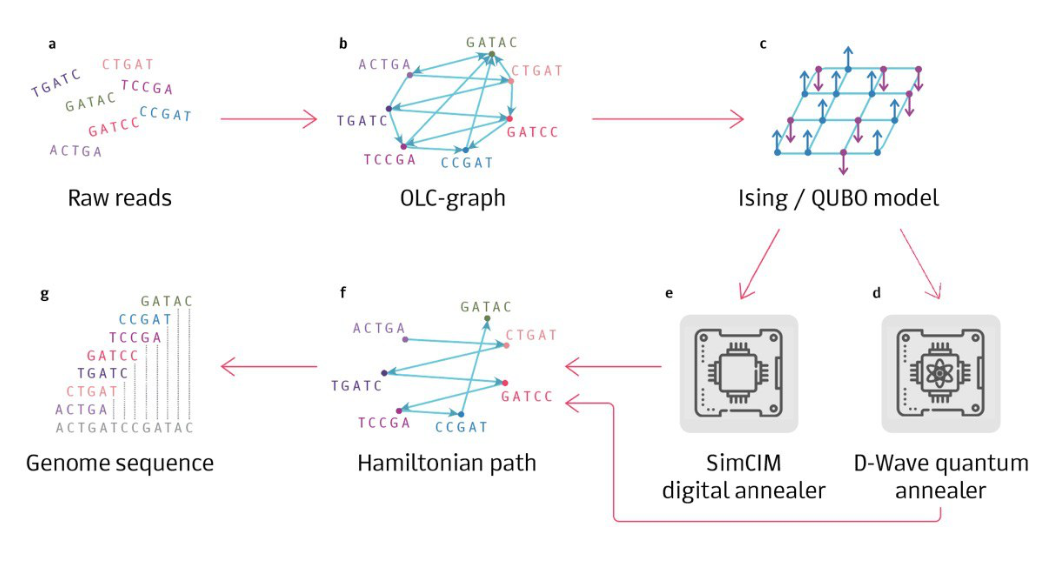
\includegraphics[scale=0.4]{de-novo-process.png}
	\centering
	\caption{Resolution diagram for the genome assembly using quantum annealing \cite{Boev2020}}
	\label{de-novo-process}
\end{figure}


\newparagraph{Numerical example}


Let us study a final numerical example based on \cite{Sarkar2020} that shows the whole process. Suppose we are given the following reads:

\begin{itemize}
	\item $r_0 = ATGGCGTGCA$
	\item $r_1 = GCGTGCAATG$
	\item $r_2 = TGCAATGGCG$
	\item $r_3 = AATGGCGTGC$
\end{itemize}

We may compute the overlap between the different reads. This results in the overlap graph from figure \ref{fig:overlap-graph}.

\begin{figure}[h]
	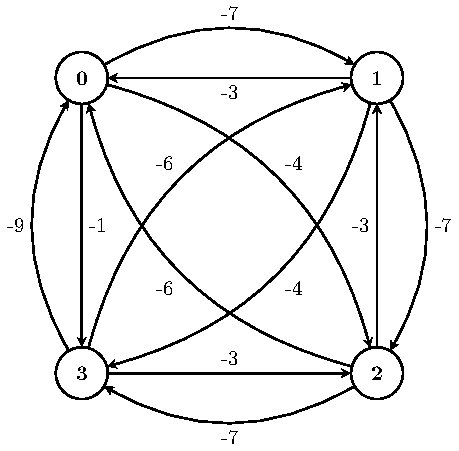
\includegraphics[scale=1.1]{graphs/salesman-example.pdf}
	\centering
	\caption{OLC graph}
	\label{fig:overlap-graph}
\end{figure}

Which is the same graph studied in the traveling salesman section, \ref{sec:salesman-example}. From the study done in that section, we know that there are six types of cycles in the graph. They are displayedin table \ref{tbl:salesman-cycles}. In figure \ref{fig:overlap-cycles}, we see how these types of cycles represent different ordinations of our DNA reads, as well as their overlaps and the total length of the resulting chain.

\begin{figure}[h]
	\makebox[\textwidth][c]{
		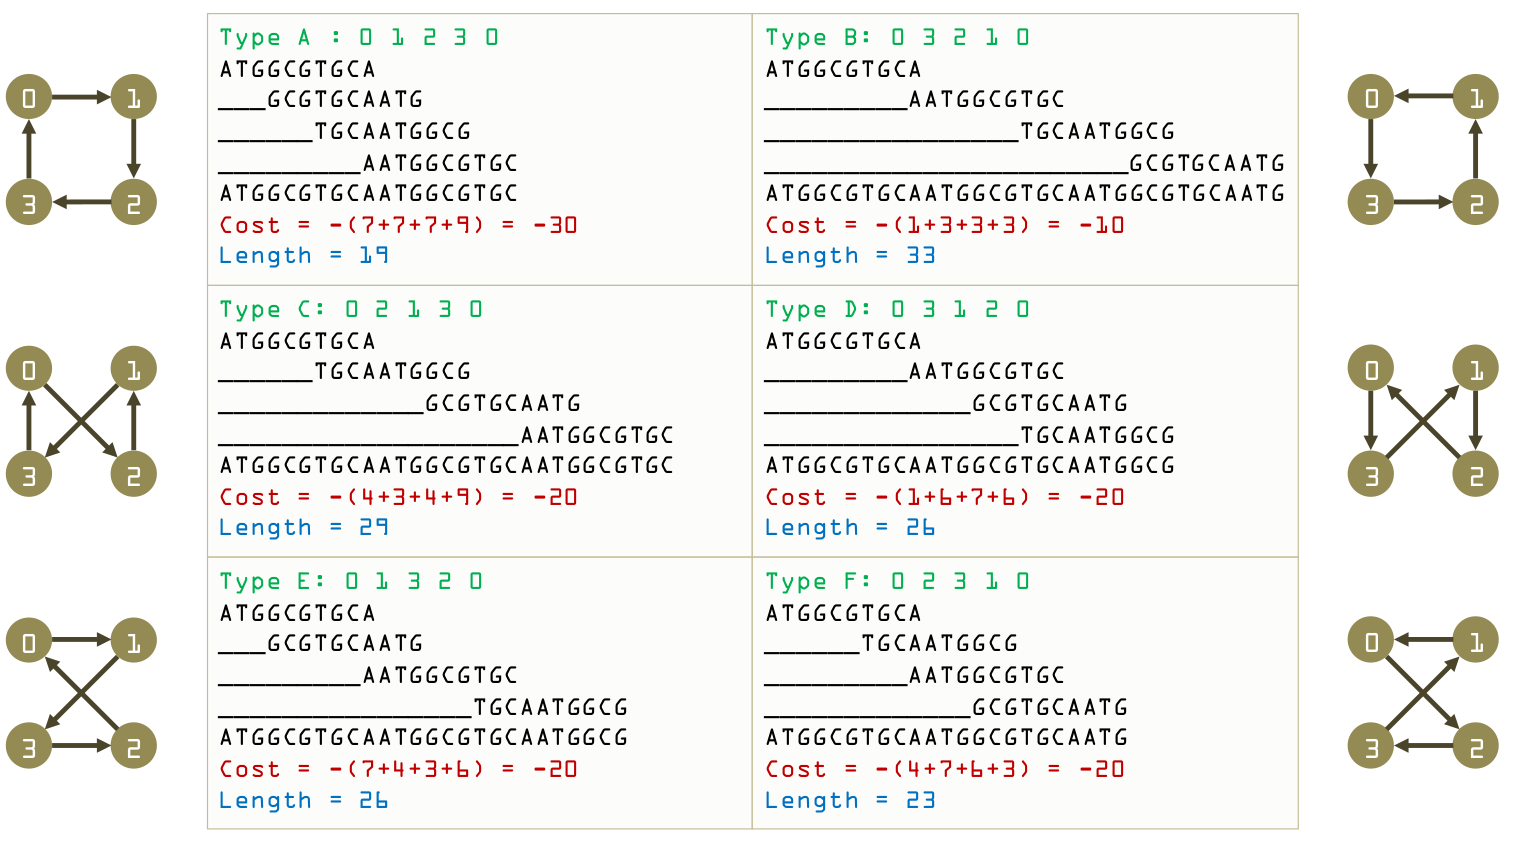
\includegraphics[scale=0.35]{overlap-cycles.png}
	}
	\centering
	\caption{Type of cycles and their corresponding overlap analysis \cite{Sarkar2020}}
	\label{fig:overlap-cycles}
\end{figure}

As we know, the type of Hamiltonian cycle that minimizes the cost is type A. This type translates into the shortest chain, with a total length of $19$. We can easily compute the resulting assembly by traversing the graph and weaving the reads together.


\section{Experimentation}
\label{sec:experimentation}


In this last section, we will explain the experiments reproduced using the D-Wave systems.


\subsection{How to reproduce the experiments}


In order to configure the samplers and submit jobs to D-Wave quantum annealers we used the \emph{D-Wave Ocean Software}, a suite of tools provided by D-Wave to use their quantum systems \cite{DWave-OceanDoc}. Using python and the provided packages we may connect to \emph{Leap}, a 'quantum' cloud service that provides access the quantum computers \cite{DWave-Leap}.

Leap provides a minute of free QPU time with the (free) developer plan. We may extend this time by obtaining either commercial or research access. This can be done by contacting the Leap team.

For the pourpose of this thesis I used the developer plan. In total, I submitted $104$ jobs to Leap, out of the allowed $106$. I consumed $59.064$ QPU seconds, as can bee seen in Leap's breakdown in figure \ref{fig:leap-breakdown}. The number of jobs and QPU time used in each system can be seen in table \ref{tab:leap-breakdown}.

\begin{table}[H]
	\centering
	\begin{tabular}{lrr}
		\textbf{System} & \textbf{Number of jobs} & \textbf{QPU time (s)} \\
		\hline
		D-Wave 2000Q	& 26	& 11.015	\\
		Advantage		& 77	& 46.681	\\
		Total			& 104	& 59.064                     
	\end{tabular}
	\caption{Leap usage summary breakdown between systems.}
	\label{tab:leap-breakdown}
\end{table}

Apart from Leap, in order to reproduce these experiments you will need to install tthe following Python packages, available thorugh \emph{pip}: \textbf{\emph{dimod}}, \textbf{\emph{neal}}, \textbf{\emph{minorminer}}, \textbf{\emph{dwave}} and \textbf{\emph{dwave\_networkx}}. The code I used for these experiments can be found in \cite{thesis-code}, which are inspired on \cite{Sarkar2020}.

\begin{figure}[H]
	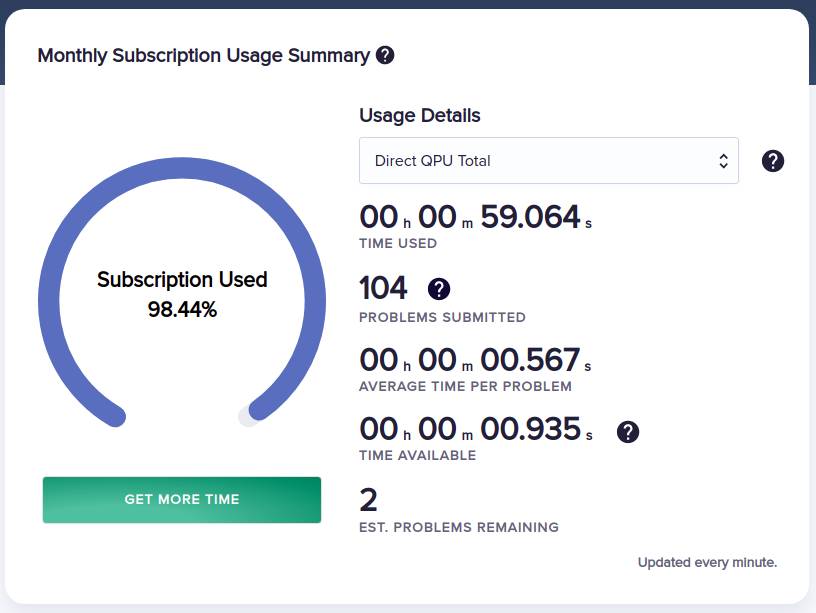
\includegraphics[scale=0.5]{experiments/leap-breakdown.png}
	\centering
	\caption{Leap monthly usage summary.}
	\label{fig:leap-breakdown}
\end{figure}


\subsection{Experiment 1: Data preparation and exact solving}


The first experiment aims to solve the previously discussed example using an exact solver provided by the Ocean's \emph{dimod} library \cite{Dimod}. The steps taken to transform the given reads to the QUBO matrix that Ocean's classes and functions use will be shared between the simulated annealer and the real quantum solvers. Therefore, the data preparation applied will be shared between experiments. The pseudocode of the experiment can be seen in the following snippet.

\begin{algorithm}
	\caption*{\textbf{Experiment 1}}
	
	Data preparation:
	\begin{itemize}
		\item Compute the distance between every two reads, creating an adjacency matrix.
		\item Transform the TSP adjancency matrix into a QUBO $Q$ matrix, as explained in section \ref{sec:tsp-qubo}.
		\item Transform the QUBO matrix into an adjacency dictionary.
	\end{itemize}

	Solving:
	\begin{itemize}
		\item Initiaize a sampler: \textbf{\emph{dimod.ExactSolver}}.
		\item Solve the prepared QUBO model using the selected solver.
	\end{itemize}
	
	Present the results.
\end{algorithm}

As we already know, using quantum annealing does not guarantee that we will obtain the optimal solution for a given cost function. In order to overcome this problem we use multi-sampling: running the experiment multiple times and and look at the best obtained solutions. Ocean already implements different types of \emph{samplers} to facilitate this task \cite{DWave-OceanDoc-Samplers}. In this first experiment we use an \emph{ExactSolver}, which simply check every possible solution. Although time-costly, this method will let us know if our data manipulation before solving the experiment is correct, and how the solutions landscape looks like.

The third step in data preparation is a formatting step. Ocean requires the QUBO and Ising models to be in an adjacency dictionary instead of a matrix. Let us look at an example of this transformation in order to better understand it. Consider a 2-reads, the associated TSP will have $2^2 = 4$ nodes: $n0t0$, $n0t1$, $n1t0$ and $n1t1$. Suppose the following (inconsistency) matrix is the associated $Q$ matrix:

$$
Q = 
\left(
\begin{array}{cccc}
	1 & 2 & 3 & 4 \\
	5 & 6 & 7 & 8 \\
	9 & 10 & 11 & 12 \\
	13 & 14 & 15 & 16 
\end{array}
\right)
$$

Then, it will be transformed into the dictionary, with $11$ missing entries: 

\begin{minted}[bgcolor=bg]{python}
quboDict: {
	('n0t0', 'n0t0'): 1,
	('n0t0', 'n0t1'): 2,
	('n0t0', 'n1t0'): 3,
	('n0t0', 'n1t1'): 4,
	...
	('n1t1', 'n1t1'): 16,
}
\end{minted}

In particular, this experiment is applied to the already studied example with the following four reads:

\begin{itemize}
	\item $r_0 = ATGGCGTGCA$
	\item $r_1 = GCGTGCAATG$
	\item $r_2 = TGCAATGGCG$
	\item $r_3 = AATGGCGTGC$
\end{itemize}

The pair-wise distances are computed, providing a direct measure of much two reads overlap. Then, these values are normalized for easier use. The resulting normalized TSP matrix is transformed into a QUBO matrix using $1.6$ as multi-location and repetition penalties, and $-1.6$ for self-bias, as done in \cite{Sarkar2020}. Finally, we initialize an \emph{ExactSolver} and use it to sample every possible solution.

After the execution is completed, we find the lowest energy in the obtained solutions and print every solution with that energy:

\begin{minted}[bgcolor=bg]{python}
{'n0t0': 0, 'n0t1': 0, 'n0t2': 1, 'n0t3': 0,
 'n1t0': 0, 'n1t1': 0, 'n1t2': 0, 'n1t3': 1,
 'n2t0': 1, 'n2t1': 0, 'n2t2': 0, 'n2t3': 0,
 'n3t0': 0, 'n3t1': 1, 'n3t2': 0, 'n3t3': 0} --> -7.9811

{'n0t0': 0, 'n0t1': 1, 'n0t2': 0, 'n0t3': 0,
 'n1t0': 0, 'n1t1': 0, 'n1t2': 1, 'n1t3': 0, 
 'n2t0': 0, 'n2t1': 0, 'n2t2': 0, 'n2t3': 1, 
 'n3t0': 1, 'n3t1': 0, 'n3t2': 0, 'n3t3': 0} --> -7.9811

{'n0t0': 1, 'n0t1': 0, 'n0t2': 0, 'n0t3': 0,
 'n1t0': 0, 'n1t1': 1, 'n1t2': 0, 'n1t3': 0, 
 'n2t0': 0, 'n2t1': 0, 'n2t2': 1, 'n2t3': 0, 
 'n3t0': 0, 'n3t1': 0, 'n3t2': 0, 'n3t3': 1} --> -7.9811

{'n0t0': 0, 'n0t1': 0, 'n0t2': 0, 'n0t3': 1,
 'n1t0': 1, 'n1t1': 0, 'n1t2': 0, 'n1t3': 0,
 'n2t0': 0, 'n2t1': 1, 'n2t2': 0, 'n2t3': 0,
 'n3t0': 0, 'n3t1': 0, 'n3t2': 1, 'n3t3': 0} --> -7.9811
\end{minted}

As expected, these are the four minimums of the cost functions, representing the four ways of describing a type A loop in the used codification.

Finally, let us plot the landscape of solutions for the given reads. We sort the solutions by increasing energy and simply plot their energy, as seen in figure \ref{fig:exp1-landscape}.

\begin{figure}[H]
	\makebox[\textwidth][c]{
		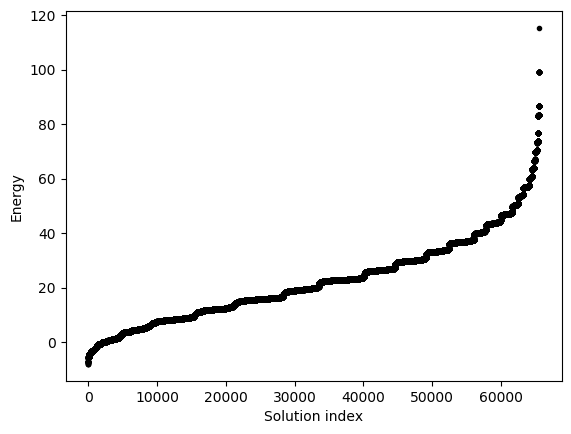
\includegraphics[scale=0.7]{experiments/experiment1.png}
	}
	\centering
	\caption{Landscape of solutions}
	\label{fig:exp1-landscape}
\end{figure}


\subsection{Experiment 2: Simulated Quantum Annealing}

For our second experiment, we aim to solve our example using Simulated Annealing. Although \emph{dimod} provides a simulated annealing sampler, we use for our final experiments the  \emph{SimulatedAnnealingSampler} from \emph{Ocean}'s \emph{Neal} package as it yields more distributed results and has far better computing time. The same experiment was reproduced $10$ times using both samplers in my machine. Dimod's sampler run in a mean time of $11.76$ seconds while \emph{Neal}'s run in a mean time of $0.0610$ seconds.

The pseudo-code does not change much from the first experiment to the second one, we simply change the annealer:

\begin{algorithm}
	\caption*{\textbf{Experiment 2}}
	
	Data preparation:
	\begin{itemize}
		\item Compute the distance between every two reads, creating an adjacency matrix.
		\item Transform the TSP adjancency matrix into a QUBO $Q$ matrix, as explained in section \ref{sec:tsp-qubo}.
		\item Transform the QUBO matrix into an adjacency dictionary.
	\end{itemize}
	
	Solving:
	\begin{itemize}
		\item Initiaize a sampler: \textbf{\emph{neal.SimulatedAnnealingSampler}}.
		\item \textbf{Sample from} the prepared QUBO model using the selected \textbf{sampler}.
	\end{itemize}
	
	Present the obtained samples.
\end{algorithm}

It is worth mentioning that we do not \emph{solve} the QUBO model in these experiments, we \emph{sample} different results using simulated annealing.

Since \emph{Neal}'s sampler is quite efficient we were able to execute experiments with up to $10.000$ repetitions of the experiment, also called \emph{sample reads} or simply \emph{reads}. We developed an automated and scalable way to check whether a given cycle returned by the annealer was valid, and to recover its associated type. Using these tools we can easily check the number of occurrences each type of cycle appeared in the obtained sample reads. These results are presented, along with the associated energy to each result, in table \ref{tab:exp2} and figure \ref{fig:exp2-occ}. See figure \ref{fig:overlap-cycles} to recall the cycle types and cost computing.

\begin{table}[H]
	\centering
	\begin{tabular}{lrr}
		\textbf{Cycle type} & \textbf{Occurences} & \textbf{Energy} \\
		\hline
		Type A	& 3722	& -7.9811	\\
		Type C	& 1474	& -7.4541	\\
		Type D	& 1469	& -7.4541	\\
		Type F	& 1458	& -7.4541	\\
		Type E	& 1431	& -7.4541	\\
		Type B	& 446	& -6.927                             
	\end{tabular}
	\caption{Results of experiment 2}
	\label{tab:exp2}
\end{table}

\begin{figure}[H]
	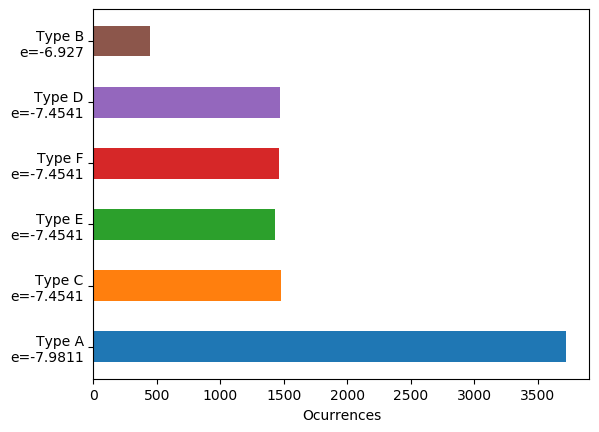
\includegraphics[scale=0.8]{experiments/experiment2.png}
	\centering
	\caption{Ocurrences of each type in a $10.000$ reads experiment using Simulated Annealing}
	\label{fig:exp2-occ}
\end{figure}

We can appreciate in figure \ref{fig:exp2-occ} that the best type of cycle agglomerates most of the samples, $37.22\%$. In the second place, the four types of cycles that have the exact same energy also have almost exactly the same number of samples. This matches our quantum annealing theory: the physical system has an equal probability of ending in eigenstates with equal eigenenergies.

It is worth mentioning that there was not a single sample that encoded an invalid cycle. This means that the penalties values used for the experiment ($1.6$ for multi-location and repetition, and $-1.6$ for self-bias) are working to prevent invalid cycles.

Now that we are familiar with the type of results and codifications we may find, let us jump to the quantum realm by using the D-Wave's Quantum Computer Systems.


\subsection{Experiment 3: Quantum Annealing using D-Wave}


For our third experiment, we aim to solve our example using D-Wave's quantum annealers. For this purpose, we need to add some extra steps to our data processing. Section \ref{sec:embeddings} explained how not every graph can be directly mapped to the existing Chimera / Pegasus topologies that D-Wave systems use, and how we can overcome this problem by embedding our problems graphs into these topologies. The extra steps in our data processing are related to these embeddings: we will need to embed our graph into the fixed topology that will be used. Then, after the anneal takes place, we will translate the solutions from the embedded graph. Ocean provides a set of utilities to deal with these embeddings \cite{DWave-OceanDoc-Embedding}.

Additionally, we will need to connect to Leap to send our jobs to the quantum annealers using a \emph{client}. First, a configuration file is created, which includes your API key and some extra configuration details:

\begin{minted}[bgcolor=bg]{bash}
[ocete]
solver = {"qpu": true}
token = DEV-<api key goes here>
endpoint = https://cloud.dwavesys.com/sapi
\end{minted}

In our code we initialize a \emph{client} and a \emph{solver} using the configuration file. These are objects that encapsulate the connection functionality and solving problems in the associated machine respectively. We also initialize a sampler as we did before, but this time a production sampler is used: a \emph{DWaveSampler} that also needs our configuration file. The pseudo-code for this experiment can be found below. Each new step will be explained in detail below.

\begin{algorithm}
	\caption*{\textbf{Experiment 3}}
	
	Initialization:
	\begin{itemize}
		\item Initiaize a sampler: \textbf{\emph{system.samplers.DWaveSampler}}.
		\item \textbf{Initialize a client and obtain an associated solver}.
	\end{itemize}
	
	Data preparation:
	\begin{itemize}
		\item Compute the distance between every two reads, creating an adjacency matrix.
		\item Transform the TSP adjacency matrix into a QUBO $Q$ matrix, as explained in section \ref{sec:tsp-qubo}.
		\item Transform the QUBO matrix into an adjacency dictionary.
		\item \textbf{Find an embedding from our graph to the selected machine's topology (either Chimera or Pegasus)}.
		\item \textbf{Use the previous embedding to create a new QUBO model equivalent for the embedded graph}.
	\end{itemize}
	
	Solving:
	\begin{itemize}
		\item Use the solver to send a job to the client. This job samples from the prepared QUBO model multiple times.
	\end{itemize}
	
	Format the results:
	\begin{itemize}
		\item \textbf{Use the computed embedding to translate our answers}.
	\end{itemize}
\end{algorithm}

The first thing to be noticed is that the initialization now needs to be done before the data preparation. This is because, in order to find the embedding, we need to know which exact topology the quantum system will have. This information is provided through the \emph{solver}, previously initialized. The initialization step is as simple as follows:

\begin{minted}[bgcolor=bg]{python}
import dwave

# Create the solver (connecting to D-Wave) and the Sampler
config_file='../dwave.conf'
client = cloud.Client.from_config(config_file, profile='ocete')
solver = client.get_solver()
dwsampler = system.samplers.DWaveSampler(config_file=config_file)
\end{minted}

Suppose $Q$ already holds our computed QUBO model. We can compute an embedding and obtained the new associated model as follows:

\begin{minted}[bgcolor=bg]{python}
adjacency_dict = embedding.utils.edgelist_to_adjacency(solver.edges)
embedding = minorminer.find_embedding(Q, solver.edges)
Q_embedded = embed_qubo(Q, embedding, adjacency_dict)
\end{minted}

By using the same configuration file, the sampler already knows what machine it is associated to. We will sample from it, with the same syntax as in the second experiment:

\begin{minted}[bgcolor=bg]{python}
response = dwsampler.sample_qubo(Q_embedded, num_reads=num_reads)
\end{minted}

Where $num\_reads$ is a parameter that sets the number of samples to be read. However, these solutions are associated to the $Q\_embedded$, not to our original $Q$ model. We need to translate the responses to understand them:

\begin{minted}[bgcolor=bg]{python}
bqm = dimod.BinaryQuadraticModel.from_qubo(Q)
unembedded_response = embedding.unembed_sampleset(response, embedding, bqm)
\end{minted}

For this experiment, the D-Wave 2000Q was used (see section \ref{sec:d-wave-systems} to see its characteristics), since it was the default solver. After running the experiment with the same parameters as the simulated annealing experiment ($10.000$ reads and $(-1.6; 1.6; 1.6)$ for the QUBO parameters), we obtained that more than $90\%$ of the samples were invalid, a huge difference with the astonishing $0\%$ obtained in the second experiment.

My initial hypothesis was that the QUBO parameters were well adjusted for SA but not for QA, and thus allowed further tunning. After many attempts with different parameters values, this hypothesis was discarded. The only other set of parameters worth presenting is $(-1.5; 1.5; 1.5)$. These results are presented in table \ref{tab:exp3}.

\begin{table}[H]
	\centering
	\begin{tabular}{lrrr}
		\textbf{Cycle type} & \textbf{Occurences (param=1.5)} & \textbf{Occurences (param=1.6)} & \textbf{Energy} \\
		\hline
		Type A	& 131	& 50	& -7.9811	\\
		Type C	& 124	& 46	& -7.4541	\\
		Type D	& 40	& 91	& -7.4541	\\
		Type F	& 55	& 117	& -7.4541	\\
		Type E	& 112	& 118	& -7.4541	\\
		Type B	& 99	& 64	& -7.4541	\\    
		Invalid & 9221	& 9194	& $>$ -5.6433                         
	\end{tabular}
	\caption{Results of experiment 3, $10.000$ reads using the quantum annealer.}
	\label{tab:exp3}
\end{table}

In figures \ref{fig:exp3-occ1} and \ref{fig:exp3-occ2} we see a comparison of the distribution between the different type of cycles in both experiments. We cannot see a distribution as we did in \ref{fig:exp2-occ}, potentially due to the low numbers of reads that actually represent a valid cycle. In fact, such distribution between the cycle types is not needed: a single sample with the lowest energy solution will completely solve our genome assembly problem.

\begin{figure}[H]
	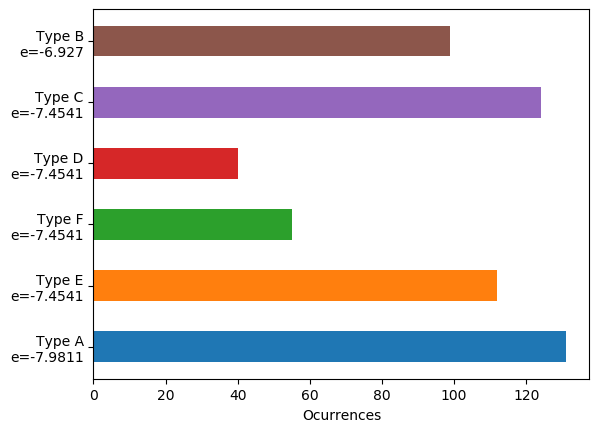
\includegraphics[scale=0.75]{experiments/experiment3 (1.5).png}
	\centering
	\caption{Ocurrences of each cycle type in a $10.000$ reads experiment using Quantum Annealing, filtering out invalid cycles, with QUBO parameters $(-1.5; 1.5; 1.5)$}
	\label{fig:exp3-occ1}
\end{figure}

\begin{figure}[H]
	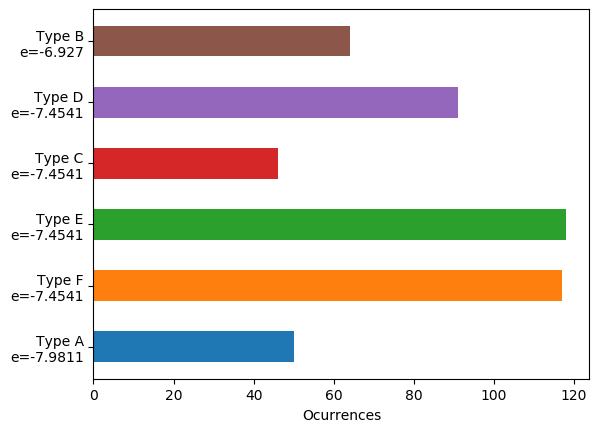
\includegraphics[scale=0.75]{experiments/experiment3 (1.6).png}
	\centering
	\caption{Ocurrences of each cycle type in a $10.000$ reads experiment using Quantum Annealing, filtering out invalid cycles, with QUBO parameters $(-1.6; 1.6; 1.6)$}
	\label{fig:exp3-occ2}
\end{figure}

With these results in mind, is it possible that we are sampling completely random solutions? In a 4-reads problem, we obtain a 16 binary variables QUBO model. That means there are up to $2^{16}$ possible solutions using our encoding, even more after we embed it in the Chimera topology. If we were to randomly sample from that solution space, we will never get almost $10\%$ of samples from a subset of $24$ solutions that represent our $6$ valid cycles. So we do know that the quantum system is working, just not as good as expected.

We have not found a clear improvement precision-wise in our small example, although QA does solve the problem. What about time-wise? In figure \ref{fig:exp3-time} we see the time breakdown provided by Leap after our last experiment. We can see a total QPU sampling time of $2.389$ seconds, while if we repeat the experiment with the same parameters using SA we obtain a mean of $2.525$ sampling seconds, over $10$ experiment repetitions. Keeping in mind that our QA time data comes from a single execution and the small difference between both time measures, we cannot conclude that either approach has any time advantage in such small problems.

However, does QA actually scales better than SA with the problem size? In the next experiment, we will study the Pegasus topology to understand what is the maximum problem size that can be tackled using the Advantage system. Finally, the last couple of experiments will try to answer the scalability comparison inquiry.

\begin{figure}[h]
	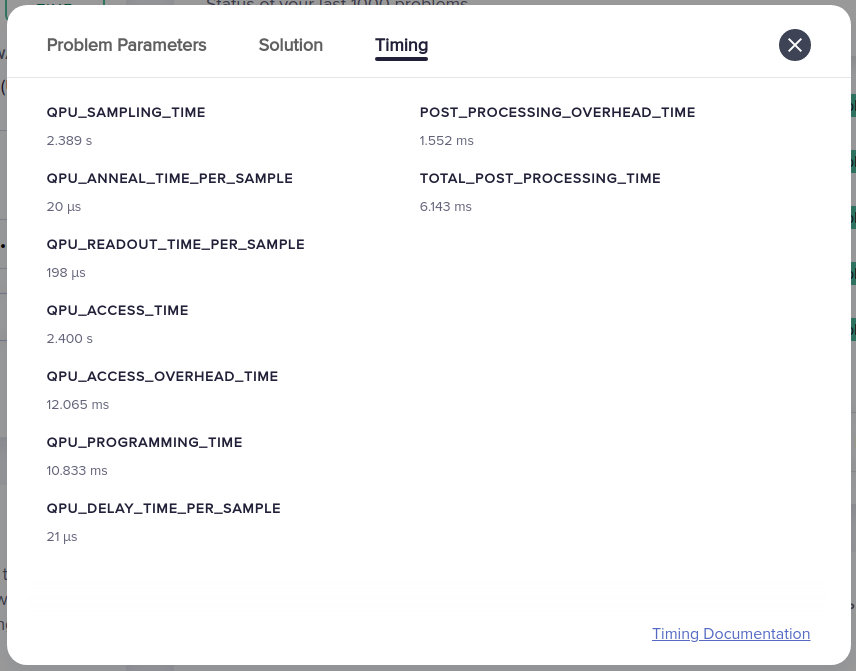
\includegraphics[scale=0.5]{experiments/exp3-time.png}
	\centering
	\caption{Time breakdown provided by Leap after the last experiment.}
	\label{fig:exp3-time}
\end{figure}


\subsection{Displaying chimera embeddings}


Let us plot some logical embeddings using the D-Wave 2000Q system, with relies on a Chimera graph. In figure \ref{fig:exp2_4reads} we see the embedding of a 4-nodes complete graph into the Chimera topology. The grey nodes represent unused nodes while nodes with the same color represent a single logical qubit mapped into multiple physical qubits.

\begin{figure}[h]
	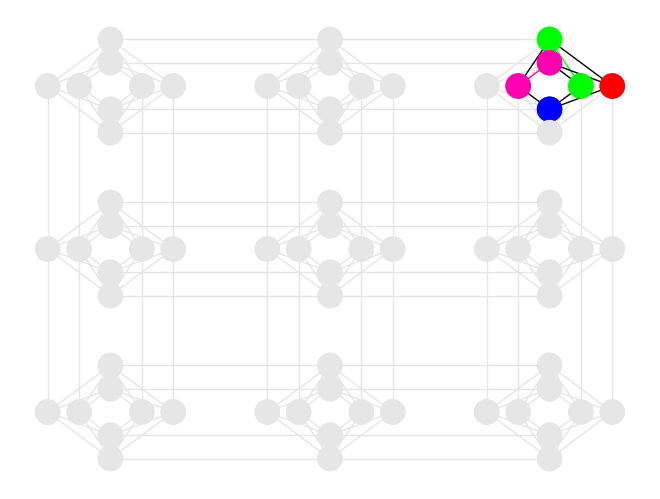
\includegraphics[scale=0.6]{experiments/exp2_4reads.png}
	\centering
	\caption{Embedding of a 4-nodes complete graph into a Chimera topology.}
	\label{fig:exp2_4reads}
\end{figure}

The last embedding had a \emph{maximum chain length} of $2$. That is, the longest chain in a logical qubit is 2 physical qubits. This is a critical parameter to be minimized in embeddings: the longer the qubit chain is, the more probable it is for the qubits in a logical qubit to be desynchronized and end up in different states. Thus, the more difficult it is for the system to stay in the ground state.

In figure \ref{fig:exp2_13reads} we see an embedding of a 13-nodes complete graph into a Chimera topology. In this case, the maximum chain length is $5$, obtained by both the dark blue, purple, red, dark green, lime, and cyan logical qubits. In the rest of the experiments, I looked at the maximum chain length obtained in the pegasus embeddings, obtained lengths up to $15$ qubits. Since I did not have the time to study this characteristic in-depth, it will be a future line of work.

\begin{figure}[h]
	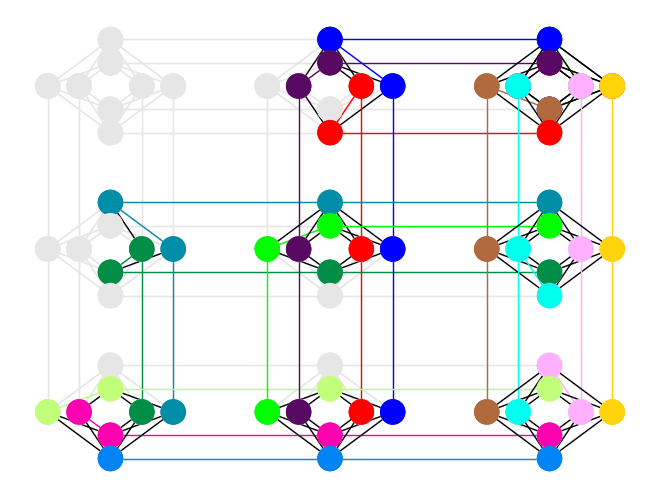
\includegraphics[scale=0.6]{experiments/exp2_13reads.png}
	\centering
	\caption{Embedding of a complete 13-nodes complete graph into a Chimera topology.}
	\label{fig:exp2_13reads}
\end{figure}

Recall that in every 16-nodes chimera cell, every node in the vertical axis is connected to every node in the horizontal axis, and to no other node from the vertical axis. For example, take the blue logical qubit, represented by 3 nodes at the very bottom in figure \ref{fig:exp2_13reads}. In the first cell, it connects with lime, pink, dark green, and cyan. In the second cell, it connects with light green, purple, red, and dark blue. In the third cell, it connects to brown, light blue, pink, and yellow. That makes a total of 12 connections, as expected since the embedded started with a complete 13-nodes graph.


\FloatBarrier
\subsection{Experiment 4: D-Wave's Advantage limits}


For our fourth experiment, we aim to test the limits of the Advantage architecture for our problem. That is, given a number of DNA reads, we will compute the associated QUBO problem and try to embed the obtained graph into the Advantage architecture. We will test these embeddings against a Pegasus 16 ($P_{16}$) topology since that is the one supported by the Advantage system.

In fact, given a set of $n$ reads, this is simply finding if a $n^2$-nodes complete graph ($K_{n^2}$) can be embedded into a $P_{16}$. The reads themselves are not relevant for the embedding. However, I have developed an automated way of creating fake tests, originally for a general-purpose, but it can also be used here.

This automated test production works as follows: Given a number of reads, the size of each chain (default value $150$), and the required overlap between adjacent chains (default value $50$), it randomly creates the original DNA chain, and then chop it using the given parameters. This makes sure that adjacent reads have enough overlap so it is basically impossible for two random reads to overlap more than $50$ bps.

Using these random tests we created graphs of an increasing number of reads until we were unable to find an embedding from $K_{n^2}$ to $P_{16}$. The results of the experiment can be seen in table \ref{tab:exp4}. We can see that a valid embedding was found to problem size up to 14 reads ($K_{196}$ associated graph). The embedding time, as well as the test generation time, are also displayed. I decided to display both since, as time grew larger and larger, I was not sure whether the test generation was adding too much of an overload.

\begin{table}[H]
	\centering
	\makebox[\textwidth][c]{
		\begin{tabular}{ccccc}
			\textbf{Number of reads} & \textbf{Nodes in graph} & \textbf{Test generation time} & \textbf{Embedding time} & \textbf{Total time} \\
			\hline
			2   & 4   &  0.000157   &  0.081310   &  0.081708 \\
			3   & 9   &  0.000216   &  0.108525   &  0.109205 \\
			4   & 16   &  0.000269   &  0.194807   &  0.196045 \\
			5   & 25   &  0.000335   &  0.377673   &  0.379814 \\
			6   & 36   &  0.000392   &  1.147603   &  1.154559 \\
			7   & 49   &  0.000433   &  3.514801   &  3.523473 \\
			8   & 64   &  0.000497   &  11.876785   &  11.888235 \\
			9   & 81   &  0.000558   &  19.226392   &  19.244367 \\
			10   & 100   &  0.000610   &  43.457666   &  43.477268 \\
			11   & 121   &  0.000676   &  62.499896   &  62.528545 \\
			12   & 144   &  0.000724   &  89.277396   &  89.313831 \\
			13   & 169   &  0.000812   &  63.782066   &  63.827706 \\
			14   & 196   &  0.000840   &  152.262340   &  152.316223
		\end{tabular}
	}
	\caption{Results of experiment 4}
	\label{tab:exp4}
\end{table}

It is worth noting that the algorithm used to find the embeddings does not guarantee to find a valid one if it exists. I tried to run the algorithm $50$ times with $15$ reads and could not find a valid embedding.

The reader might have already noticed that the embeddings are quite time-consuming. In fact, this is an NP problem itself and time will grow exponentially on input size. However, keep in mind that this embedding does not depend on the reads. Once a single embedding from a $K_{196}$ to a $P_{16}$ has been pre-computed it can be used -or further optimized- for different problems.

Now that we know the maximum number of reads that the Advantage system may tackle, let us put it to the test with 'big' input problems in the next experiment.


\subsection{Experiment 5: Scalability comparison between Simulated Annealing and Quantum Annealing}


In our fifth experiment, we put the D-Wave's quantum annealers to the test with bigger input problems and study how they behave compared with the simulated annealing experiments. We will start with a $3$ reads and then progressively increase this value, creating tests of this size and trying to solve them using both the simulated annealer and the Advantage system.

For each fixed number of reads, we will sample $10.000$ times using the annealers, with the same set of parameters used for the previous experiments. The number of valid solutions (i.e. valid cycles) will be displayed, along with the number of cycles that reached the real solution, which we know in advance since we created the test.

We will also display the energy of the best sample obtained, along with the difference between the real solution energy and the best sample obtained, which I called \emph{energy delta}. Finally, we will also display the sampling time, not including the time it took to create the test nor to prepare the data.

The results of this experiment using the simulated annealer can be seen in table \ref{tab:exp5_1}. 

\begin{table}[H]
	\centering
	\makebox[\textwidth][c]{
		\begin{tabular}{cccccc}
			\textbf{N. reads} & \textbf{Valid cycles} & \textbf{Times sol. reached} & \textbf{Energy delta} & \textbf{Solution energy} & \textbf{Sampling time} \\
			\hline
			3	& 10000		& 9564			& 0				& -6.214214		& 1.881374 \\
			4	& 10000		& 6852			& 0				& -8.131935		& 2.178147 \\
			5	& 10000		& 3427			& 0				& -9.999001		& 3.487972 \\
			6	& 10000		& 1308			& 0				& -11.834192	& 5.121054 \\
			7	& 10000		& 351			& 0				& -13.656181	& 7.057235 \\
			8	& 10000		& 108			& 0				& -15.443562	& 9.680610 \\
			9	& 10000		& 21			& 0				& -17.232667	& 12.797996 \\
			10	& 10000		& 3				& 0				& -18.995278	& 16.080461 \\
			11	& 10000		& 0				& 0.625356		& -20.764680	& 20.118828 \\
			12	& 10000		& 0				& 0.601820		& -22.510011	& 25.351562 \\
			13	& 10000		& 0				& 0.570361		& -24.256735	& 30.612547 \\
			14	& 10000		& 0				& 1.378872		& -26.005003	& 34.897780
		\end{tabular}
	}
	\caption{Results of experiment 5, $10.000$ reads using the simulated annealer.}
	\label{tab:exp5_1}
\end{table}

We stopped at 15 reads since that is the maximum value that will be able to compare with using the quantum annealer. In the experiment results, we see how the number of valid cycles out of $10.000$, which turns out to be every single cycle up to 14 reads. However, the number of samples that reached the best solution go down from $95\%$ to ground cero from $11$ reads onward. Although we do not obtain the real solution, how close are these samples to it? 

The columns related to the energy of the solutions try to answer this question. We may see how the solution's energy goes down to around $-26$, which is totally normal: the more reads in our graph, the higher the number of reads overlap, and the lower is the resulting solution energy. As soon as we cannot find the solution, the energy delta starts to increase, going up to around $1.37$. This means the energy of the best sample is quite close to the actual value. Is this enough?

When we tackle a classic TSP, a near-optimal solution is a really valid and useful solution. We do not necessarily need the actual minimum. However, although a valid cycle with low energy represents a valid way of sorting and sewing the genome reads, it does not provide the real genome the reads came originally from. It has some value since it could be further tuned to obtain the solution, but it does not solve our problem.

Lastly, the sampling time seems to grow linearly with the number of reads. However, using this simple simulated annealer for a real case with up to 3 Mbps would be simply impossible.

For the second part of this experiment, I run the same experiment but using the quantum annealer. Some extra steps come with it, like computing the embedding and connecting to Leap, but they have all been explained in previous experiments. We again sample $10.000$ times a maintain the same values for the annealing schedule self-bias, multi-location, and repetition parameters. The results of this experiment can be seen in table \ref{tab:exp5_2}.

\begin{table}[H]
	\centering
	\makebox[\textwidth][c]{
		\begin{tabular}{cccccc}
			\textbf{N. reads} & \textbf{Valid cycles} & \textbf{Times sol. reached} & \textbf{Energy delta} & \textbf{Solution energy} & \textbf{Sampling QPU time} \\
			\hline
			3	& 4574		& 3295		& 0				& -6.214214		& 1.035 \\
			4	& 683		& 156		& 0				& -8.131935		& 0.962 \\
			5	& 88		& 6			& 0				& -9.999900		& 1.272 \\
			6	& 2			& 0			& -1.322536		& -11.834014	& 1.272 \\
			7	& 1			& 0			& -1.647457		& -13.671186	& 1.206 \\
			8	& 0			& 0			& -3.867139		& -15.444996	& 1.339 \\
			9	& 0			& 0			& -36.592409	& -17.227226	& 1.570 \\
			10	& 0			& 0			& -50.03568		& -18.468571	& 1.276
		\end{tabular}
	}
	\caption{Results of experiment 5, $10.000$ reads using the quantum annealer.}
	\label{tab:exp5_2}
\end{table}

The first thing we may notice is that the experiment did not reach 14 reads. That is because I manually stopped it before it finished. The available QPU time was quite tight at the moment, and seeing the results of the experiment with a number of reads up to $10$ showed that we were not going to learn anything new by letting the experiment finished and wasting our remaining QPU time.

Back to the results, we can appreciate the number of valid cycles rapidly goes down to $0$, and even quicker the number of reads that reached the solution. At 4 reads we see similar results to what we saw in experiment 3: around $700$ valid cycles and $150$ times the real solution (type A cycle in the third experiment) was reached. Although we have developed this experiment in different machines, D-Wave 2000Q and Advantage, keep in mind that the improvements from one generation to another are size-related: we may tackle bigger (and thus harder) problems by using the Advantage system. It does not mean that its computation is somehow better.

Not only the responses are not valid, but they are also quite far from the solution. We can see that in how the delta grows hugely as we increase the number of reads. Leap provides a graph for each submitted experiment displaying the samples' distribution. In figures \ref{fig:exp5_1} and \ref{fig:exp5_2} we see this distribution for $4$ and $10$ reads respectively. 

\begin{figure}[H]
	\includegraphics[scale=0.5]{experiments/exp5_1.png}
	\centering
	\caption{$10.000$ samples' distribuition for $4$ reads using the quantum annealer.}
	\label{fig:exp5_1}
\end{figure}

\begin{figure}[H]
	\includegraphics[scale=0.5]{experiments/exp5_2.png}
	\centering
	\caption{$10.000$ samples' distribuition for $10$ reads using the quantum annealer.}
	\label{fig:exp5_2}
\end{figure}

We can see how in the $4$ reads experiment, most of the samples group around $0$ energy, and only a very few are close to the solution, which is actually reached in this execution. However, in the $10$ reads experiment, most of the samples are gathered around $100/150$ energy, these solutions are not only invalid but really far from being so.

Lastly, let us comment on the QPU sampling time. This value is provided directly by Leap. From our code, we cannot separate the connection overload and other computations from the actual QPU sampling time. We may appreciate how time does not grow with the input. This is because the time it takes for the annealer to converge is fixed by the annealing schedule.

In conclusion, these results are astonishingly awful. The simulated annealing sampler not only provides closer samples to the solution, but in every seen case it reaches valid samples. My current hypothesis is that either the annealing schedule is not optimal, or that the values of the parameters can be improved for our specific problem. In our last experiment, I will spend all our remaining QPU time checking these two hypotheses.


\subsection{Experiment 6: Advantage tunning}


For our last experiment, we aim to test our previous hypothesis and try to solve a $10$ reads problem using the Advantage system. In the first set of iterations, I tried to increase the multi-location and repetition penalties in order to increase the number of valid cycles sampled. For this experiment, a single test with $10$ reads was created. Its solution energy was  $-18.994150$. The results of the experiment can be found in table \ref{tab:exp6_1}, where the mentioned parameters are \emph{(self-bias, multi-location, repetition)}.

\begin{table}[H]
	\centering
	\makebox[\textwidth][c]{
		\begin{tabular}{ccccc}
			\textbf{Parameters} & \textbf{Valid cycles} & \textbf{Times sol. reached} & \textbf{Energy delta} & \textbf{Sampling QPU time} \\
			\hline
			(-1.6, 1.6, 1.6)	& 0		& 0			& -76.344431	&	1.500 \\
			(-3, 3, 3)			& 0		& 0			& -87.263801	&	1.624 \\
			(-5, 5, 5)			& 0		& 0			& -83.657639	&	1.272 \\
			(-10, 10, 10)		& 0		& 0			& -258.290739	&	1.248 \\
			(-20, 20, 20)		& 0		& 0			& -357.917063	&	1.311 \\
			(-50, 50, 50)		& 0		& 0			& -1017.605383 	&	1.441 \\
			(-100, 100, 100)	& 0		& 0			& -1418.541757 	&	1.261
		\end{tabular}
	}
	\caption{Results of experiment 6, $10.000$ reads using the quantum annealer for different parameters configurations.}
	\label{tab:exp6_1}
\end{table}

As we can see in the table, we did not find a single valid cycle in these iterations. The energy delta naturally increases as we increase the parameter values: every single penalty is greater penalized. However, the energy delta barely increases until our parameters get a value of $10$. This could show how the responses for \emph{parameters} $= (-5, 5, 5)$ incurred in a lower number of penalties. In figure \ref{fig:exp6_1} we find the samples distribution for \emph{parameters} $= (-5, 5, 5)$. The overall energy is much higher than what we saw for \emph{parameters} $= (-1.6, 1.6, 1.6)$ in figure \ref{fig:exp5_2}, which occurs due to the higher penalty. This experiment concludes that either we have not been able to find the correct values for the parameters, or the values of the parameters are not the problem.

\begin{figure}[H]
	\includegraphics[scale=0.5]{experiments/exp6_1.png}
	\centering
	\caption{$10.000$ samples distribuition for \emph{parameters} $= (-5, 5, 5)$.}
	\label{fig:exp6_1}
\end{figure}

Finally, we try changing the annealing schedule. There are two possible parameters that we may modify in this sense: the \emph{annealing time} -time let for the annealer to converge-, or the \emph{annealing schedule} -which modifies the annealing functions as defined in figure \ref{fig:dwave-annealing-functions}. Since my initial hypothesis was that the annealer did not have enough time to find good solutions, let us focussed on the former for our last experiment.

The anneal time is meassured in microseconds, with a default value of $20$. Although the initial idea was to start with that value and make it progressively higher, at this point I was able to submit only one more worthy experiment, with a anneal time of $40$ microseconds. This was due to a bug in the D-Wave $get\_solver()$ function, which did not read the annealing time correctly and led to some invalid experiments at the last minute. We can see the obtained results in table \ref{tab:exp6_2}.

\begin{table}[H]
	\centering
	\makebox[\textwidth][c]{
		\begin{tabular}{ccccc}
			\textbf{Annealing time ($\mu$s)} & \textbf{Valid cycles} & \textbf{Times sol. reached} & \textbf{Energy delta} & \textbf{Sampling QPU time} \\
			\hline
			20	& 0		& 0			& -76.344431	& 1.500 \\
			40	& 0		& 0			& -57.944162	& 1.573
		\end{tabular}
	}
	\caption{Results of experiment 6, $10.000$ reads using different annealing times.}
	\label{tab:exp6_2}
\end{table}

Although the energy delta is reduced, the improvement is marginal: we still find no valid cycles and the responses have a high penalty. Probably with even more annealing time we will obtain further refined results.


% TODO: añadir sección de futuras líneas y conclusión


% TODO: repasar maquetación


% Part II
%\ctparttext{
	\color{black}
	\begin{center}
		TODO: cambiar la descripción de la parte (antes del titulo)
	\end{center}
}

\part{Parte de matemáticas}

\chapter{The Genome Assembly Problem}

The genome of an organism is all its genetic material \cite{Roth2019}. The deoxyribonucleic acid (DNA) is the carrier of that genetic information. It consists of two long chains twisted to form a double helix \cite{Alberts2007}. Each of these chains is composed of a series of nucleotides or bases: adenine (A), guanine (G), cytosine (C), and thymine (T). Since these bases are matched in pairs in the DNA double helix, those are called base pairs (bp).

A genome sequence is the complete list of nucleotides of every chromosome of an organism. With today's technology, automated sequence machines can read up to 1000 bp at a time \cite{Slatko2011} while the human genome contains 3 Mbp, so we can't just read the whole genome. This is where genome assembly comes in.

Genome assembly refers to the process of, given a large number of short DNA reads, stitch them together to form a large representation of the original chromosome where the reads came from. The two main techniques used to reconstruct these sequences are the ab initio reference-free alignment and the de novo reference-based assembly.

\section{Ab initio reference-based alignment}

In this method, the DNA reads are matched against a known trusted reference of the same organism. This is essentially a pattern matching problem, where we find the index of a given sub-string in a larger string. However, after the reconstruction is complete the result is compared to the reference in order to identify implications; therefore introducing bias based on the reference \cite{Sarkar2020}.

In the naive approach, the short sub-string is compared to the reference starting at the first index. If the end of the sub-string is reached with a positive, a match is obtained. Otherwise, the sub-string is shifted a single position and we compare again. Heuristic methods that improve on this idea are based on shifting a greater number of spaces after a mismatch.

Different number of strategies have been developed in this direction. For instance, the classic Boyer-Moore and Knuth-Pratt-Morris algorithms \cite{Holmes1999}. However, these in particular are not adequate for genome assembly since these are exact string matching algorithms and DNA reads usually need approximate matches due to reads errors. Other algorithms worth mentioning are the Needleman-Wunsch algorithm \cite{Needleman1970} and the Smith-Waterman algorithm \cite{Smith1981}, for global and local alignment respectively. These are dynamic programming algorithms designed specifically with DNA reads in mind. 

State of the art algorithms trades off accuracy for speed and memory. The approximation and errors introduced prevents the application of this technique to critical areas such as personalized medicine. Given enough computational power, the de novo method yields better results.

\section{De novo reference-free assembly}

This method is reference-free, being based only on DNA reads. Thus, it has no reference bias but it is more computationally complex. It is usually used the first time a species DNA is read.

In this technique, multiple copies of the same DNA are made before slicing it. After chopping each copy at random places the data is redundant and the different reads overlap, making the assembly easier.
























% ----------------------- %
% BIBLIOGRAFÍA
% ----------------------- %

% Estilo de cita.
\bibliographystyle{unsrtnat}
\renewcommand\bibname{Reference}

%[citestyle=numeric]

\renewcommand\bibname{Bibliography}
\bibliography{bib/library}

% Añadimos la bibliografía al índice
\phantomsection
\addcontentsline{toc}{chapter}{Bibliography}

\end{document}